\documentclass[]{krantz}
\usepackage{lmodern}
\usepackage{amssymb,amsmath}
\usepackage{ifxetex,ifluatex}
\usepackage{fixltx2e} % provides \textsubscript
\ifnum 0\ifxetex 1\fi\ifluatex 1\fi=0 % if pdftex
  \usepackage[T1]{fontenc}
  \usepackage[utf8]{inputenc}
\else % if luatex or xelatex
  \ifxetex
    \usepackage{mathspec}
  \else
    \usepackage{fontspec}
  \fi
  \defaultfontfeatures{Ligatures=TeX,Scale=MatchLowercase}
\fi
% use upquote if available, for straight quotes in verbatim environments
\IfFileExists{upquote.sty}{\usepackage{upquote}}{}
% use microtype if available
\IfFileExists{microtype.sty}{%
\usepackage[]{microtype}
\UseMicrotypeSet[protrusion]{basicmath} % disable protrusion for tt fonts
}{}
\PassOptionsToPackage{hyphens}{url} % url is loaded by hyperref
\usepackage[unicode=true]{hyperref}
\PassOptionsToPackage{usenames,dvipsnames}{color} % color is loaded by hyperref
\hypersetup{
            pdftitle={Interactive data visualization},
            pdfauthor={John D. Lee},
            colorlinks=true,
            linkcolor=Maroon,
            citecolor=Blue,
            urlcolor=Blue,
            breaklinks=true}
\urlstyle{same}  % don't use monospace font for urls
\usepackage{natbib}
\bibliographystyle{apalike}
\usepackage{color}
\usepackage{fancyvrb}
\newcommand{\VerbBar}{|}
\newcommand{\VERB}{\Verb[commandchars=\\\{\}]}
\DefineVerbatimEnvironment{Highlighting}{Verbatim}{commandchars=\\\{\}}
% Add ',fontsize=\small' for more characters per line
\usepackage{framed}
\definecolor{shadecolor}{RGB}{248,248,248}
\newenvironment{Shaded}{\begin{snugshade}}{\end{snugshade}}
\newcommand{\KeywordTok}[1]{\textcolor[rgb]{0.13,0.29,0.53}{\textbf{#1}}}
\newcommand{\DataTypeTok}[1]{\textcolor[rgb]{0.13,0.29,0.53}{#1}}
\newcommand{\DecValTok}[1]{\textcolor[rgb]{0.00,0.00,0.81}{#1}}
\newcommand{\BaseNTok}[1]{\textcolor[rgb]{0.00,0.00,0.81}{#1}}
\newcommand{\FloatTok}[1]{\textcolor[rgb]{0.00,0.00,0.81}{#1}}
\newcommand{\ConstantTok}[1]{\textcolor[rgb]{0.00,0.00,0.00}{#1}}
\newcommand{\CharTok}[1]{\textcolor[rgb]{0.31,0.60,0.02}{#1}}
\newcommand{\SpecialCharTok}[1]{\textcolor[rgb]{0.00,0.00,0.00}{#1}}
\newcommand{\StringTok}[1]{\textcolor[rgb]{0.31,0.60,0.02}{#1}}
\newcommand{\VerbatimStringTok}[1]{\textcolor[rgb]{0.31,0.60,0.02}{#1}}
\newcommand{\SpecialStringTok}[1]{\textcolor[rgb]{0.31,0.60,0.02}{#1}}
\newcommand{\ImportTok}[1]{#1}
\newcommand{\CommentTok}[1]{\textcolor[rgb]{0.56,0.35,0.01}{\textit{#1}}}
\newcommand{\DocumentationTok}[1]{\textcolor[rgb]{0.56,0.35,0.01}{\textbf{\textit{#1}}}}
\newcommand{\AnnotationTok}[1]{\textcolor[rgb]{0.56,0.35,0.01}{\textbf{\textit{#1}}}}
\newcommand{\CommentVarTok}[1]{\textcolor[rgb]{0.56,0.35,0.01}{\textbf{\textit{#1}}}}
\newcommand{\OtherTok}[1]{\textcolor[rgb]{0.56,0.35,0.01}{#1}}
\newcommand{\FunctionTok}[1]{\textcolor[rgb]{0.00,0.00,0.00}{#1}}
\newcommand{\VariableTok}[1]{\textcolor[rgb]{0.00,0.00,0.00}{#1}}
\newcommand{\ControlFlowTok}[1]{\textcolor[rgb]{0.13,0.29,0.53}{\textbf{#1}}}
\newcommand{\OperatorTok}[1]{\textcolor[rgb]{0.81,0.36,0.00}{\textbf{#1}}}
\newcommand{\BuiltInTok}[1]{#1}
\newcommand{\ExtensionTok}[1]{#1}
\newcommand{\PreprocessorTok}[1]{\textcolor[rgb]{0.56,0.35,0.01}{\textit{#1}}}
\newcommand{\AttributeTok}[1]{\textcolor[rgb]{0.77,0.63,0.00}{#1}}
\newcommand{\RegionMarkerTok}[1]{#1}
\newcommand{\InformationTok}[1]{\textcolor[rgb]{0.56,0.35,0.01}{\textbf{\textit{#1}}}}
\newcommand{\WarningTok}[1]{\textcolor[rgb]{0.56,0.35,0.01}{\textbf{\textit{#1}}}}
\newcommand{\AlertTok}[1]{\textcolor[rgb]{0.94,0.16,0.16}{#1}}
\newcommand{\ErrorTok}[1]{\textcolor[rgb]{0.64,0.00,0.00}{\textbf{#1}}}
\newcommand{\NormalTok}[1]{#1}
\usepackage{longtable,booktabs}
% Fix footnotes in tables (requires footnote package)
\IfFileExists{footnote.sty}{\usepackage{footnote}\makesavenoteenv{long table}}{}
\usepackage{graphicx,grffile}
\makeatletter
\def\maxwidth{\ifdim\Gin@nat@width>\linewidth\linewidth\else\Gin@nat@width\fi}
\def\maxheight{\ifdim\Gin@nat@height>\textheight\textheight\else\Gin@nat@height\fi}
\makeatother
% Scale images if necessary, so that they will not overflow the page
% margins by default, and it is still possible to overwrite the defaults
% using explicit options in \includegraphics[width, height, ...]{}
\setkeys{Gin}{width=\maxwidth,height=\maxheight,keepaspectratio}
\IfFileExists{parskip.sty}{%
\usepackage{parskip}
}{% else
\setlength{\parindent}{0pt}
\setlength{\parskip}{6pt plus 2pt minus 1pt}
}
\setlength{\emergencystretch}{3em}  % prevent overfull lines
\providecommand{\tightlist}{%
  \setlength{\itemsep}{0pt}\setlength{\parskip}{0pt}}
\setcounter{secnumdepth}{5}
% Redefines (sub)paragraphs to behave more like sections
\ifx\paragraph\undefined\else
\let\oldparagraph\paragraph
\renewcommand{\paragraph}[1]{\oldparagraph{#1}\mbox{}}
\fi
\ifx\subparagraph\undefined\else
\let\oldsubparagraph\subparagraph
\renewcommand{\subparagraph}[1]{\oldsubparagraph{#1}\mbox{}}
\fi

% set default figure placement to htbp
\makeatletter
\def\fps@figure{htbp}
\makeatother

\usepackage{booktabs}
\usepackage{longtable}
\usepackage[bf,singlelinecheck=off]{caption}

\usepackage{framed,color}
\definecolor{shadecolor}{RGB}{248,248,248}

\renewcommand{\textfraction}{0.05}
\renewcommand{\topfraction}{0.8}
\renewcommand{\bottomfraction}{0.8}
\renewcommand{\floatpagefraction}{0.75}

\renewenvironment{quote}{\begin{VF}}{\end{VF}}
\let\oldhref\href
\renewcommand{\href}[2]{#2\footnote{\url{#1}}}

\makeatletter
\newenvironment{kframe}{%
\medskip{}
\setlength{\fboxsep}{.8em}
 \def\at@end@of@kframe{}%
 \ifinner\ifhmode%
  \def\at@end@of@kframe{\end{minipage}}%
  \begin{minipage}{\columnwidth}%
 \fi\fi%
 \def\FrameCommand##1{\hskip\@totalleftmargin \hskip-\fboxsep
 \colorbox{shadecolor}{##1}\hskip-\fboxsep
     % There is no \\@totalrightmargin, so:
     \hskip-\linewidth \hskip-\@totalleftmargin \hskip\columnwidth}%
 \MakeFramed {\advance\hsize-\width
   \@totalleftmargin\z@ \linewidth\hsize
   \@setminipage}}%
 {\par\unskip\endMakeFramed%
 \at@end@of@kframe}
\makeatother

\renewenvironment{Shaded}{\begin{kframe}}{\end{kframe}}

\usepackage{makeidx}
\makeindex

\urlstyle{tt}

\usepackage{amsthm}
\makeatletter
\def\thm@space@setup{%
  \thm@preskip=8pt plus 2pt minus 4pt
  \thm@postskip=\thm@preskip
}
\makeatother

\frontmatter

\title{Interactive data visualization}
\author{John D. Lee}
\date{2018-05-25}

\usepackage{amsthm}
\newtheorem{theorem}{Theorem}[chapter]
\newtheorem{lemma}{Lemma}[chapter]
\theoremstyle{definition}
\newtheorem{definition}{Definition}[chapter]
\newtheorem{corollary}{Corollary}[chapter]
\newtheorem{proposition}{Proposition}[chapter]
\theoremstyle{definition}
\newtheorem{example}{Example}[chapter]
\theoremstyle{definition}
\newtheorem{exercise}{Exercise}[chapter]
\theoremstyle{remark}
\newtheorem*{remark}{Remark}
\newtheorem*{solution}{Solution}
\let\BeginKnitrBlock\begin \let\EndKnitrBlock\end
\begin{document}
\maketitle

% you may need to leave a few empty pages before the dedication page

%\cleardoublepage\newpage\thispagestyle{empty}\null
%\cleardoublepage\newpage\thispagestyle{empty}\null
%\cleardoublepage\newpage
\thispagestyle{empty}

\begin{center}
To my son,

without whom I should have finished this book two years earlier
%\includegraphics{images/dedication.pdf}
\end{center}

\setlength{\abovedisplayskip}{-5pt}
\setlength{\abovedisplayshortskip}{-5pt}

{
\hypersetup{linkcolor=black}
\setcounter{tocdepth}{2}
\tableofcontents
}
\listoftables
\listoffigures
\chapter*{Preface}\label{preface}


This book provides an introduction to ggplot2 for interactive data
visualization. Its intent is to provide examples of common graphs and
basic visualization principles.

Minard's plot shows the deaths of almost 300,000 troups as they march to
Moscow demonstrates the horror of war, and is considered one of the best
visualizations ever producced \citep{Tufte1983}. Reasons why this graph
is so effect is that it has a clear purpose, it answers important
questions with a comples array of data that are presented in an
understandable and aesthetically pleasing manner.

\begin{figure}
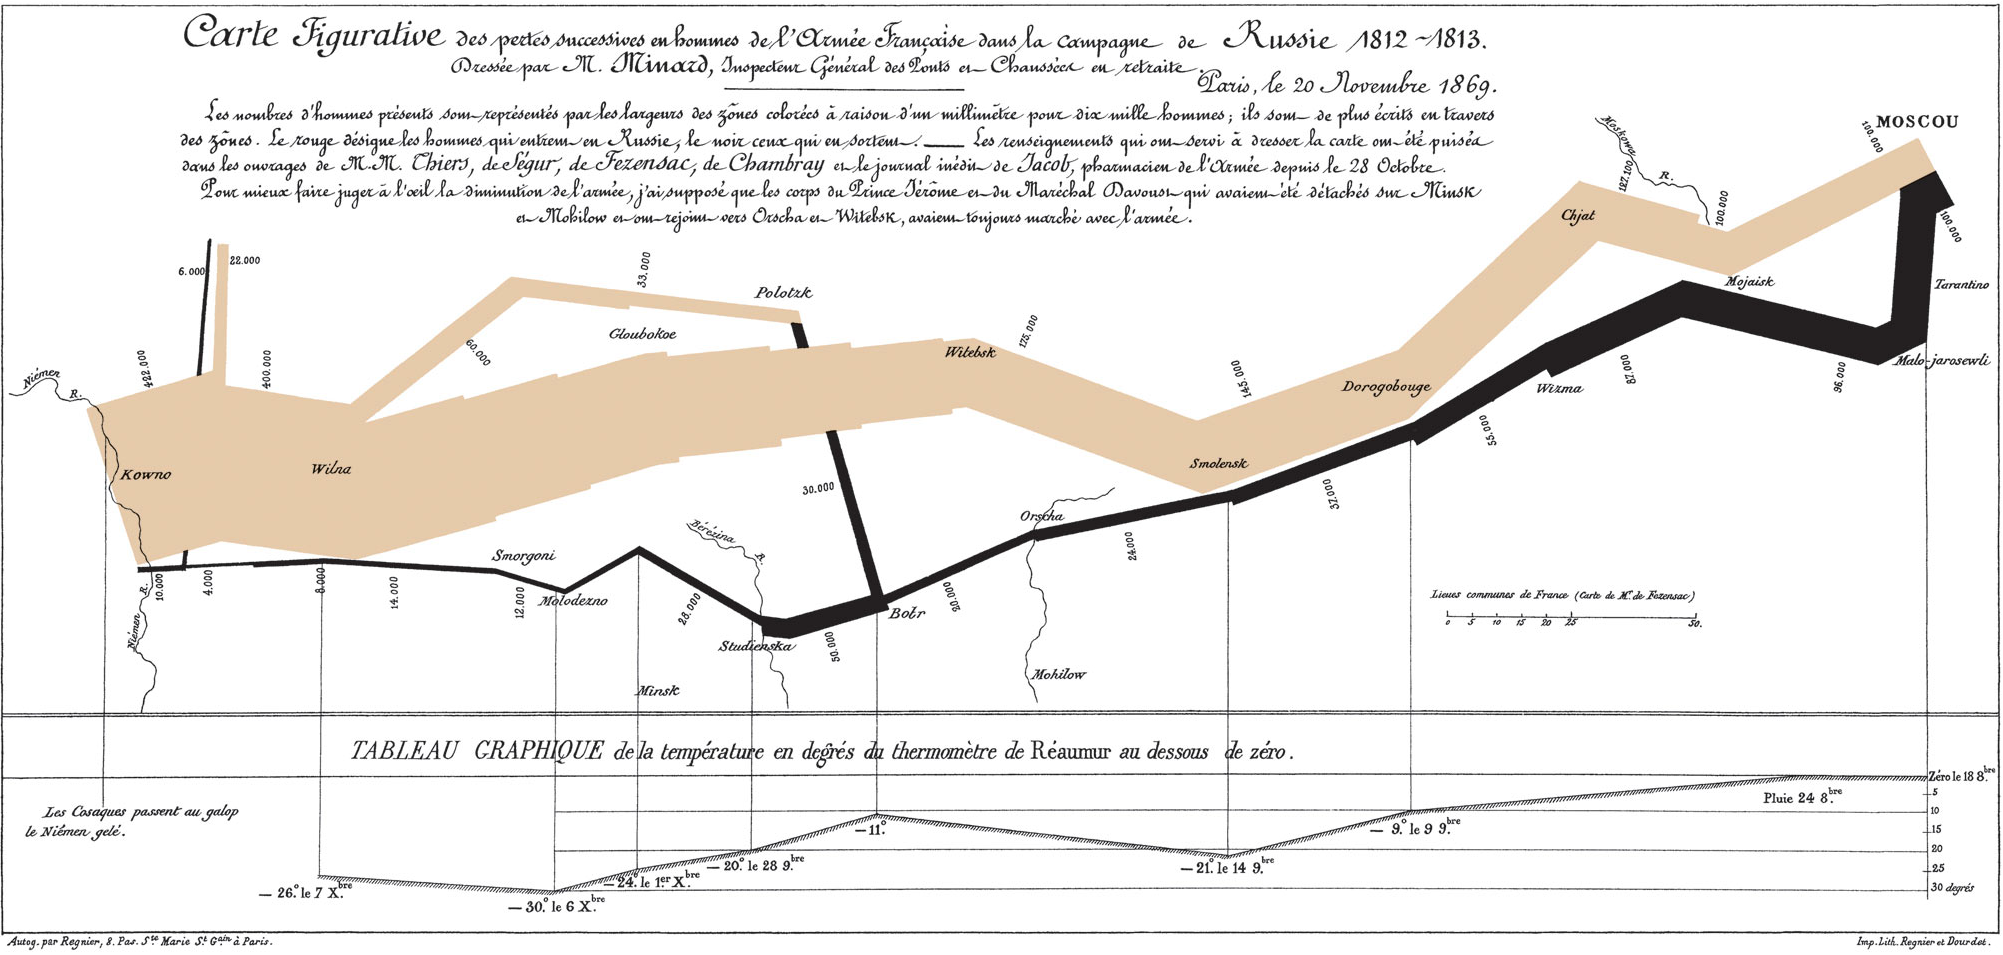
\includegraphics[width=27.82in]{images/Minard_timeline_map} \caption{Minards visualization of Napoleon's disasterous march to Moscow}\label{fig:minard}
\end{figure}

\section*{Why read this book}\label{why-read-this-book}


The aim of this book is help people make more graphs like Figure
\ref{fig:minard}). It links principles of graph design to examples that
are implemented in R, particularly the popular graphic package ggplot2.
The book provides a catalog of graphs and their design rationale
organized around general questions that graphs are typically used to
answer.

\section*{Structure of the book}\label{structure-of-the-book}


Chapter \ref{Introduction} introduces R and the tidyverse functions and
provides links for learning more about the basic capabilties of R.
Chapters \ref{Association} - \ref{Connection} each describe different
types of graphs that answer questions regarding association,
distribution, comparison, proportion, fluctionation, and connection.
Chapter \ref{Tables} briefly considers graphical elements in tables and
Chapters \ref{Polishing} - \ref{Interaction} discuss interactive graphs
and adjustments neeed for publication.

\section*{Software information and
conventions}\label{software-information-and-conventions}


I used the \textbf{knitr}\index{knitr} package \citep{xie2015} and the
\textbf{bookdown}\index{bookdown} package \citep{R-bookdown} to compile
the book. Most graphs have been created with \textbf{ggplot2}
{[}@\{Wickham2016a{]} and data manipulation is done with \emph{dplyr}.

\section*{Acknowledgments}\label{acknowledgments}


\BeginKnitrBlock{flushright}
\EndKnitrBlock{flushright}

\chapter*{About the Author}\label{about-the-author}


John D. Lee is a professor in the Department of Industrial and Systems
Engineering at the University of Wisconsin-Madison. He has~investigated
the issues of human-automation interaction, particularly trust
inautomation, for over 20 years. More specifically, his research
considers trust and acceptance, as well as issues of distraction and
engagement. He helped to edit the Handbook of Cognitive Engineering,
which focusses on human interaction with increasingly autonomous
systems. He is also a co-author of a popular textbook: Designing for
People: An introduction to human factors engineering
(\url{http://designing4people.com}).

\cleardoublepage 

\chapter{Introduction: Purposes, questions, and
audiences}\label{Introduction}

Information technology has brought large volumes of data that the
promise of deeper understanding the challenges most central to our
individual and collective existance.

Often this promise is not kept and data overwhelms rather than informs.

Well-crafted visualization can make data meaningful.

This book provides principles and examples for data visualization

Provides ways of addressing common challenges: remove legend (Section
\ref{AddingRemovingLabels}) reorder categories of a bar chart or facets
Creating Tufte inspired styles (Section \ref{tufte-slopegraph})

\section{Seeing meaning rather than
numbers}\label{seeing-meaning-rather-than-numbers}

Figure \ref{fig:blood-tab} shows a typical report of a medical
diagnostic test. The numerical summary shows the patient's values and
the range of standard values. The information is there to show if a
patient is dangerously outside the range, but a quick glance at the
table might miss these indications. Even a careful reading of the table
might miss warning signs, particularly if the critical information is in
the trend that requires looking at a second table on another tab. Figure
\ref{fig:blood-vis} shows the data relative to the high and low normal
range and makes deviations much more apparent. The ghosted points show
past results and roughly indicate trends.

\begin{figure}
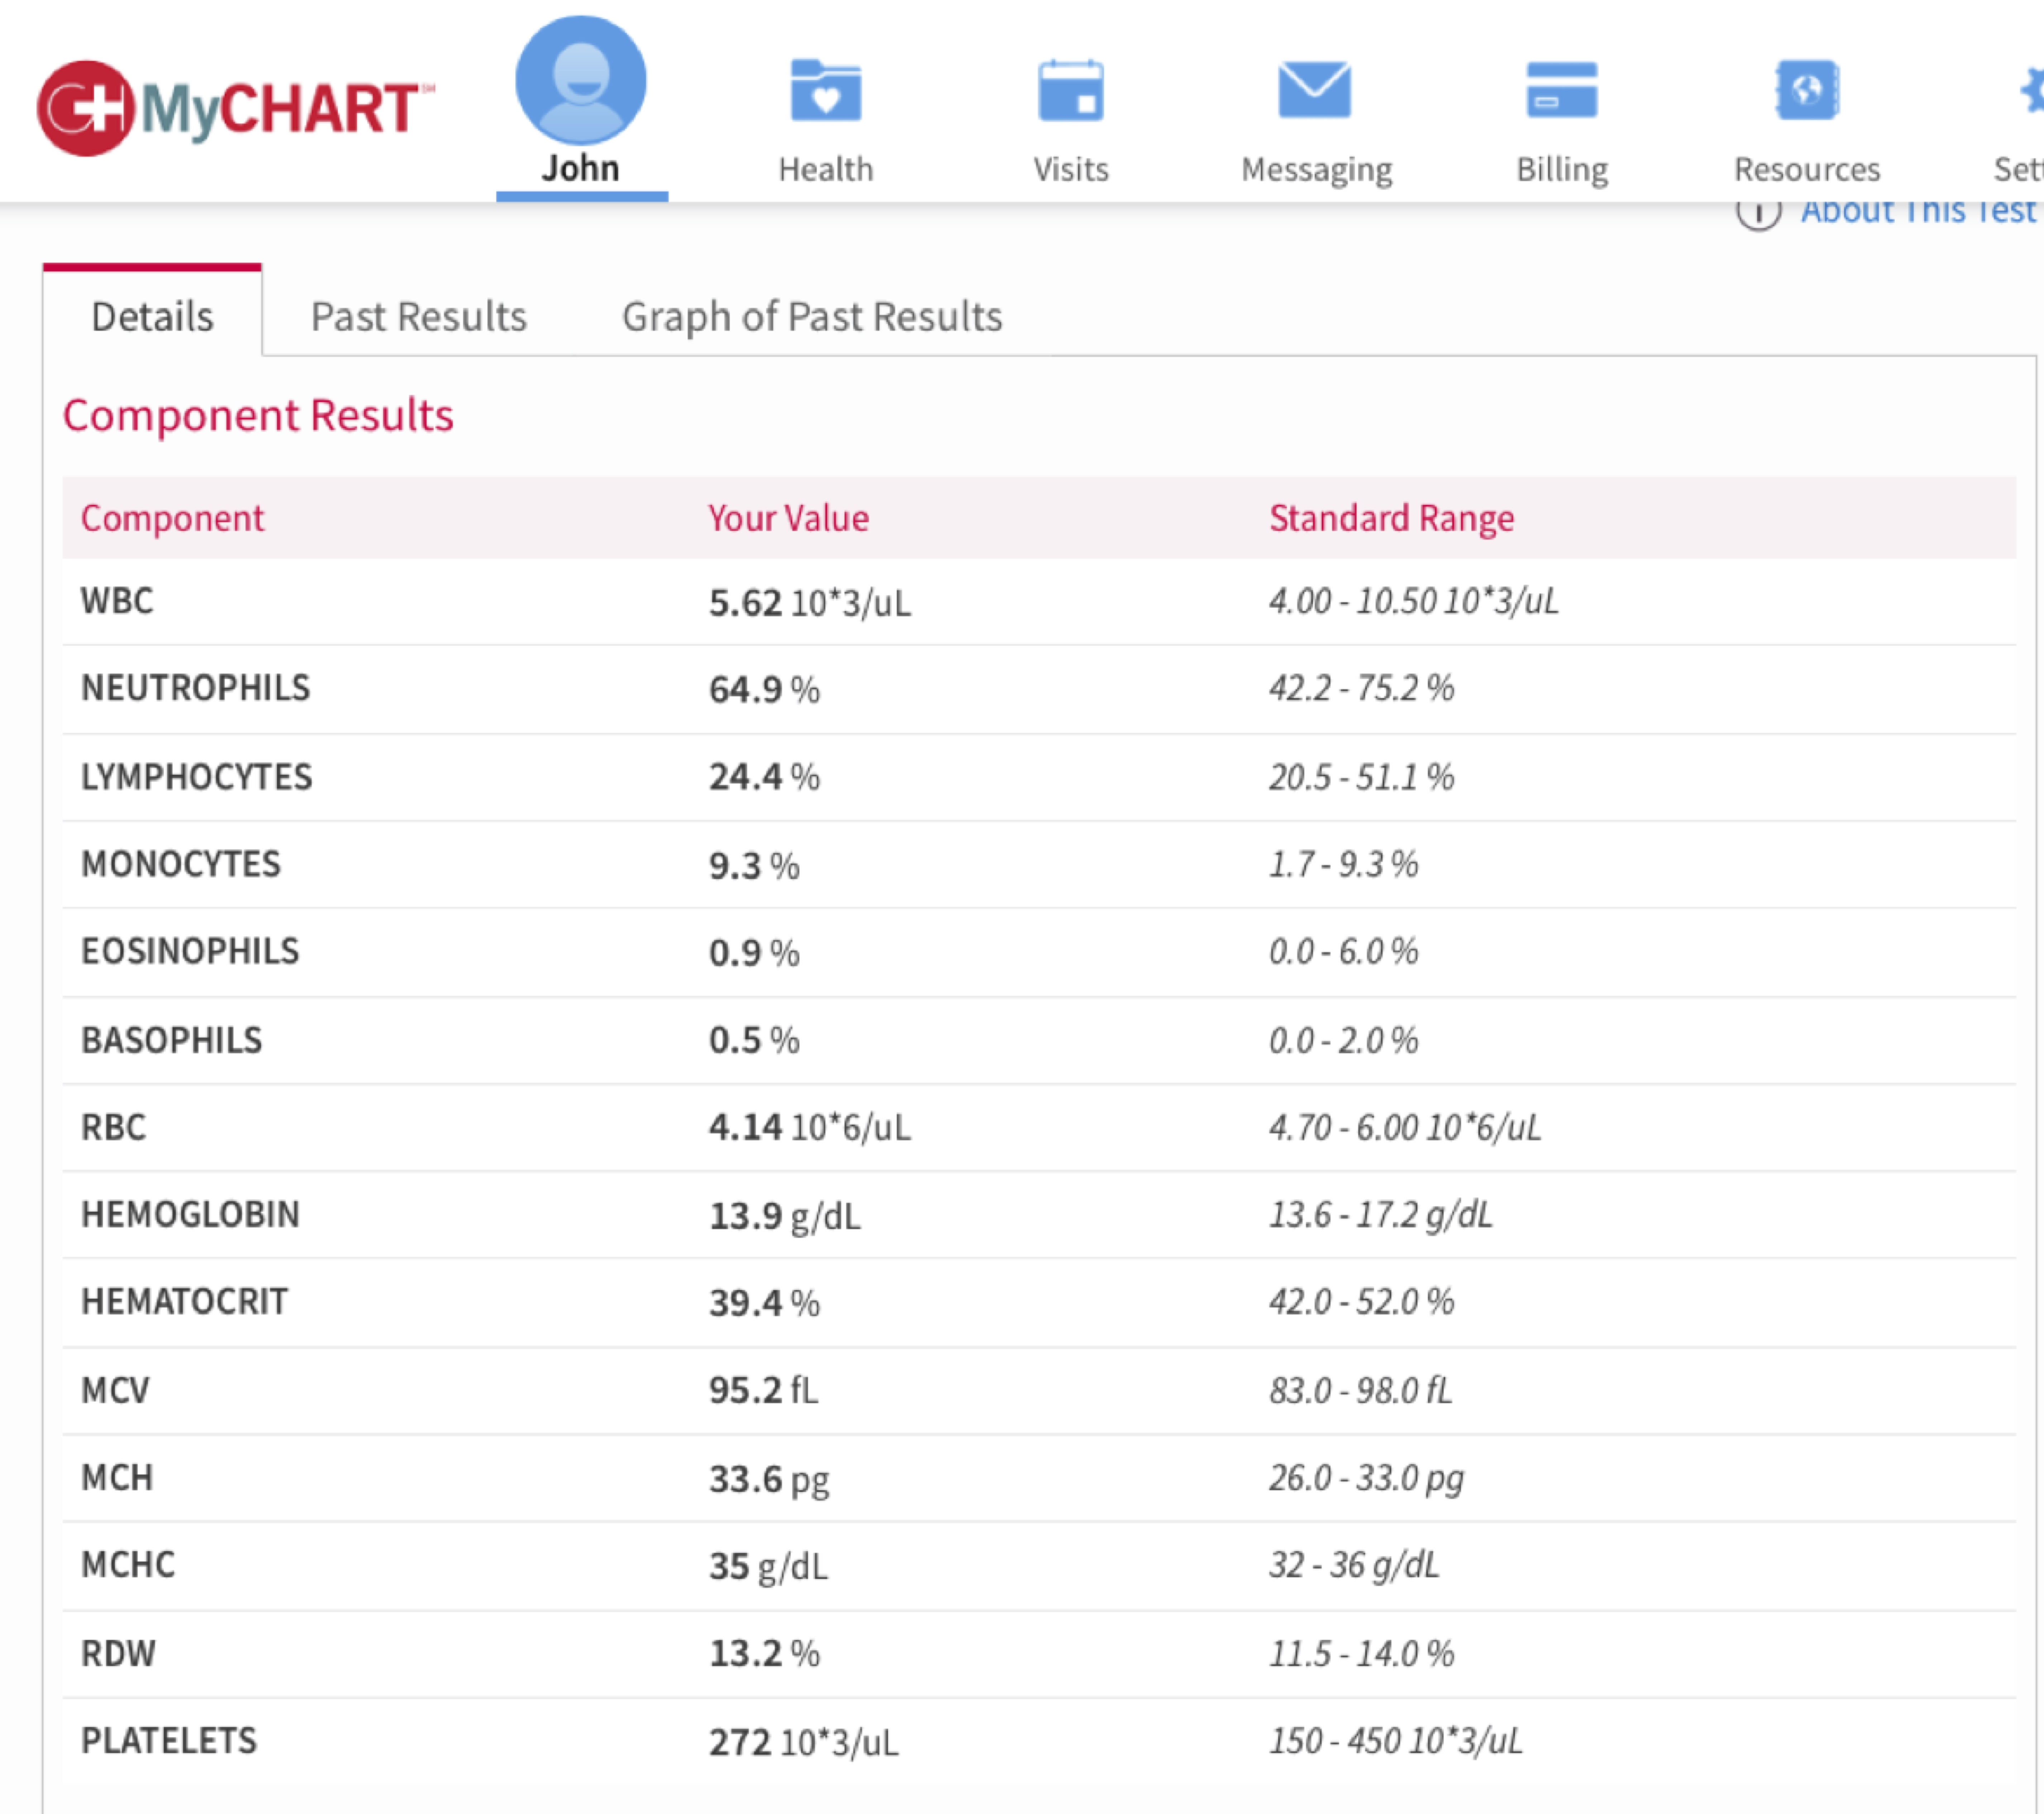
\includegraphics[width=79.25in]{images/Blood_table} \caption{A typical report of a medical test makes finding deviations from the normal range difficult.}\label{fig:blood-tab}
\end{figure}

\begin{verbatim}
## Warning: package 'bindrcpp' was built under R version
## 3.4.4
\end{verbatim}

\begin{figure}
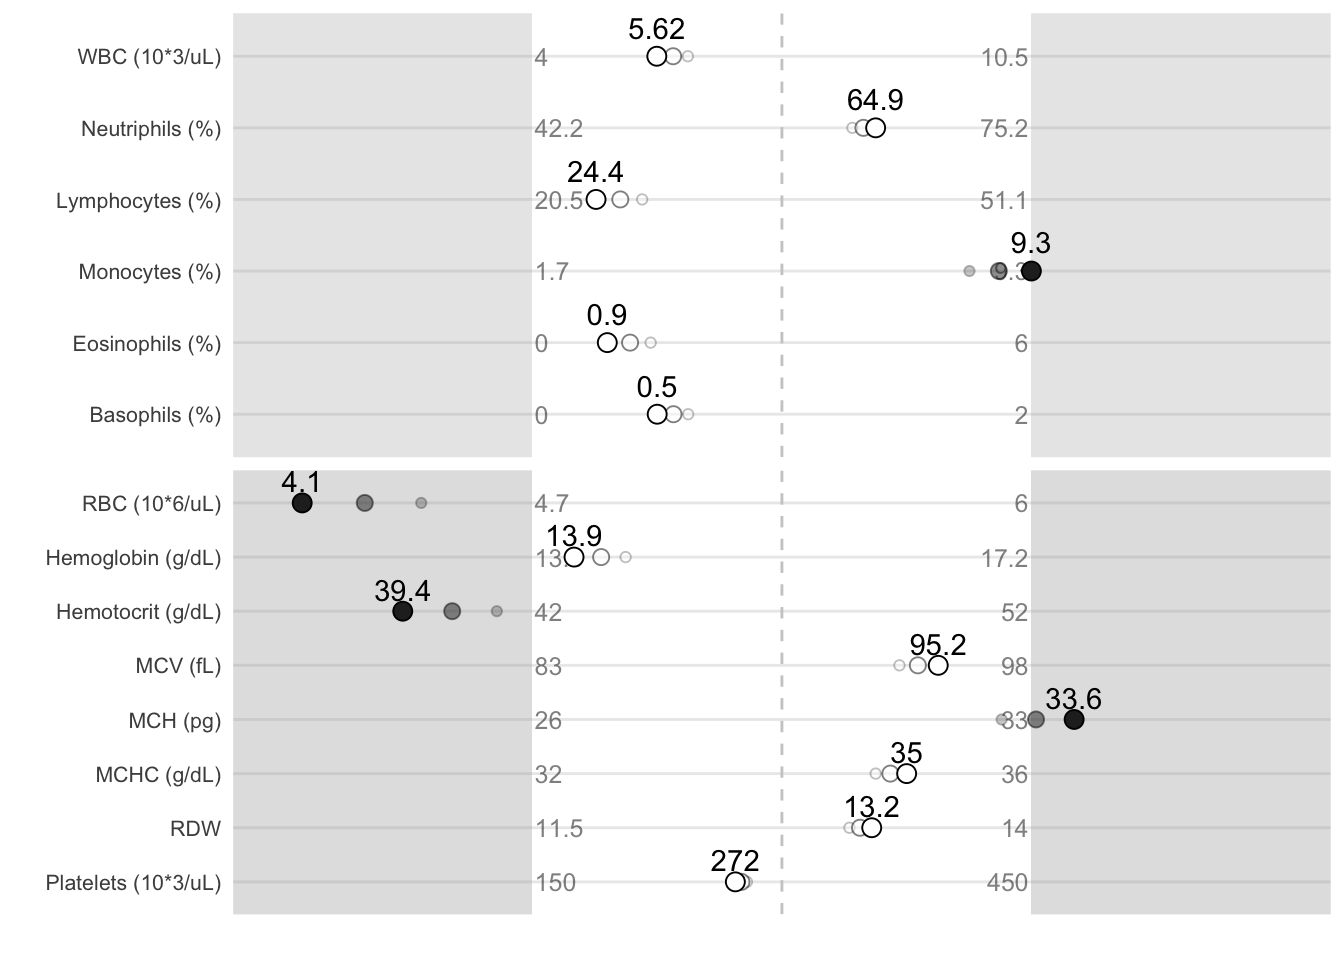
\includegraphics{visualizationwithggplot_files/figure-latex/blood-vis-1} \caption{A visualization of the same results makes the deviations pop out.}\label{fig:blood-vis}
\end{figure}

\section{Seeing more than summary
statistics}\label{seeing-more-than-summary-statistics}

The easy availability of sophisticated machine learning and statistical
models makes algorithmic interpretation of data tempting. However, such
interpretations can mislead, with similar outcomes produced by very
different underlying data.

Figure \ref{fig:anscombe-vis} shows four distinct sets of data. The
differences are obvious when graphed. One might expect that the typical
summary statistics--mean, standard deviation, and correlation--would
show equally stark differences. Table \ref{tab:anscombe-tab} shows this
is not the case. Each data set has the same summary statistics.

\begin{figure}
\centering
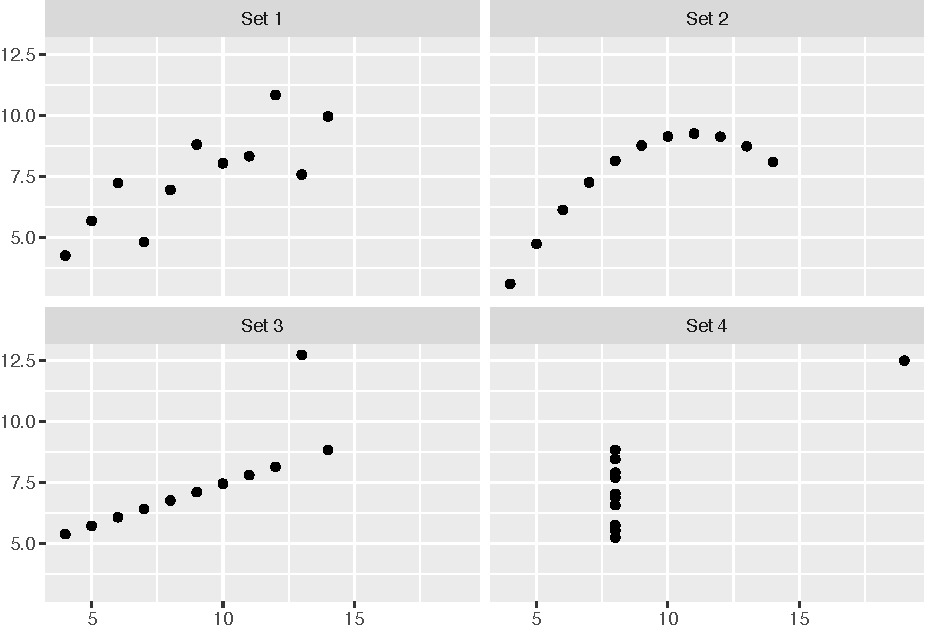
\includegraphics{visualizationwithggplot_files/figure-latex/anscombe-vis-1.pdf}
\caption{\label{fig:anscombe-vis}The Anscombe quartet and the limits of
summary statistics.}
\end{figure}

\begin{table}[t]

\caption{\label{tab:anscombe-tab}Four seemingly identical datasets that illustrate the limits of algorithmic interpretation.}
\centering
\begin{tabular}{lrrr}
\toprule
Data set & Mean & Standard deviation & Correlation\\
\midrule
Set 1 & 7.5 & 2.03 & 0.82\\
Set 2 & 7.5 & 2.03 & 0.82\\
Set 3 & 7.5 & 2.03 & 0.82\\
Set 4 & 7.5 & 2.03 & 0.82\\
\bottomrule
\end{tabular}
\end{table}

\section{Purpose and audience of
visualizations}\label{purpose-and-audience-of-visualizations}

Explore, inform, and engage \citep{Gelman2013}

Target audience: yourself, peers, scientists and engineers, public
(NYTimes ref)

Explore: the answer is unknown and audience is likely yourself and peers
involved in the research

Inform: the answer is known and the audience is likely a broader
audience of scientists, engineers, or manager not direclty involved in
the research.

Engage: the answer is known and must be communicated in an entertaining
way to those who may might neet to be drawn into readin the graph and
may not be familiar with conventions of scientific visualization, such
as box plots.

\section{What question to answer?}\label{what-question-to-answer}

\section{Storytelling with graphics}\label{storytelling-with-graphics}

\begin{itemize}
\tightlist
\item
  High-level principles for communication, such as ``Show don't tell''
\item
  Role of annotation in going beyond the data: direct attention and
  explain, as in Table \ref{tab:test}.
\end{itemize}

Based on
\url{https://www.rdocumentation.org/packages/HistData/versions/0.8-4/topics/Minard}

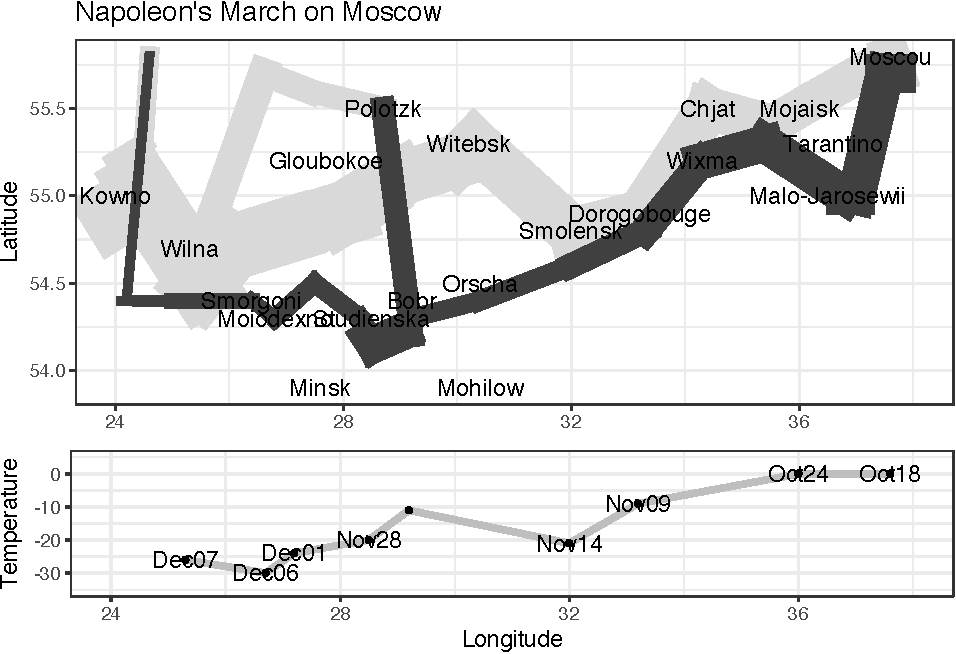
\includegraphics{visualizationwithggplot_files/figure-latex/unnamed-chunk-3-1.pdf}

\section{Data}\label{data}

This book is not about data reduction and data wrangling. The tidyverse
provides an intrgrated set of tools for data wrangling
\url{http://r4ds.had.co.nz}. This book uses data from the following
sources:

\url{https://www.kaggle.com}

\url{https://www.data.gov} Consumer complaint database, NTSB accident
database

\url{https://flowingdata.com/category/projects/data-underload/}

\url{http://www.wolframalpha.com}

R packages: HistData, babynames

Yao about data and web scraping and the package

\begin{Shaded}
\begin{Highlighting}[]
\NormalTok{## Read data from website}
\CommentTok{# sports <- read_tsv("https://github.com/halhen/viz-pub/raw/master/sports-time-of-day/activity.tsv")}


\NormalTok{## Happiness}
\CommentTok{# }
\NormalTok{happiness.df =}\StringTok{ }\KeywordTok{read.csv}\NormalTok{(}\StringTok{"data/world-happiness-report/2017.csv"}\NormalTok{)}
\KeywordTok{ggplot}\NormalTok{(happiness.df, }\KeywordTok{aes}\NormalTok{(Freedom, Happiness.Score)) }\OperatorTok{+}\StringTok{ }\KeywordTok{geom_point}\NormalTok{()}
\end{Highlighting}
\end{Shaded}

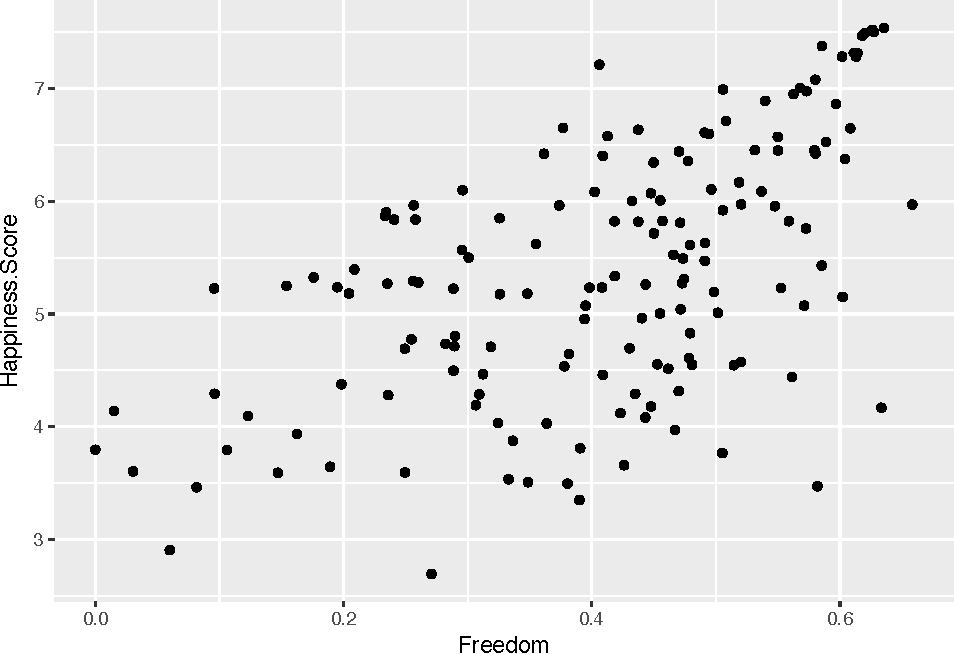
\includegraphics{visualizationwithggplot_files/figure-latex/happiness-plot-1.pdf}

\begin{Shaded}
\begin{Highlighting}[]
\NormalTok{## Chocolate}
\CommentTok{# chocolate.df = read.csv("flavors_of_cacao.csv")}
\CommentTok{# chocolate.df$Cocoa.Percent = as.numeric(chocolate.df$Cocoa.Percent)}
\CommentTok{# ggplot(chocolate.df, aes(Cocoa.Percent, Rating)) + geom_point()}


\NormalTok{## Police}
\NormalTok{## 2535 observations, Age, gender, how armed, state, threat, body cameraAll factors}
\NormalTok{ police.df =}\StringTok{ }\KeywordTok{read.csv}\NormalTok{(}\StringTok{"data/PoliceKillingsUS.csv"}\NormalTok{) }

\CommentTok{# Canadian vehicle specifications: http://www.carsp.ca/research/resources/safety-sources/canadian-vehicle-specifications/}
\end{Highlighting}
\end{Shaded}

\cleardoublepage 

\chapter{Visualization types and principles}\label{Principles}

\begin{verbatim}
## Warning: package 'igraph' was built under R version
## 3.4.4
\end{verbatim}

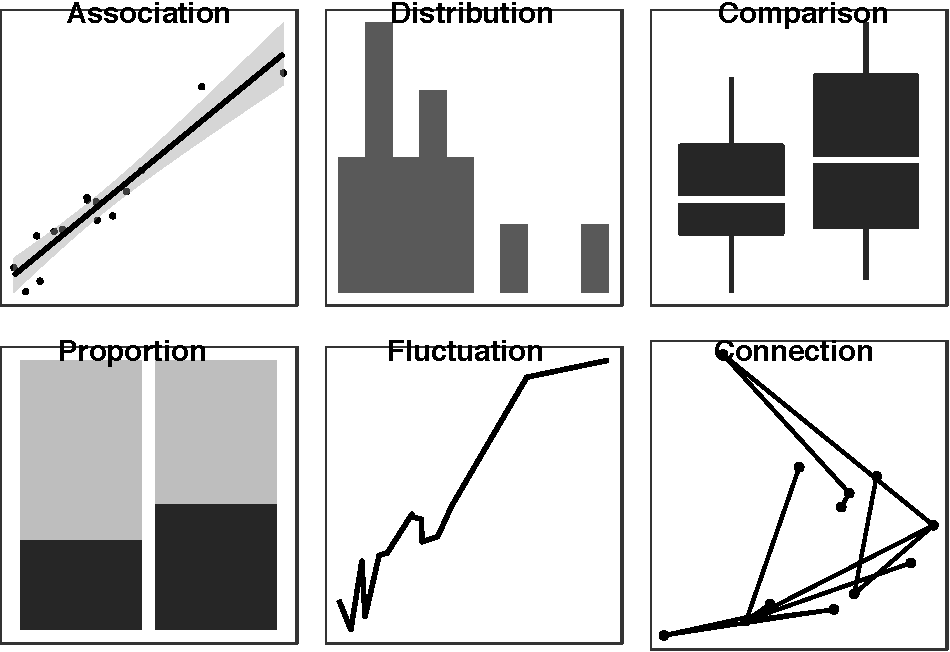
\includegraphics{visualizationwithggplot_files/figure-latex/graphtypes-1.pdf}

\section{Pairing questions and graph
types}\label{pairing-questions-and-graph-types}

Graphs answer questions about data by showing relationships and making
comparisons easier. Before creating a graph it is critical to specify
the questions and comparisons of interest. Figure \ref{fig:graphtypes}
shows common graphs and general questions they might answer. For
example, in the upper left is a graph that shows the association between
variables. This type of graph answers questions such as ``how does X
influence Y?'', as in ``does increasing the prices of gas reduce the
amount of driving?''. A scatter plot shows the strength and nature of
this association. Each graph in Figure \ref{fig:graphtypes} is suited to
a different question:

Graphs answer questions about data by showing relationships and making
comparisons easier. Before creating a graph it is critical to specify
the questions and comparisons of interest. Table \ref{tab:GraphTypes}
shows common graphs and general questions they might answer. For
example, in the upper left is a graph that shows the association between
variables. This type of graph answers questions such as how does X
influence Y, as in ``does increasing the prices of gas reduce the amount
of driving?''. A scatter plot shows the strength and nature of this
association.

\begin{itemize}
\tightlist
\item
  Association: What influences an outcome?
\item
  Distribution: What is the spread of the observations?
\item
  Comparision: How does one condition differ from another?
\item
  Proportion: What is the size of the components that make up the whole?
\item
  Fluctuation: How does the do observations vary over time?
\item
  Connection: How are the observations connnected over a map or network?
\end{itemize}

Combinations of questions, such as changes in distribution or proportion
over time

Questions in terms of patterns vs precision

Graph type and familiarity, pie charts Scatter plot to 2-density,
comparison to ranking, dotplot to violin or boxplot.

Graph types and volume of data.\\
More data requires abstraction. Some plots scale well others do not,
overplotting one example of scaling challenges with increasingly large
data.

More data points and more variables (e.g., time sequences, categories),
organize chapters to move from few points and few variables to many
(e.g., histogram to small multiple, to heatmap)

Types of data sets: Number of observations (independent, sequential)
Number variables (nominal, ordinal, interval)

\textasciitilde{}50 observations and 5 nominal and 7 interval variables
(mtcars, IIHS vehicle fatalities) \textasciitilde{}50 observations and 1
nominal and 4 interval variables (iris) \textasciitilde{}200
observations and 2 nominal and interval variables (10) (belts)
\textasciitilde{}50,000 observations an 10 nominal and interval
variables (diamonds)

The examples for each type of graphs represent one of many possible
representations. For example, the stacked bar chart addresses questions
of proportion, but so can pie charts and 3-D pie charts. How do you
choose between these alternatives? One consideration is to select
display dimensions that make it easy for people to make comparisons
needed to answer the questions---identify effective mapping between data
and display dimensions---which we turn to in the following section.

\section{Percpetual processes to be supported: Comparison, Detection,
Pattern
identification}\label{percpetual-processes-to-be-supported-comparison-detection-pattern-identification}

Attentional span Visual WM limits Preattentive cues Compatability
Conventions and familiarity

\subsection{Comparison}\label{comparison}

Differences between conditions, Compare to zero? Perceptual sensitivity
Proximity compatibility principle (enable relative rather than absolute
comparisons with reference lines and data ordering)

\subsection{Detection}\label{detection}

Outliers, deviations from assumptions Popout effects TODO Create figure
to show cost of conjunctive search and benefit of redundant coding

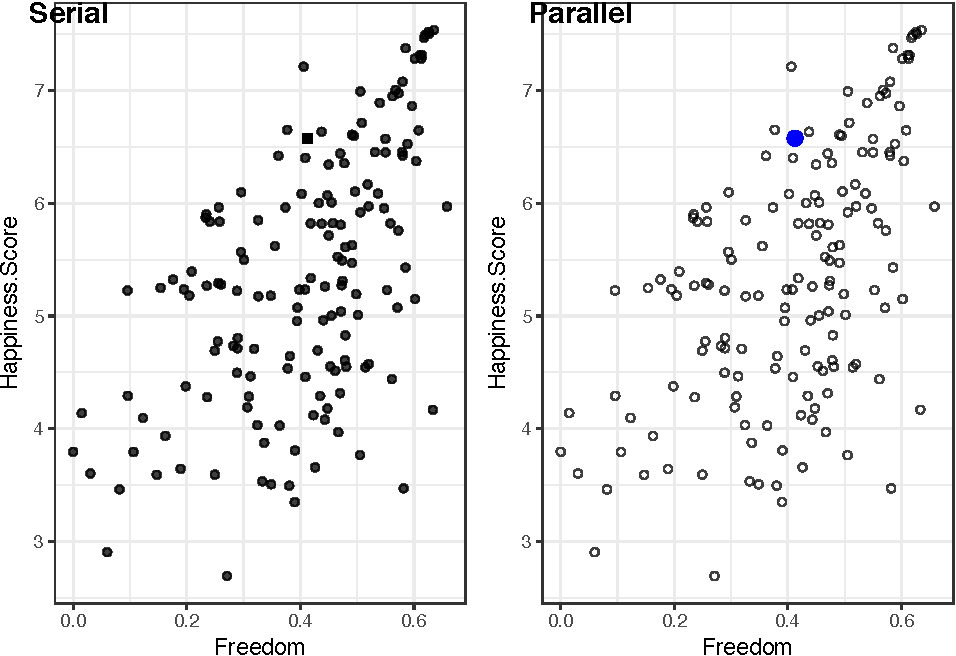
\includegraphics{visualizationwithggplot_files/figure-latex/scatterplot-popout-1.pdf}

\subsection{Pattern identification}\label{pattern-identification}

Associations, interactions, and changes over time Gestalt principles

Preattentive processing

TODO Create figure to show relative benefit of shape, intensity color
for grouping

Grouping and gestalt Similarity Continuity Connection Proximity
Enclosure Closure

TODO Figure ground showing data and summary vs summary and data

\section{Principles from general to
specific}\label{principles-from-general-to-specific}

\citep{Tufte1983}, \citep[\citet{Gelman2013a}]{Munzner2014}

\%ten guidelines \citep{Kelleher2011a}

\subsection{Identify audience, story, and key relationships
(Few)}\label{identify-audience-story-and-key-relationships-few}

\subsection{Focus attention and organize
reading}\label{focus-attention-and-organize-reading}

Group Prioritize Provide context Sequence

Be consistent, every difference should tell

\subsection{Annotate to show cause and explain
why}\label{annotate-to-show-cause-and-explain-why}

\subsection{Concrete details engage and are
memorable}\label{concrete-details-engage-and-are-memorable}

Connect to the world

\subsection{Enable comparisons and put data in
context}\label{enable-comparisons-and-put-data-in-context}

(Tufte) Scatter plot: Data points with linear and loess models Category
plot: Boxplot with individual data points Time series: Small multiples
with grand mean

Estimation errors and effort proportional to the absolute difference
from common baseline: reference lines provide a local baseline. TODO
Show tall bars with mean reference line

\subsection{Map types of variables to graph
features}\label{map-types-of-variables-to-graph-features}

Mapping data to graph features \citep{Cleveland1985}

For the purposes of display design, three different data types guide the
choice of display dimensions: interval, ordinal, and nominal
\citep{Cleveland1985}. Interval data include real or integer numbers
(e.g., height and weight), ordinal data are categories that have a
meaningful order (e.g., compact, mid-size, and full-size cars), and
nominal data are categories that have no order (e.g., male, female).
Each data type can be represented with one of several graph dimensions,
such as color or position, but certain mapping support more accurate
judgments.

Size of circle: map to radius or the area TODO create plot to show map
to radius and area

TODO show good and bad mappings

color \citep{Silva2011}

\begin{Shaded}
\begin{Highlighting}[]
\NormalTok{data =}\StringTok{ }\KeywordTok{read.csv}\NormalTok{(}\StringTok{'data/DataAestheticMapping.csv'}\NormalTok{)}

\NormalTok{data}\OperatorTok{$}\NormalTok{Type =}\StringTok{ }\KeywordTok{factor}\NormalTok{(data}\OperatorTok{$}\NormalTok{Type, }\DataTypeTok{levels=}\KeywordTok{c}\NormalTok{(}\StringTok{"Interval"}\NormalTok{, }\StringTok{"Ordinal"}\NormalTok{, }\StringTok{"Nominal"}\NormalTok{))}

\KeywordTok{ggplot}\NormalTok{(data, }\KeywordTok{aes}\NormalTok{(Type, }\KeywordTok{reorder}\NormalTok{(Rank, }\OperatorTok{-}\NormalTok{Rank), }\DataTypeTok{group =}\NormalTok{ Aesthetic)) }\OperatorTok{+}
\StringTok{  }\KeywordTok{geom_line}\NormalTok{(}\DataTypeTok{alpha =}\NormalTok{ .}\DecValTok{4}\NormalTok{, }\DataTypeTok{size =} \FloatTok{2.5}\NormalTok{) }\OperatorTok{+}
\StringTok{  }\KeywordTok{geom_text}\NormalTok{(}\KeywordTok{aes}\NormalTok{(}\DataTypeTok{label =}\NormalTok{ Aesthetic), }\DataTypeTok{size =} \DecValTok{5}\NormalTok{) }\OperatorTok{+}
\StringTok{  }\KeywordTok{ylab}\NormalTok{(}\StringTok{"Rank"}\NormalTok{) }\OperatorTok{+}\StringTok{ }\KeywordTok{xlab}\NormalTok{(}\StringTok{"Data type"}\NormalTok{) }\OperatorTok{+}
\StringTok{  }\KeywordTok{theme_bw}\NormalTok{()}
\end{Highlighting}
\end{Shaded}

\begin{figure}
\centering
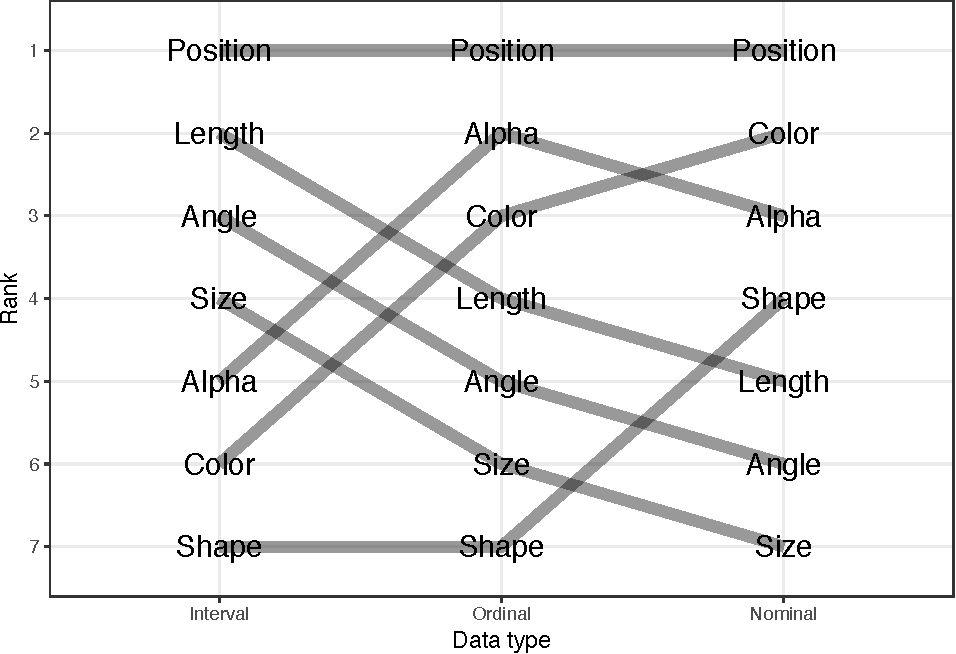
\includegraphics{visualizationwithggplot_files/figure-latex/perceptual-sensitivity-1.pdf}
\caption{\label{fig:perceptual-sensitivity}Aesthetic mapping.}
\end{figure}

\%TODO figure for mapping types of data and graph dimensions
\citep{Cleveland1985}

Figure XX shows seven ways to code these data \citep{Cleveland1985}. For
all three types of data, position, such as the horizontal or vertical
placement of a point in a graph, support the most precise judgments. The
other ways of coding information depend on the type of data: hue is a
poor choice for interval data, but a good choice for nominal data, as is
shape. Because shape and color have no natural mapping to magnitude,
they are a poor choice for interval and ordinal data. Magnitude is best
represented by position on a common scale, followed by position on an
unaligned scale, length and then angle, followed by size
\citep[\citet{Cleveland1985}]{Munzner2014}. Because size and angles are
relatively hard to judge, pie charts are not a good way to represent
proportions.

Limits of absolute judgment underlie the effectiveness of coding data
with various display dimensions. Coding nominal data with more than
seven hues will exceed people's ability and so they would not be able to
reliably link lines on a graph to categories. Data presented on aligned
scales, such as the bottom category in a stacked bar chart, can be
judged very precisely, but the limits of absolute judgment make
interpreting the upper categories more difficult. This means that the
bottom category of a stacked bar chart should be chosen carefully.
Generally, avoid placing data on unaligned scales. Instead, support
relative judgments based on a common scale. The circular format of pie
charts means that there are no aligned scales and is another reason why
they are not as effective as stacked bar charts.

Because visualization involves multiple conceptual dimensions, a natural
choice is to use three-dimensional Euclidian space. However,
three-dimensional figures make accurate comparisons difficult due the
ambiguity of rendering three dimensions on a two dimensional plane. Of
all the ways to represent a quantity, the volume of a three-dimensional
object leads to the most inaccurate judgments \citep{Munzner2014}.

Another important conceptual dimension is time. Time, like space, is
compatibly mapped to display dimension of position, often advancing from
left (past) to right (future). Time can also be directly mapped to
display time via animation. Animated graphs can be compelling, but they
require working memory to track objects across the display and so
severely limit the number of data points that can be compared.
Interactive visualization described in Chapter 10 can give control with
a slider and avoids this limit to some degree.

\subsection{Ensure proximity
compatibility}\label{ensure-proximity-compatibility}

Proximity compatibility and legend: link to line, orientate to match
orientation in graph, sequence to match sequence in graph

Visual attention must sometimes do a lot of work, traveling from place
to place on the graph, and this effort can hinder graph interpretation.
Hence, it is important to construct graphs so things that need to be
compared (or integrated) are either close together in space or can be
easily linked perceptually by a common visual code. This, of course, is
a feature for the proximity compatibility principle (A3) and can apply
to keeping legends close to the lines that they identify, rather than in
remote captions or boxes. Similarly, when the slopes and intercepts of
two lines need to be compared, keep them on the same panel of a graph
rather than on separate panels. The problems of low proximity will be
magnified as the graphs contain more information---more lines.
Similarly, in a box plot with many categories people will be able to
compare categories that are close to each other more precisely than
those that are separated. You should order categories so that those to
be compared are closest.

Proximity goes beyond physical distance. A line linking points on a
timeline can enhance proximity as can color and shape. Lines and color
can be effective ways of making groups of points in a network diagram
``closer'', and easier to interpret as a group. Objects with identical
colors tend to be associated together, even when they are spatially
separated. Furthermore a unique color tends to stand out. It is also the
case that space is compatibly mapped to space, so that visualization of
geographic areas is best accomplished when the dimensions of rendered
space correspond to the dimensions of displayed space--a map.

As with its application to other display designs, the proximity
compatibility principle means that the visual proximity of elements of
the graph need to correspond to the mental proximity needed to interpret
this information. For graphs, this means the questions and comparisons
the graph is intended to address should specify what is ``close'' in the
graph.

\subsection{Legibility and
consistency}\label{legibility-and-consistency}

As with other types of displays, issues of legibility are again
relevant. However, in addition to making lines and labels large enough
to be readable, a second critical point relates to discriminability
(P9). Too often, lines that have very different meanings are
distinguished only by points that are highly confusable, as in the graph
on the left of Figure XX. Here incorporating redundant coding of
differences can be quite helpful. In modern graphics packages, color is
often used to discriminate lines, but it is essential to use color
coding redundantly with another salient cue. Why? As we noted in Chapter
4, not all viewers have good color vision, and a non-redundant colored
graph printed from a black and white printer or photocopied may be
useless.

\subsection{Maximize data/ink ratio}\label{maximize-dataink-ratio}

(Tufte) * Maximize data to create rich representation, minimize
extraneous non-data elements

\begin{itemize}
\tightlist
\item
  Minimize non-data elements: bar charts rather than 3-D pie
\end{itemize}

Annotate to integrate interpretation and data

Simplify to amplify content

Simplify content to amplify point

\subsection{Manage clutter with grouping and
layering}\label{manage-clutter-with-grouping-and-layering}

\begin{itemize}
\tightlist
\item
  Match data type to appropriate aesthetics (Cleveland) Only position
  good for all data types: Focus on 2d-plane and relative judgments
  Consider data type: size better than color for interval data
\end{itemize}

Graphs can easily become cluttered by presenting more lines and marks
than the actual information they convey. As we know, clutter can be
counterproductive , and this has led some to argue that the data-ink
ratio should always be maximized \citep{Tufte1983}; that is, the
greatest amount of data should be presented with the smallest amount of
ink. While adhering to this guideline is a valuable safeguard against
the excessive ink of ``chart junk'' graphs, such as those that
unnecessarily put a 2-D graph into 3-D perspective, the guideline of
minimizing ink can however be counterproductive if carried too far.
Thus, for example, the ``minimalist'' graph in center of Figure X, which
maximizes data-ink ratio, gains little by its decluttering and loses a
lot in its representation of the trend, compared to the line graph on
the right Figure XX. The line graph contains an emergent
feature---slope---which is not visible in the dot graph. The latter is
also much more vulnerable to the conditions of poor viewing (or the
misinterpretation caused by the dead bug on the page!).

\%Figure 21. Space shuttle launches, temperature and O-ring damage.
\%TODO I love the example, but A more elaborated caption is needed to
direct reader's attention to the problem.

In some cases, the poor data to ink ratio and prevalence of chart junk
might create engaging graphics, other times it can be annoying, but in
presenting engineering data it can undermine the quality of life and
death decisions. Figure 20 shows the graphic used to support the launch
decision associated with the disastrous flight of the Space Shuttle
Challenger the data presented in this way makes it difficult to assess
the effect of temperature on O-ring damage, which may have encouraged
the managers to launch in cold weather \citep{Tufte1997}.

Figure X shows that you can increase the data-to-ink ratio by reducing
the ``ink'' devoted to non-data elements. Another way to increase the
data-to-ink ratio is to include more data. More data can take the form
of reference lines and multiple small graphs, as in Figure XX. More data
can also take the form of directly plotting the raw data rather than
summary data.

Figure \ref{fig:trip-dur} shows an extreme version, in which each data
point represents one of approximately 693,000 trips reported in the 2009
travel survey XXcite FHWA2011. The horizontal axis indicates the
duration and the vertical axis shows distance of each trip. The diagonal
lines of constant speed place these data in context by showing very slow
trips---those under the 3mph line---and very fast trips---those over the
90mph line. Histograms at the top and side show the distribution of trip
duration and distance. The faint vertical and horizontal lines show the
mean duration and distance. Like other visualizations that include the
raw data, this visualization shows what is behind the summary
statistics, such as mean trip distance and duration.

Showing the underlying data has the benefit of providing a more complete
representation, but it can also overwhelm people. Data can create
clutter. One way to minimize clutter is by grouping and layering the
data. In the case of Figure \ref{fig:trip-dur} this means making the
individual data points small and faint.

\begin{figure}
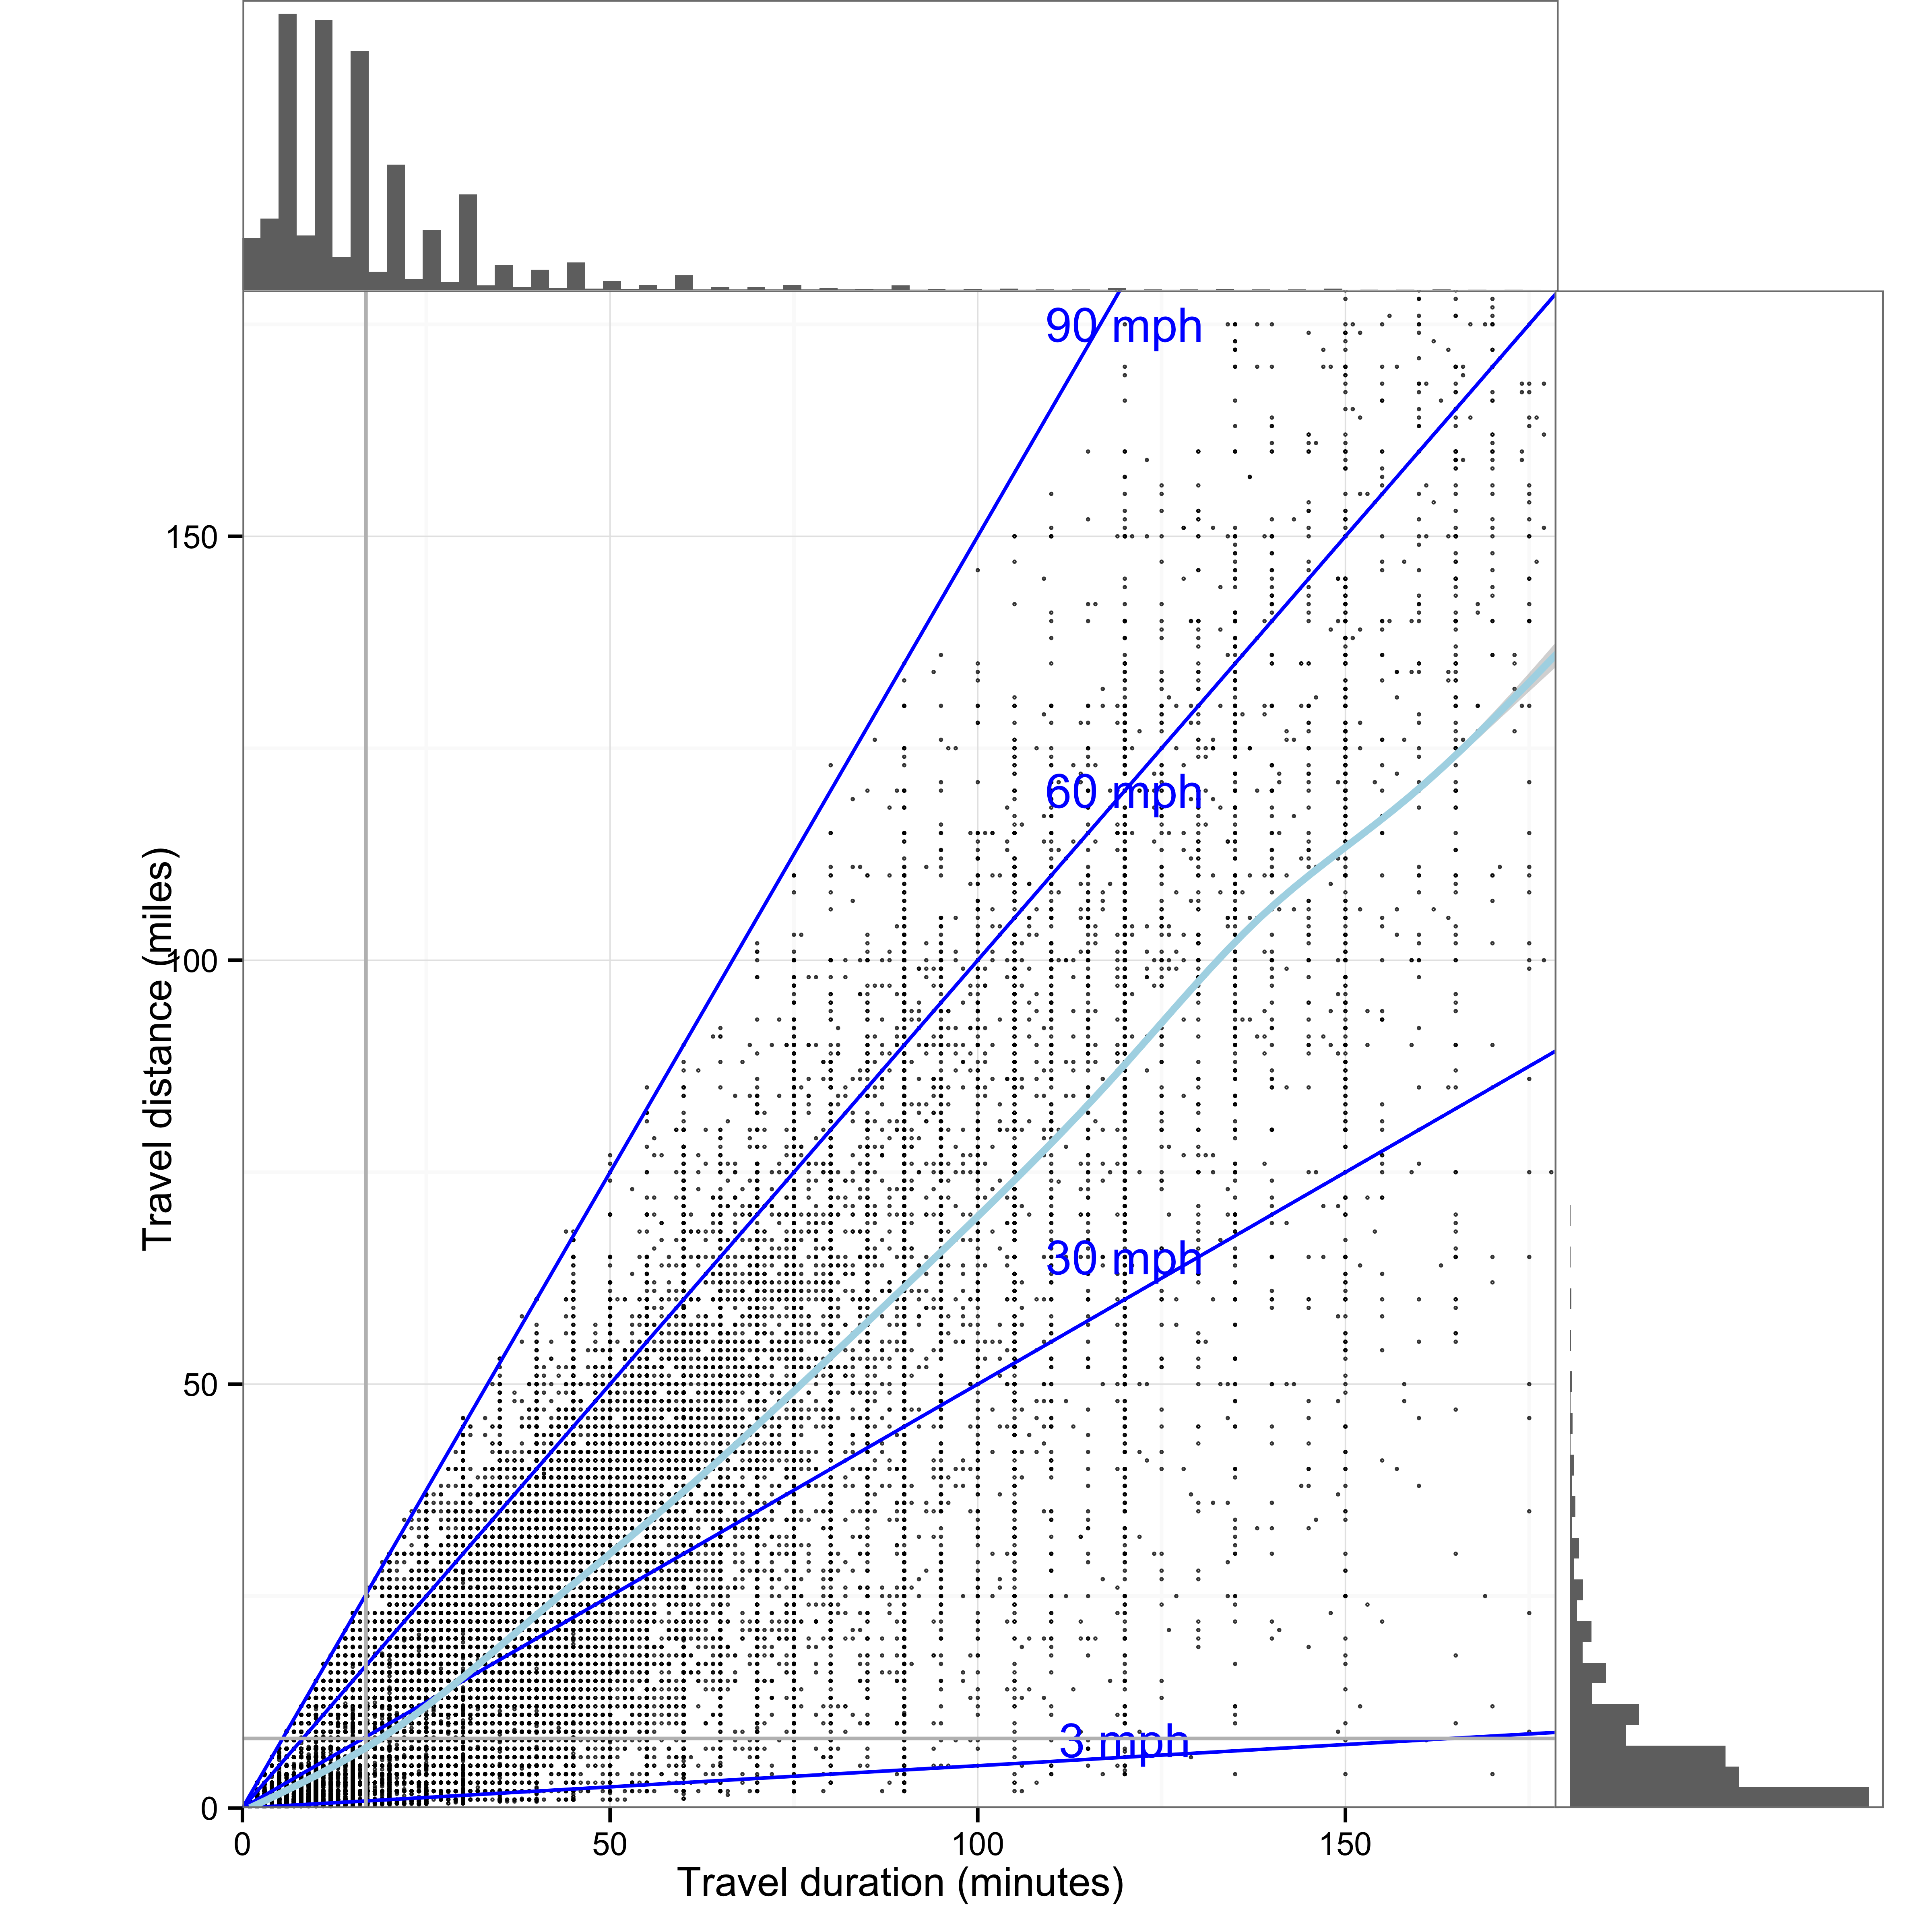
\includegraphics[width=66.67in]{images/Trip_Dist_Dur} \caption{An example of extreme data-to-ink with over 693,000 data points}\label{fig:trip-dur}
\end{figure}

\section{Overview of examples}\label{overview-of-examples}

Simple, few variables, few observations and single graphical element to
and complex, many observations to combitions of graphical elements

\cleardoublepage 

\chapter{Association--scatterplots}\label{Association}

\section{Basic elements of the grammar of
graphics}\label{basic-elements-of-the-grammar-of-graphics}

\begin{longtable}[]{@{}ll@{}}
\caption{\label{tab:test} Summary of ggplot element.}\tabularnewline
\toprule
ggplot element & Description\tabularnewline
\midrule
\endfirsthead
\toprule
ggplot element & Description\tabularnewline
\midrule
\endhead
Data & ggplot uses a dataframe as input (e.g., data =
mtcars.data)\tabularnewline
Geoms & geometric element (e.g., geom\_point, geom\_bar)\tabularnewline
Mapping & links data variables to aesthetic dimensions (aes) (e.g.,
aes(x = cyl, y = mpg))\tabularnewline
Setting & specifies value of aesthetic dimension directly (e.g., colour
= ``blue'')\tabularnewline
Layers & add components to base plot, most often geoms (additional
layers added with ``+'')\tabularnewline
Stats & statistical summary, such as density or count; each geom has a
default statistic\tabularnewline
Position & adjusts the location of the plotted geom\tabularnewline
Annotations & text and graphical overlays\tabularnewline
Coordinate system & Cartesian, polar or small multiple
facets\tabularnewline
Themes & sets of plot parameters (e.g., font, background)\tabularnewline
\bottomrule
\end{longtable}

\section{Simple scatterplot}\label{simple-scatterplot}

The simplest plot must include data, aesthetic mapping, and geom a
geometric element. The data must be organized with each observation as a
row and each variable as a column. For a scatterplot the geometric
element is a point, and the aesthetic mapping links variables to
properties of the geometric element. For a scatterplot this would be the
x and y position of the point. the the point the x and y position must
be specified, but other properties, such as color, size, alpha level,
and shape, can be mapped to variables. These properties of the geometric
element can also be set to specific values, such as specifying the color
of the point.

Figure \ref{fig:simple-scatterplot} shows the ggplot2 code and
associated scatterplot. The equation used to specify the plot implicitly
specifies the values by their position, such as data being identifed as
following ``ggplot(''. The following speciifcations are equivalent:

`` ggplot(data = mtcars.df, mapping = aes(x = wt, y = mpg)) +
geom\_point(colour = ``darkblue'')

ggplot(mtcars.df, aes(wt, mpg)) + geom\_point(colour = ``darkblue'') ``

\begin{Shaded}
\begin{Highlighting}[]
\KeywordTok{library}\NormalTok{(tidyverse)}

\NormalTok{mtcars.df =}\StringTok{ }\NormalTok{mtcars}

\KeywordTok{ggplot}\NormalTok{(}\DataTypeTok{data =}\NormalTok{ mtcars.df, }\DataTypeTok{mapping =} \KeywordTok{aes}\NormalTok{(}\DataTypeTok{x =}\NormalTok{ wt, }\DataTypeTok{y =}\NormalTok{ mpg)) }\OperatorTok{+}
\StringTok{  }\KeywordTok{geom_point}\NormalTok{(}\DataTypeTok{colour =} \StringTok{"darkblue"}\NormalTok{)}
\end{Highlighting}
\end{Shaded}

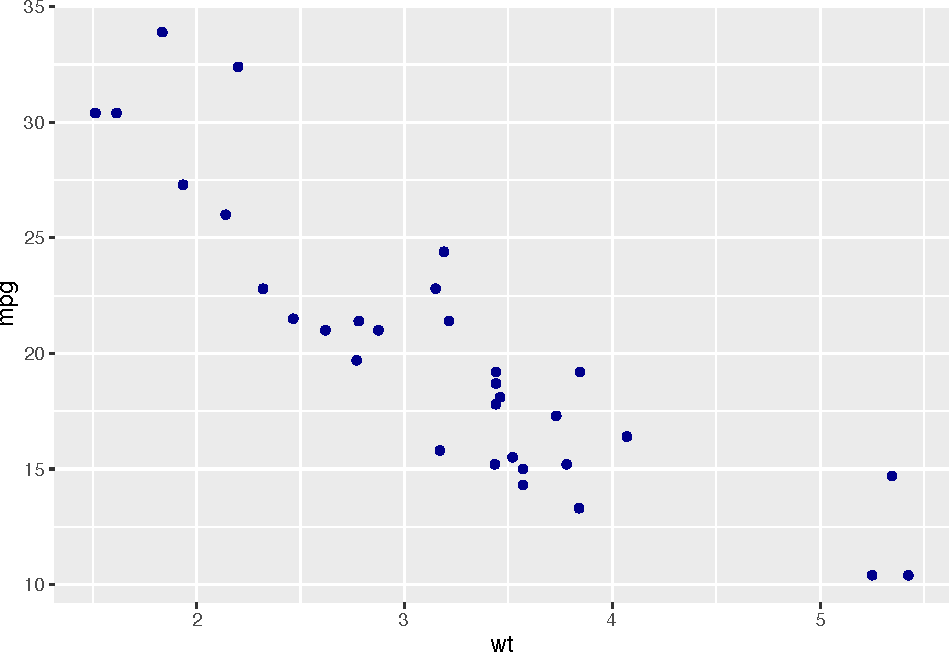
\includegraphics{visualizationwithggplot_files/figure-latex/simple-scatterplot-1.pdf}

A powerful feature of ggplot2 is the abilty to add layers of geometric
elements to a plot. Each layer can have its own data, mapping of
aesthetic properties, and setting of aesthetic properties. The data and
mapping specified in the base plot statement--``ggplot(data = mtcars.df,
mapping = aes(x = wt, y = mpg))''--are global and apply to all layers,
but can overridden by the any mappings specific to a layer. Figure
\ref{fig:scatterplot-layering} shows a layer of red circles based on a
subset of the data.

\begin{Shaded}
\begin{Highlighting}[]
\NormalTok{fourcyl.mtcars.df =}\StringTok{ }\NormalTok{mtcars.df }\OperatorTok\StringTok{ }\KeywordTok{filter}\NormalTok{(cyl}\OperatorTok{==}\DecValTok{4}\NormalTok{)}

\KeywordTok{ggplot}\NormalTok{(}\DataTypeTok{data =}\NormalTok{ mtcars.df, }\DataTypeTok{mapping =} \KeywordTok{aes}\NormalTok{(}\DataTypeTok{x =}\NormalTok{ wt, }\DataTypeTok{y =}\NormalTok{ mpg)) }\OperatorTok{+}
\StringTok{  }\KeywordTok{geom_point}\NormalTok{(}\DataTypeTok{colour =} \StringTok{"darkblue"}\NormalTok{) }\OperatorTok{+}\StringTok{ }
\StringTok{  }\KeywordTok{geom_point}\NormalTok{(}\DataTypeTok{data =}\NormalTok{ fourcyl.mtcars.df, }\DataTypeTok{colour =} \StringTok{"red"}\NormalTok{, }\DataTypeTok{shape =} \DecValTok{21}\NormalTok{, }\DataTypeTok{size =} \DecValTok{4}\NormalTok{)}
\end{Highlighting}
\end{Shaded}

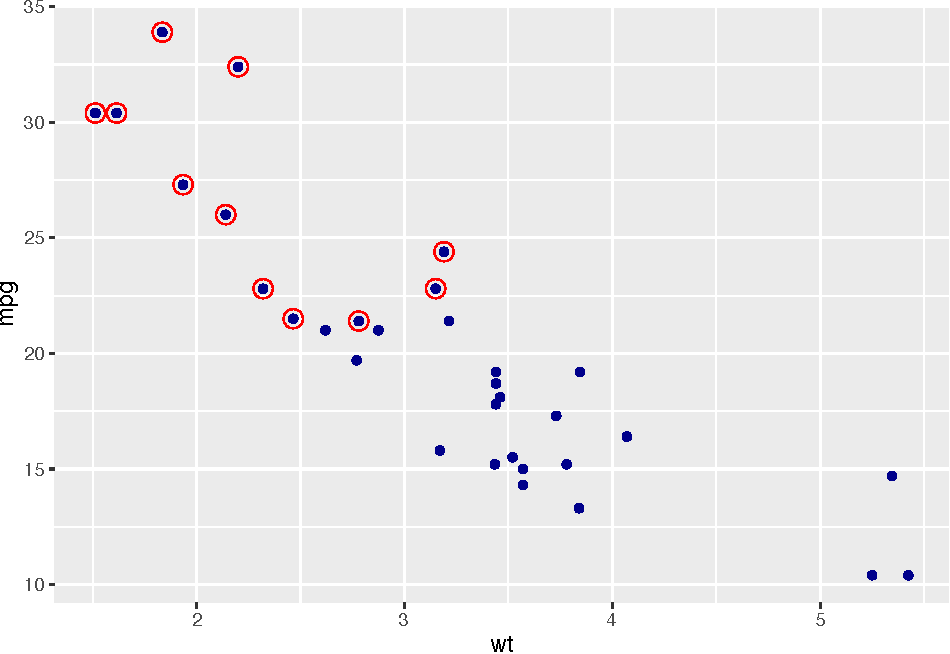
\includegraphics{visualizationwithggplot_files/figure-latex/scatterplot-layering-1.pdf}

\section{Scatterplot with additional
mappings}\label{scatterplot-with-additional-mappings}

The scatterplot typically maps variables to the x and y position of the
points, but ggplot allows for other mappings. Figure
\ref{fig:scatterplot-mapping} shows mapping variables to the fill and
size of the points. The shape, stroke, and color of the points are set
to values they could also be mapped, which could quickly overload the
graph. Note that only shapes 21-25 in Figure \ref{fig:symbols} can
include fill and stroke, with the other symbols color determines the
color of the whole symbol not just the border.

\begin{Shaded}
\begin{Highlighting}[]
\KeywordTok{ggplot}\NormalTok{(}\DataTypeTok{data =}\NormalTok{ mtcars, }\DataTypeTok{mapping =} \KeywordTok{aes}\NormalTok{(}\DataTypeTok{x =}\NormalTok{ wt, }\DataTypeTok{y =}\NormalTok{ mpg, }\DataTypeTok{fill =}\NormalTok{ hp, }\DataTypeTok{size =} \DecValTok{1}\OperatorTok{/}\NormalTok{qsec)) }\OperatorTok{+}\StringTok{ }
\StringTok{  }\KeywordTok{geom_point}\NormalTok{(}\DataTypeTok{shape =} \DecValTok{21}\NormalTok{, }\DataTypeTok{colour =} \StringTok{"darkred"}\NormalTok{, }\DataTypeTok{stroke =} \DecValTok{2}\NormalTok{.) }
\end{Highlighting}
\end{Shaded}

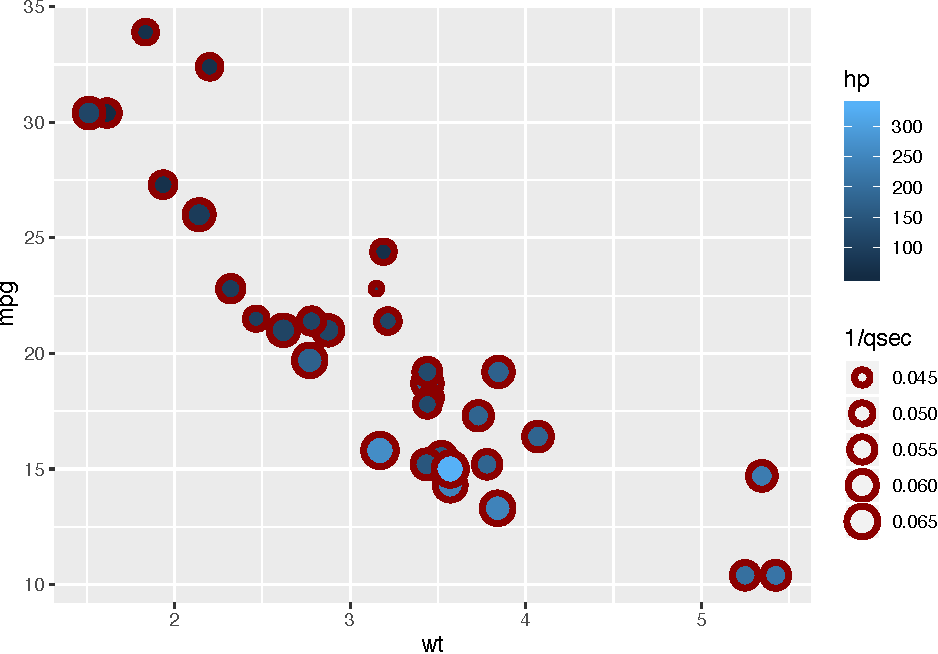
\includegraphics{visualizationwithggplot_files/figure-latex/scatterplot-mapping-1.pdf}

\begin{verbatim}
## Warning in align_plots(plotlist = plots, align = align,
## axis = axis): Complex graphs cannot be vertically
## aligned unless axis parameter is set properly. Placing
## graphs unaligned.
\end{verbatim}

\begin{verbatim}
## Warning in align_plots(plotlist = plots, align = align,
## axis = axis): Graphs cannot be horizontally aligned,
## unless axis parameter set. Placing graphs unaligned.
\end{verbatim}

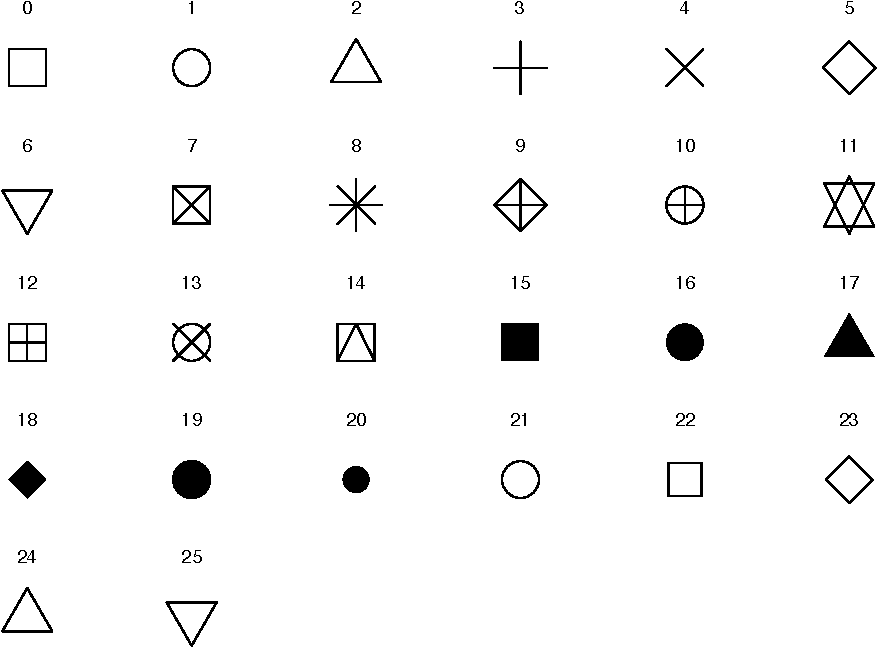
\includegraphics{visualizationwithggplot_files/figure-latex/symbols-1.pdf}

\section{Scatterplot with linear and loess
fit}\label{scatterplot-with-linear-and-loess-fit}

The layers can include geometric elements beyond geom\_point. Perhapts
the most useful geoms to add to a scatterplot is a curve fit. Figure
\ref{fig:scatterplot-smooth} shows a simple scatterplot with two cruve
fits. The loess fit shows a smooth fit that indicates non-linar trends,
and the blue line shows a linear regeression. The loess line highligths
areas in the data that deviate from a linear relationship shown by the
blue line. All three layers inherit the same x and y mapping from the
ggplot base layer.

When building a plot each layer is placed on top of the preceding layer,
such that the last layer lies on top of all the others. With Figure
\ref{fig:scatterplot-smooth}, the points are on the bottom and the light
blue line is on top of the gray loess line.

Table \ref{tab:geoms} shows the full set of possible geometric elements
that can be used to create graphs, the following chapters describe many
of these.

Note the smooth fit geoms include additional settings for the method and
whether the line should include a standard error.

\begin{Shaded}
\begin{Highlighting}[]
\KeywordTok{ggplot}\NormalTok{(}\DataTypeTok{data =}\NormalTok{ mtcars.df, }\KeywordTok{aes}\NormalTok{(}\DataTypeTok{x =}\NormalTok{ wt, }\DataTypeTok{y =}\NormalTok{ mpg)) }\OperatorTok{+}
\StringTok{  }\KeywordTok{geom_point}\NormalTok{(}\DataTypeTok{colour =} \StringTok{"darkblue"}\NormalTok{) }\OperatorTok{+}
\StringTok{  }\KeywordTok{geom_smooth}\NormalTok{(}\DataTypeTok{method =} \StringTok{"loess"}\NormalTok{, }\DataTypeTok{se =} \OtherTok{FALSE}\NormalTok{, }\DataTypeTok{colour =} \StringTok{"darkgrey"}\NormalTok{) }\OperatorTok{+}\StringTok{ }
\StringTok{  }\KeywordTok{geom_smooth}\NormalTok{(}\DataTypeTok{method =} \StringTok{"lm"}\NormalTok{, }\DataTypeTok{fill =} \StringTok{"lightblue"}\NormalTok{)}
\end{Highlighting}
\end{Shaded}

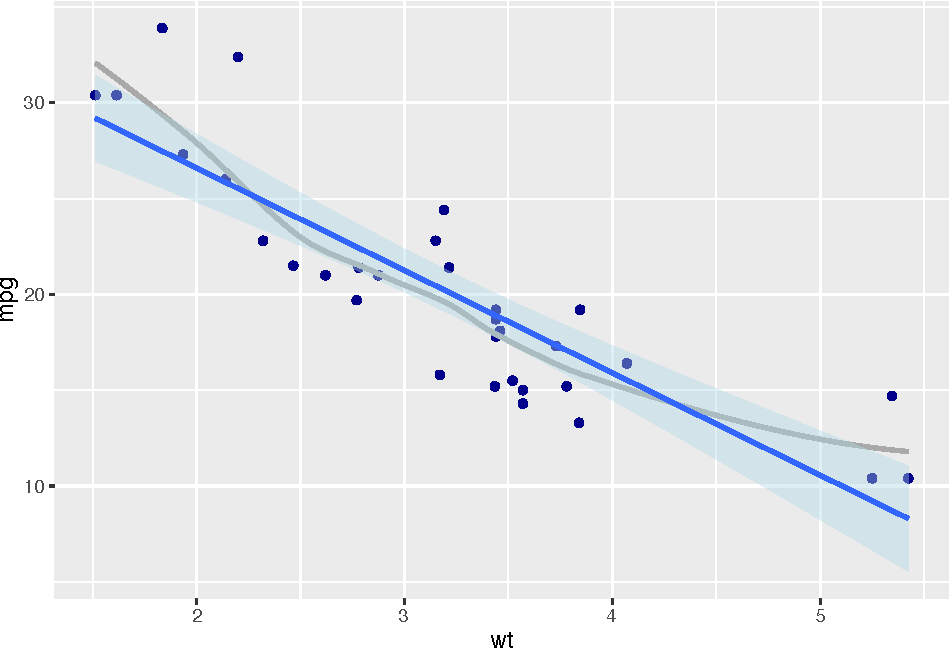
\includegraphics{visualizationwithggplot_files/figure-latex/scatterplot-smooth-1.pdf}

\begin{verbatim}
## Warning: package 'kableExtra' was built under R version
## 3.4.4
\end{verbatim}

\begin{tabular}{l}
\hline
x\\
\hline
geom\_abline\\
\hline
geom\_area\\
\hline
geom\_bar\\
\hline
geom\_bin2d\\
\hline
geom\_blank\\
\hline
geom\_boxplot\\
\hline
geom\_col\\
\hline
geom\_contour\\
\hline
geom\_count\\
\hline
geom\_crossbar\\
\hline
geom\_curve\\
\hline
geom\_density\\
\hline
geom\_density\_2d\\
\hline
geom\_density2d\\
\hline
geom\_dotplot\\
\hline
geom\_errorbar\\
\hline
geom\_errorbarh\\
\hline
geom\_freqpoly\\
\hline
geom\_hex\\
\hline
geom\_histogram\\
\hline
geom\_hline\\
\hline
geom\_jitter\\
\hline
geom\_label\\
\hline
geom\_line\\
\hline
geom\_linerange\\
\hline
geom\_map\\
\hline
geom\_path\\
\hline
geom\_point\\
\hline
geom\_pointrange\\
\hline
geom\_polygon\\
\hline
geom\_qq\\
\hline
geom\_quantile\\
\hline
geom\_raster\\
\hline
geom\_rect\\
\hline
geom\_ribbon\\
\hline
geom\_rug\\
\hline
geom\_segment\\
\hline
geom\_smooth\\
\hline
geom\_spoke\\
\hline
geom\_step\\
\hline
geom\_text\\
\hline
geom\_tile\\
\hline
geom\_violin\\
\hline
geom\_vline\\
\hline
\end{tabular}

\section{Global and local regression}\label{global-and-local-regression}

\begin{Shaded}
\begin{Highlighting}[]
\KeywordTok{ggplot}\NormalTok{(}\DataTypeTok{data =}\NormalTok{ mtcars.df, }\KeywordTok{aes}\NormalTok{(}\DataTypeTok{x =}\NormalTok{ wt, }\DataTypeTok{y =}\NormalTok{ mpg)) }\OperatorTok{+}
\StringTok{    }\KeywordTok{geom_smooth}\NormalTok{(}\DataTypeTok{method =}\NormalTok{ lm, }\DataTypeTok{colour =} \StringTok{"darkgrey"}\NormalTok{, }\DataTypeTok{size =}\NormalTok{ .}\DecValTok{5}\NormalTok{) }\OperatorTok{+}
\StringTok{  }\KeywordTok{geom_point}\NormalTok{(}\KeywordTok{aes}\NormalTok{(}\DataTypeTok{colour =} \KeywordTok{as.factor}\NormalTok{(cyl))) }\OperatorTok{+}
\StringTok{  }\KeywordTok{geom_smooth}\NormalTok{(}\KeywordTok{aes}\NormalTok{(}\DataTypeTok{colour =} \KeywordTok{as.factor}\NormalTok{(cyl)), }\DataTypeTok{method =}\NormalTok{ lm, }\DataTypeTok{se =} \OtherTok{FALSE}\NormalTok{)}
\end{Highlighting}
\end{Shaded}

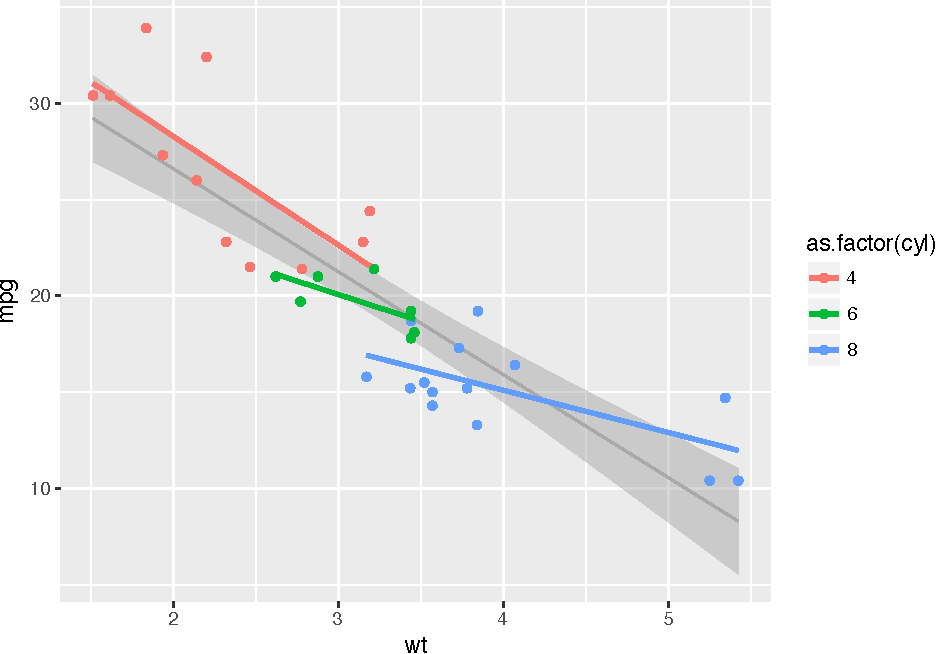
\includegraphics{visualizationwithggplot_files/figure-latex/scatterplot-globallocal-1.pdf}

\section{Quantile regression and other functional
relationships}\label{quantile-regression-and-other-functional-relationships}

Often the question the graph is meant to answer is not about the central
tendency, but about the likelihood of relatively extreme values, such as
the 25th and 75th percentiles.

\begin{Shaded}
\begin{Highlighting}[]
\KeywordTok{ggplot}\NormalTok{(}\DataTypeTok{data =}\NormalTok{ mtcars.df, }\KeywordTok{aes}\NormalTok{(}\DataTypeTok{x =}\NormalTok{ wt, }\DataTypeTok{y =}\NormalTok{ mpg)) }\OperatorTok{+}
\StringTok{    }\KeywordTok{geom_smooth}\NormalTok{(}\DataTypeTok{method =}\NormalTok{ lm, }\DataTypeTok{colour =} \StringTok{"darkgrey"}\NormalTok{, }\DataTypeTok{size =}\NormalTok{ .}\DecValTok{5}\NormalTok{) }\OperatorTok{+}
\StringTok{  }\KeywordTok{geom_point}\NormalTok{() }\OperatorTok{+}
\StringTok{  }\KeywordTok{geom_quantile}\NormalTok{(}\DataTypeTok{quantiles =} \KeywordTok{c}\NormalTok{(.}\DecValTok{25}\NormalTok{, .}\DecValTok{75}\NormalTok{))}
\end{Highlighting}
\end{Shaded}

\begin{verbatim}
## Loading required package: SparseM
\end{verbatim}

\begin{verbatim}
## 
## Attaching package: 'SparseM'
\end{verbatim}

\begin{verbatim}
## The following object is masked from 'package:base':
## 
##     backsolve
\end{verbatim}

\begin{verbatim}
## Smoothing formula not specified. Using: y ~ x
\end{verbatim}

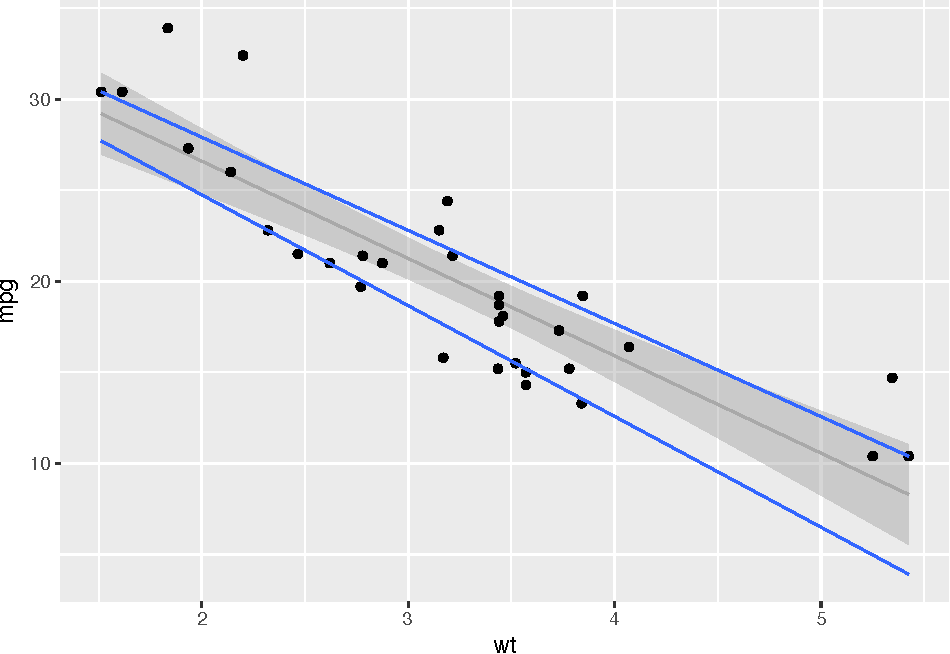
\includegraphics{visualizationwithggplot_files/figure-latex/scatterplot-quantile-1.pdf}

\section{Scatterplot with regression equation and marginal
distributions}\label{scatterplot-with-regression-equation-and-marginal-distributions}

Scatterplot augmented with marginal distributions, regression equation,
and Tufte-inspired range frame.

Marginal distributions show that a 1-D scatterplot is a histogram and
that a 2-d histogram is a scatterplot. Chapter \ref{Distribution}
describes such plots in detail.

Chapter \ref{Polishing} shows how to add annotations, such as the
equation.

Derived from:
\url{http://t-redactyl.io/blog/2016/05/creating-plots-in-r-using-ggplot2-part-11-linear-regression-plots.html}

\begin{Shaded}
\begin{Highlighting}[]
\KeywordTok{library}\NormalTok{(ggthemes)}
\KeywordTok{library}\NormalTok{(ggExtra) }\CommentTok{# For marginal histograms}
\end{Highlighting}
\end{Shaded}

\begin{verbatim}
## Warning: package 'ggExtra' was built under R version
## 3.4.4
\end{verbatim}

\begin{Shaded}
\begin{Highlighting}[]
\NormalTok{equation =}\StringTok{ }\ControlFlowTok{function}\NormalTok{(x) \{}
\NormalTok{  lm_coef <-}\StringTok{ }\KeywordTok{list}\NormalTok{(}\DataTypeTok{a =} \KeywordTok{round}\NormalTok{(}\KeywordTok{coef}\NormalTok{(x)[}\DecValTok{1}\NormalTok{], }\DataTypeTok{digits =} \DecValTok{2}\NormalTok{),}
                  \DataTypeTok{b =} \KeywordTok{round}\NormalTok{(}\KeywordTok{coef}\NormalTok{(x)[}\DecValTok{2}\NormalTok{], }\DataTypeTok{digits =} \DecValTok{2}\NormalTok{),}
                  \DataTypeTok{r2 =} \KeywordTok{round}\NormalTok{(}\KeywordTok{summary}\NormalTok{(x)}\OperatorTok{$}\NormalTok{r.squared, }\DataTypeTok{digits =} \DecValTok{2}\NormalTok{));}
\NormalTok{  lm_eq <-}\StringTok{ }\KeywordTok{substitute}\NormalTok{(}\KeywordTok{italic}\NormalTok{(y) }\OperatorTok{==}\StringTok{ }\NormalTok{a }\OperatorTok{+}\StringTok{ }\NormalTok{b }\OperatorTok\StringTok{ }\KeywordTok{italic}\NormalTok{(x)}\OperatorTok{*}\StringTok{","}\OperatorTok{~}\ErrorTok{~}\KeywordTok{italic}\NormalTok{(R)}\OperatorTok{^}\DecValTok{2}\OperatorTok{~}\StringTok{"="}\OperatorTok{~}\NormalTok{r2,lm_coef)}
  \KeywordTok{as.character}\NormalTok{(}\KeywordTok{as.expression}\NormalTok{(lm_eq));                 }
\NormalTok{\}}

\NormalTok{mtcars.df =}\StringTok{ }\NormalTok{mtcars}
\NormalTok{fit =}\StringTok{ }\KeywordTok{lm}\NormalTok{(mpg}\OperatorTok{~}\NormalTok{wt, }\DataTypeTok{data =}\NormalTok{ mtcars.df)}

\NormalTok{p =}\StringTok{ }\KeywordTok{ggplot}\NormalTok{(mtcars.df, }\KeywordTok{aes}\NormalTok{(}\DataTypeTok{x=}\NormalTok{wt, }\DataTypeTok{y=}\NormalTok{mpg)) }\OperatorTok{+}\StringTok{ }
\StringTok{  }\KeywordTok{geom_point}\NormalTok{(}\DataTypeTok{colour =} \StringTok{"darkblue"}\NormalTok{) }\OperatorTok{+}\StringTok{ }
\StringTok{  }\KeywordTok{geom_smooth}\NormalTok{(}\DataTypeTok{method=}\NormalTok{lm, }\DataTypeTok{se=}\OtherTok{FALSE}\NormalTok{) }\OperatorTok{+}
\StringTok{  }\KeywordTok{annotate}\NormalTok{(}\StringTok{"text"}\NormalTok{, }\DataTypeTok{x =} \DecValTok{4}\NormalTok{, }\DataTypeTok{y =} \DecValTok{30}\NormalTok{, }\DataTypeTok{label =} \KeywordTok{equation}\NormalTok{(fit), }\DataTypeTok{parse =} \OtherTok{TRUE}\NormalTok{) }\OperatorTok{+}
\StringTok{  }\KeywordTok{geom_rangeframe}\NormalTok{() }\OperatorTok{+}\StringTok{ }\CommentTok{# Requires ggthemes }
\StringTok{  }\KeywordTok{theme_minimal}\NormalTok{()}

\NormalTok{p =}\StringTok{ }\KeywordTok{ggMarginal}\NormalTok{(p, }\DataTypeTok{type =} \StringTok{"histogram"}\NormalTok{)}
\NormalTok{p}
\end{Highlighting}
\end{Shaded}

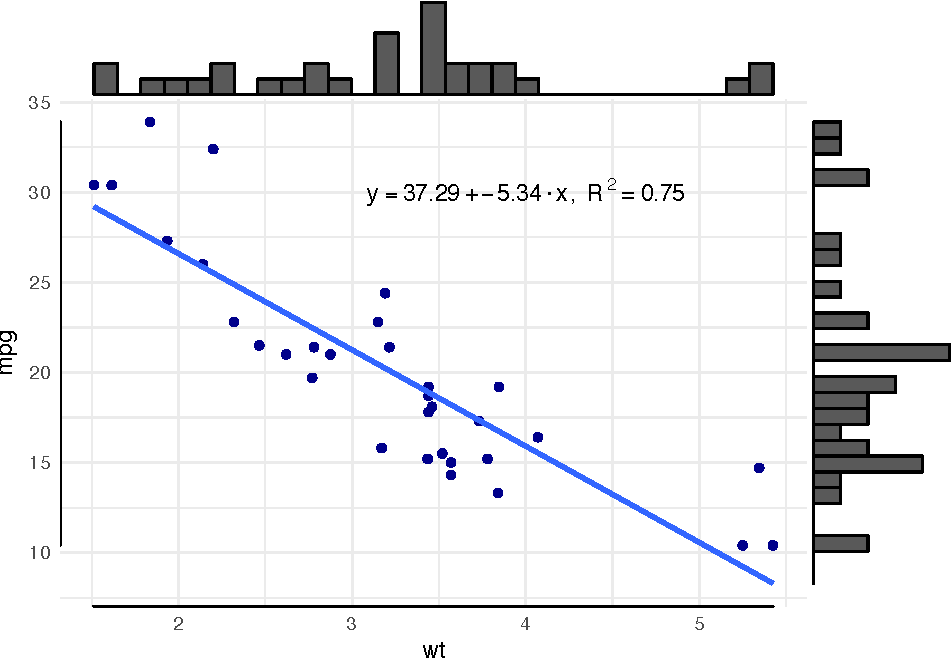
\includegraphics{visualizationwithggplot_files/figure-latex/scatterplot-marginal-1.pdf}

\section{Categorical scatterplot}\label{categorical-scatterplot}

\begin{Shaded}
\begin{Highlighting}[]
\NormalTok{mtcars.df =}\StringTok{ }\NormalTok{mtcars}
\NormalTok{mtcars.df}\OperatorTok{$}\NormalTok{gear =}\StringTok{ }\KeywordTok{as.factor}\NormalTok{(mtcars.df}\OperatorTok{$}\NormalTok{gear)}
\NormalTok{mtcars.df}\OperatorTok{$}\NormalTok{am =}\StringTok{ }\KeywordTok{as.factor}\NormalTok{(mtcars.df}\OperatorTok{$}\NormalTok{am)}

\KeywordTok{ggplot}\NormalTok{(mtcars.df, }\KeywordTok{aes}\NormalTok{(gear, am)) }\OperatorTok{+}\StringTok{ }
\StringTok{  }\KeywordTok{geom_count}\NormalTok{()}
\end{Highlighting}
\end{Shaded}

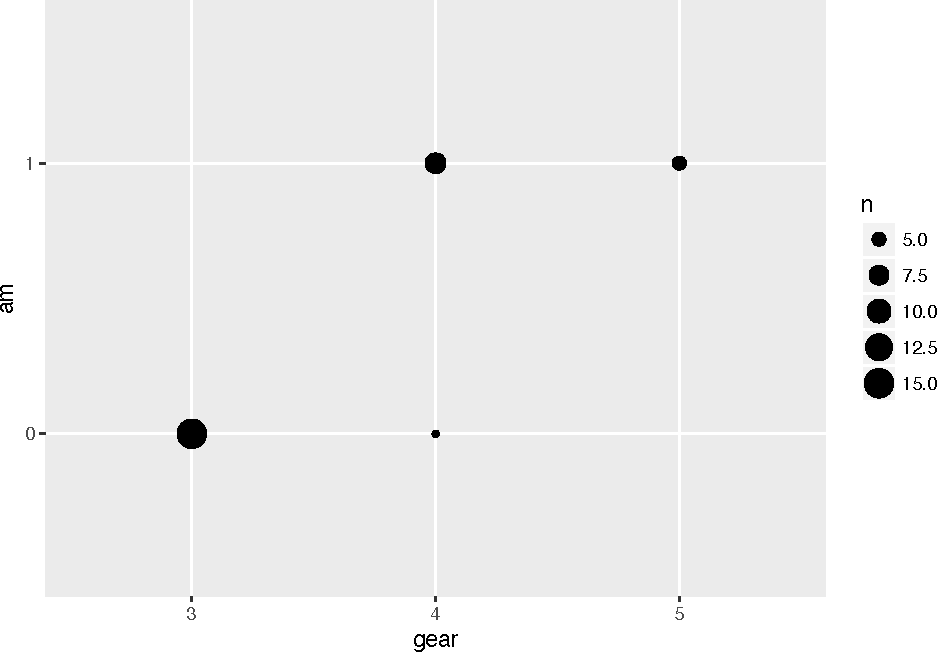
\includegraphics{visualizationwithggplot_files/figure-latex/scatterplot-categorical-1.pdf}

\begin{Shaded}
\begin{Highlighting}[]
 \KeywordTok{ggplot}\NormalTok{(mtcars.df, }\KeywordTok{aes}\NormalTok{(gear, am)) }\OperatorTok{+}\StringTok{ }
\StringTok{  }\KeywordTok{geom_jitter}\NormalTok{(}\DataTypeTok{width =} \FloatTok{0.075}\NormalTok{, }\DataTypeTok{height =} \FloatTok{0.075}\NormalTok{) }
\end{Highlighting}
\end{Shaded}

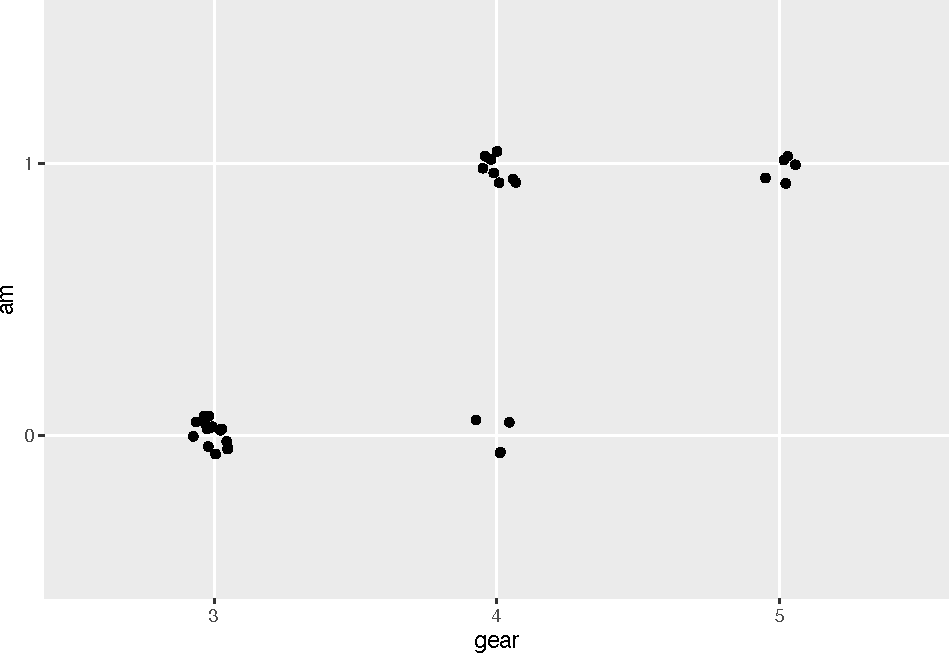
\includegraphics{visualizationwithggplot_files/figure-latex/scatterplot-categorical-2.pdf}

\begin{Shaded}
\begin{Highlighting}[]
\NormalTok{s.mtcars.df =}\StringTok{ }\NormalTok{mtcars.df }\OperatorTok\StringTok{ }\KeywordTok{group_by}\NormalTok{(gear, am) }\OperatorTok\StringTok{ }\KeywordTok{summarise}\NormalTok{(}\DataTypeTok{count =} \KeywordTok{n}\NormalTok{())}

\KeywordTok{ggplot}\NormalTok{(s.mtcars.df, }\KeywordTok{aes}\NormalTok{(gear, am)) }\OperatorTok{+}\StringTok{ }
\StringTok{  }\KeywordTok{geom_tile}\NormalTok{(}\KeywordTok{aes}\NormalTok{(}\DataTypeTok{fill =}\NormalTok{ count))}
\end{Highlighting}
\end{Shaded}

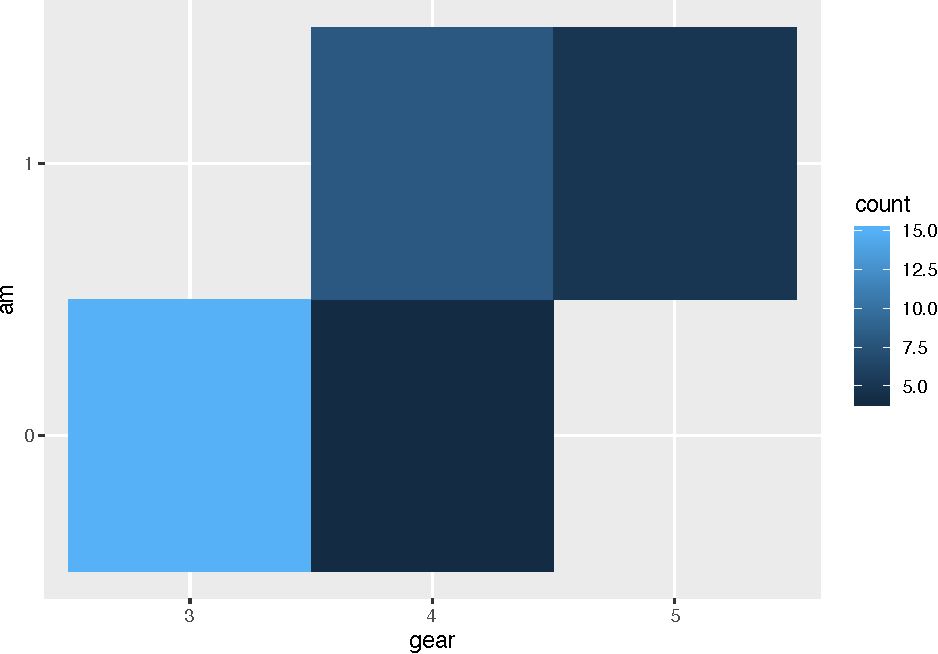
\includegraphics{visualizationwithggplot_files/figure-latex/scatterplot-categorical-3.pdf}

\section{Table lens}\label{table-lens}

Table lens serves a similar purpose to the scatterplot but might be more
familiar and focusses attention on individual variables and individual
cases. Chapter \ref{Tables} provides more detail on this technique.

\hypertarget{htmlwidget-8b255151ac9d79a9c02d}{}

\section{Scatterplot with overplotting
mitigation}\label{scatterplot-with-overplotting-mitigation}

\begin{Shaded}
\begin{Highlighting}[]
\NormalTok{diamonds.df =}\StringTok{ }\NormalTok{diamonds}

\KeywordTok{ggplot}\NormalTok{(diamonds.df, }\KeywordTok{aes}\NormalTok{(carat, price)) }\OperatorTok{+}
\StringTok{  }\KeywordTok{geom_point}\NormalTok{()}
\end{Highlighting}
\end{Shaded}

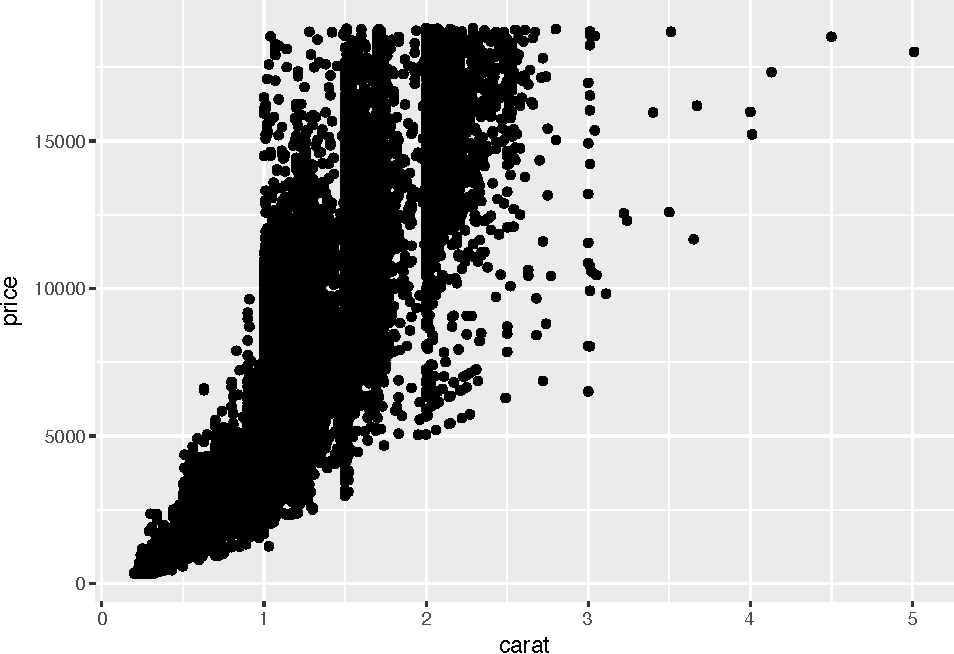
\includegraphics{visualizationwithggplot_files/figure-latex/scatterplot-overplot-1.pdf}

\begin{Shaded}
\begin{Highlighting}[]
\KeywordTok{ggplot}\NormalTok{(diamonds.df, }\KeywordTok{aes}\NormalTok{(carat, price)) }\OperatorTok{+}
\StringTok{  }\KeywordTok{geom_point}\NormalTok{(}\DataTypeTok{size =}\NormalTok{ .}\DecValTok{1}\NormalTok{)}
\end{Highlighting}
\end{Shaded}

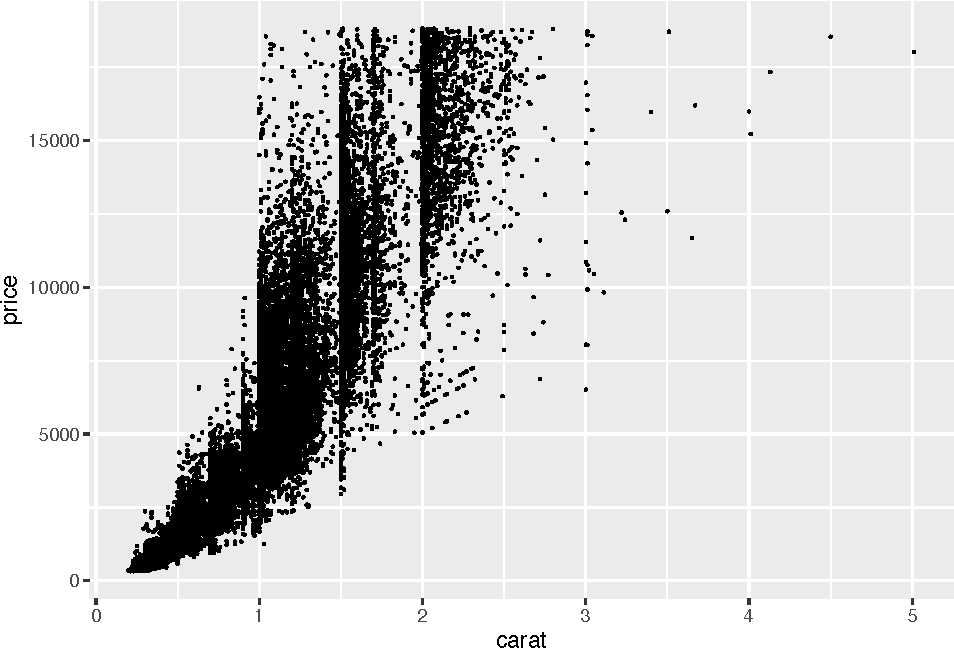
\includegraphics{visualizationwithggplot_files/figure-latex/scatterplot-overplot-2.pdf}

\begin{Shaded}
\begin{Highlighting}[]
\KeywordTok{ggplot}\NormalTok{(diamonds.df, }\KeywordTok{aes}\NormalTok{(carat, price)) }\OperatorTok{+}
\StringTok{  }\KeywordTok{geom_point}\NormalTok{(}\DataTypeTok{size =}\NormalTok{ .}\DecValTok{3}\NormalTok{, }\DataTypeTok{shape =} \DecValTok{21}\NormalTok{)}
\end{Highlighting}
\end{Shaded}

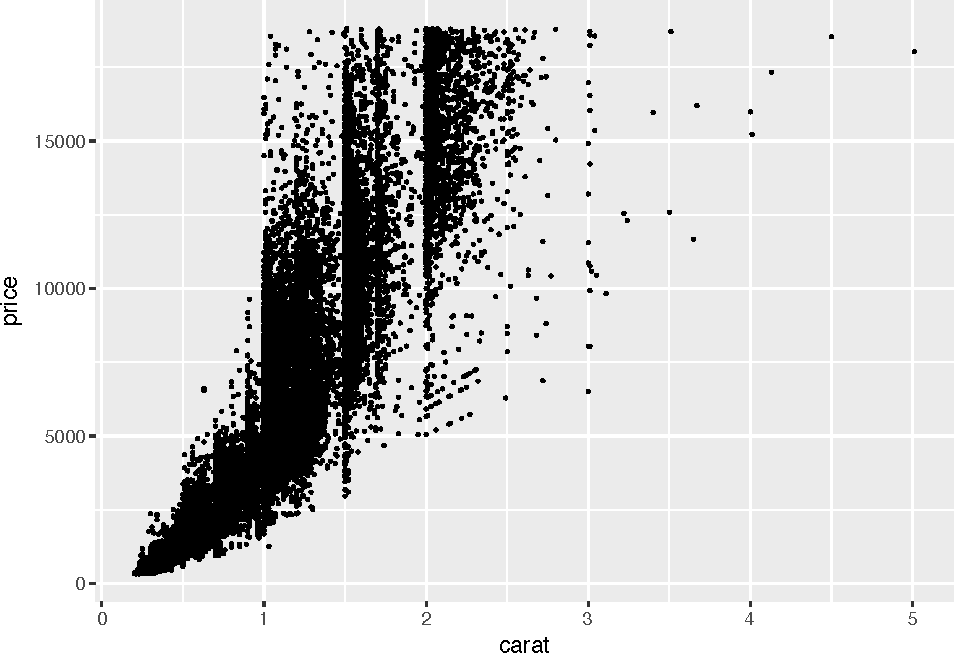
\includegraphics{visualizationwithggplot_files/figure-latex/scatterplot-overplot-3.pdf}

\begin{Shaded}
\begin{Highlighting}[]
\KeywordTok{ggplot}\NormalTok{(diamonds.df, }\KeywordTok{aes}\NormalTok{(carat, price)) }\OperatorTok{+}
\StringTok{  }\KeywordTok{geom_point}\NormalTok{(}\DataTypeTok{size =}\NormalTok{ .}\DecValTok{3}\NormalTok{, }\DataTypeTok{shape =} \DecValTok{21}\NormalTok{, }\DataTypeTok{alpha =}\NormalTok{ .}\DecValTok{3}\NormalTok{)}
\end{Highlighting}
\end{Shaded}

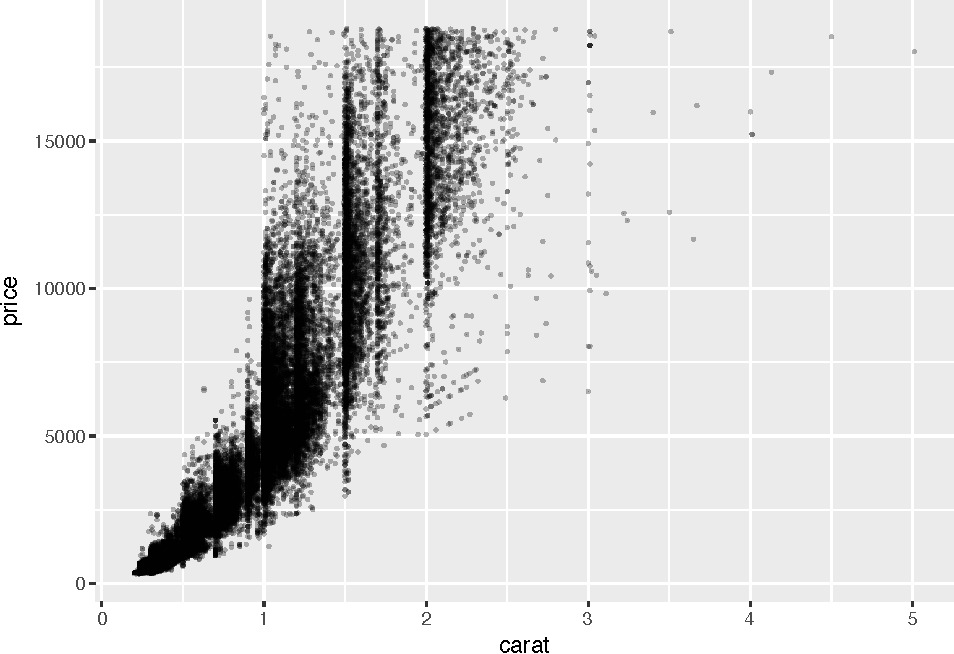
\includegraphics{visualizationwithggplot_files/figure-latex/scatterplot-overplot-4.pdf}

\begin{Shaded}
\begin{Highlighting}[]
\KeywordTok{ggplot}\NormalTok{(diamonds.df }\OperatorTok\StringTok{ }\KeywordTok{sample_n}\NormalTok{(}\DecValTok{10000}\NormalTok{), }\KeywordTok{aes}\NormalTok{(carat, price)) }\OperatorTok{+}
\StringTok{  }\KeywordTok{geom_point}\NormalTok{(}\DataTypeTok{size =}\NormalTok{ .}\DecValTok{3}\NormalTok{, }\DataTypeTok{shape =} \DecValTok{21}\NormalTok{, }\DataTypeTok{alpha =}\NormalTok{ .}\DecValTok{3}\NormalTok{)}
\end{Highlighting}
\end{Shaded}

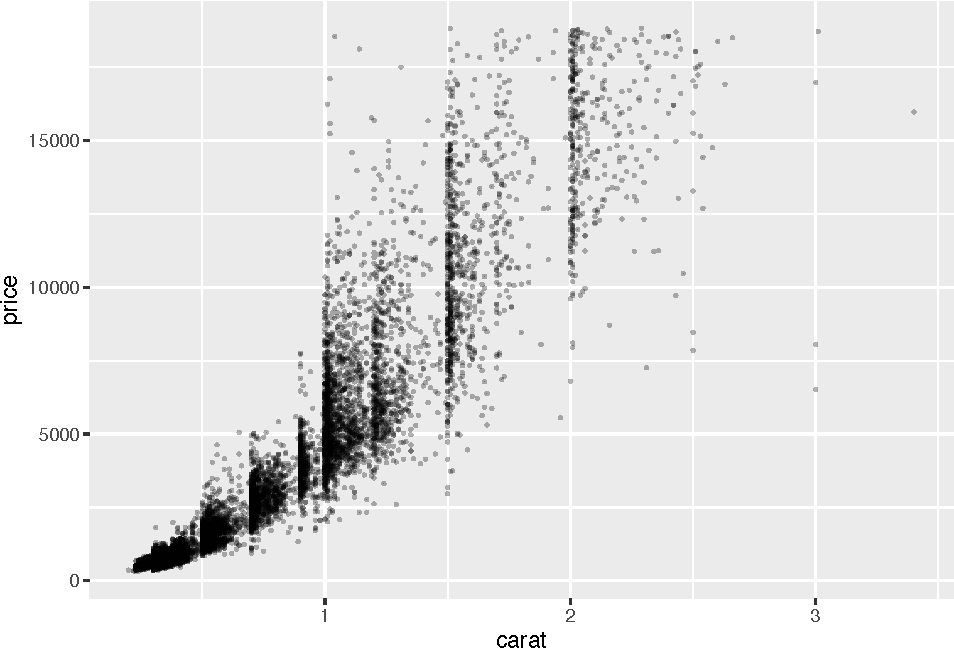
\includegraphics{visualizationwithggplot_files/figure-latex/scatterplot-overplot-5.pdf}

\begin{Shaded}
\begin{Highlighting}[]
\KeywordTok{ggplot}\NormalTok{(diamonds.df, }\KeywordTok{aes}\NormalTok{(}\KeywordTok{log}\NormalTok{(carat), }\KeywordTok{log}\NormalTok{(price))) }\OperatorTok{+}
\StringTok{  }\KeywordTok{geom_point}\NormalTok{(}\DataTypeTok{size =}\NormalTok{ .}\DecValTok{3}\NormalTok{, }\DataTypeTok{shape =} \DecValTok{21}\NormalTok{, }\DataTypeTok{alpha =}\NormalTok{ .}\DecValTok{3}\NormalTok{)}
\end{Highlighting}
\end{Shaded}

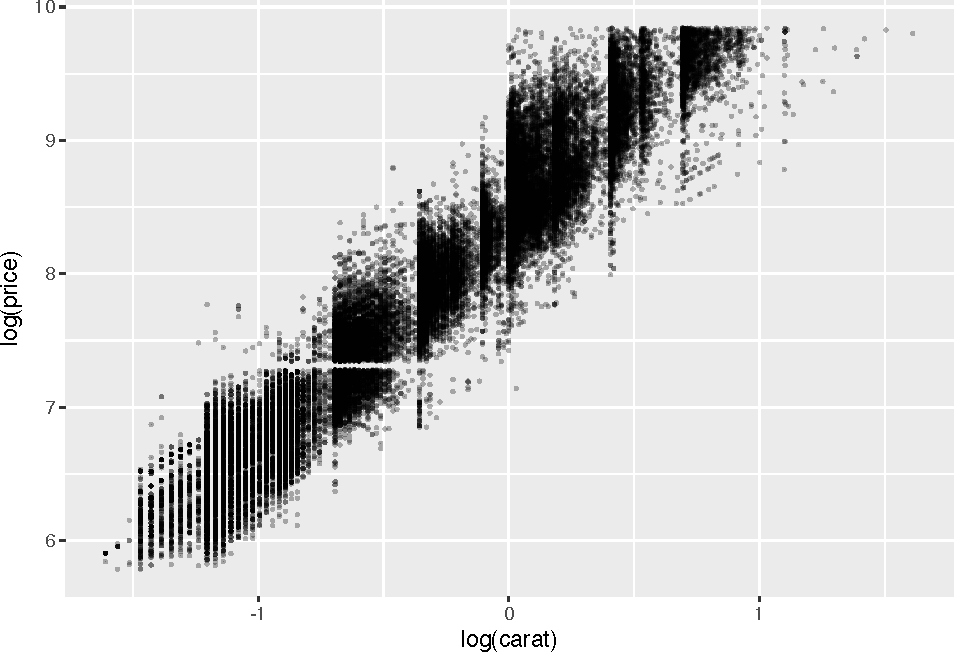
\includegraphics{visualizationwithggplot_files/figure-latex/scatterplot-overplot-6.pdf}

\begin{Shaded}
\begin{Highlighting}[]
\KeywordTok{ggplot}\NormalTok{(diamonds.df, }\KeywordTok{aes}\NormalTok{(}\KeywordTok{log}\NormalTok{(carat), }\KeywordTok{log}\NormalTok{(price))) }\OperatorTok{+}
\StringTok{  }\KeywordTok{geom_count}\NormalTok{(}\DataTypeTok{show.legend=}\NormalTok{F, }\DataTypeTok{alpha =}\NormalTok{.}\DecValTok{3}\NormalTok{, }\DataTypeTok{shape =}\DecValTok{21}\NormalTok{)}
\end{Highlighting}
\end{Shaded}

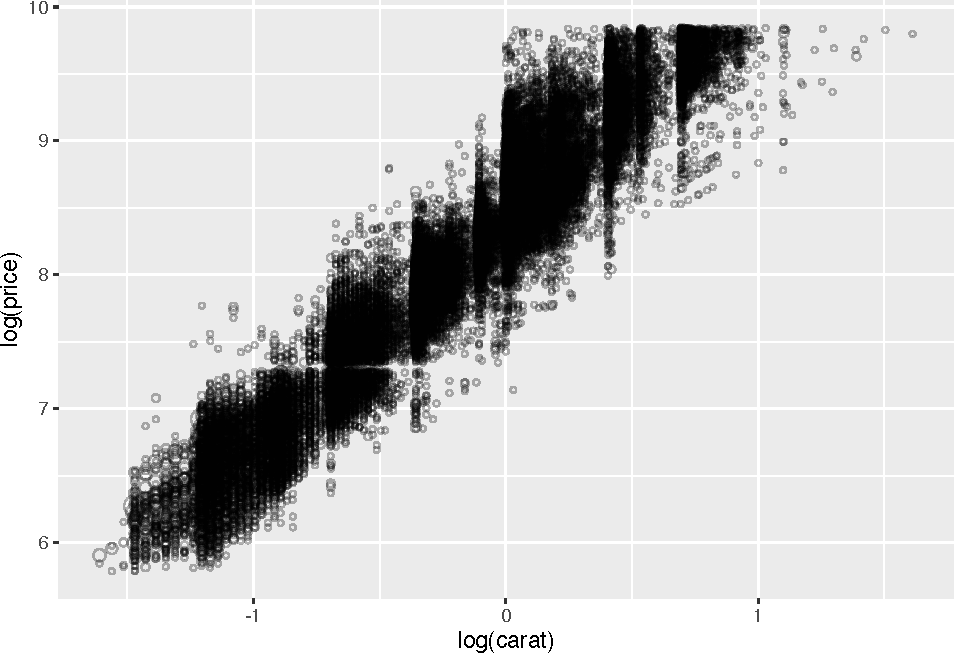
\includegraphics{visualizationwithggplot_files/figure-latex/scatterplot-overplot-7.pdf}

\begin{Shaded}
\begin{Highlighting}[]
\KeywordTok{ggplot}\NormalTok{(}\DataTypeTok{data =}\NormalTok{ mtcars.df, }\KeywordTok{aes}\NormalTok{( }\DataTypeTok{x =}\NormalTok{ disp, }\DataTypeTok{y =}\NormalTok{ hp)) }\OperatorTok{+}
\StringTok{  }\KeywordTok{geom_point}\NormalTok{(}\DataTypeTok{colour =} \StringTok{"grey40"}\NormalTok{, }\DataTypeTok{shape =} \DecValTok{21}\NormalTok{)}\OperatorTok{+}
\StringTok{  }\KeywordTok{geom_smooth}\NormalTok{(}\DataTypeTok{method =}\NormalTok{ loess, }\DataTypeTok{colour =} \StringTok{"grey40"}\NormalTok{)}\OperatorTok{+}
\StringTok{  }\KeywordTok{geom_smooth}\NormalTok{(}\DataTypeTok{method =}\NormalTok{ lm, }\DataTypeTok{se =} \OtherTok{FALSE}\NormalTok{, }\DataTypeTok{size =}\NormalTok{ .}\DecValTok{75}\NormalTok{) }\OperatorTok{+}
\StringTok{    }\KeywordTok{geom_smooth}\NormalTok{(}\KeywordTok{aes}\NormalTok{(}\DataTypeTok{colour =} \KeywordTok{factor}\NormalTok{(cyl)), }
        \DataTypeTok{method =}\NormalTok{ lm, }\DataTypeTok{se =} \OtherTok{FALSE}\NormalTok{, }\DataTypeTok{size =} \FloatTok{1.5}\NormalTok{)}
\end{Highlighting}
\end{Shaded}

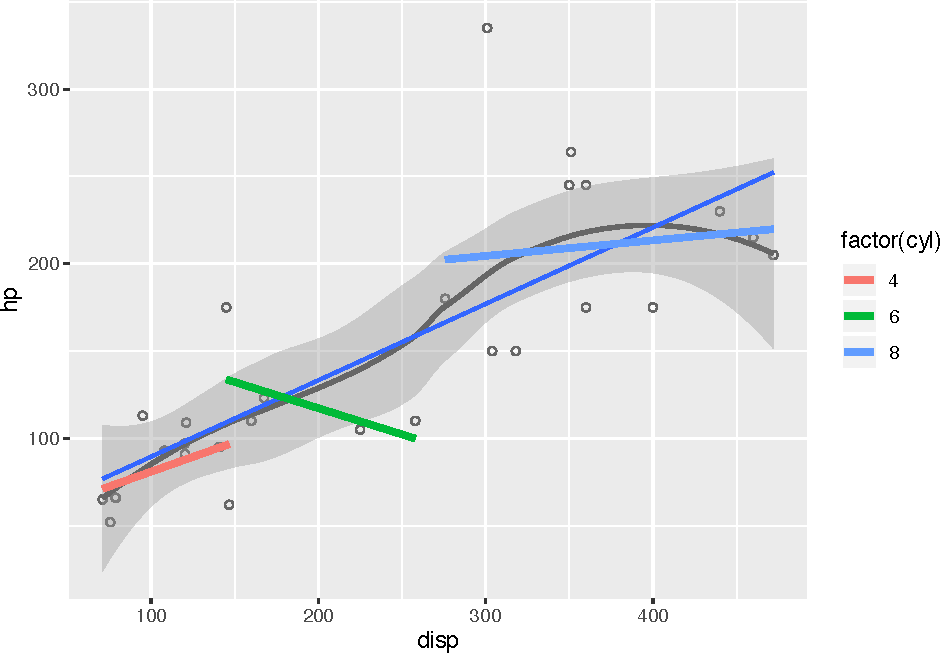
\includegraphics{visualizationwithggplot_files/figure-latex/scatterplot-overplot-8.pdf}

\section{A matrix of scatterplots}\label{a-matrix-of-scatterplots}

\begin{verbatim}
##  [1] "mpg"  "cyl"  "disp" "hp"   "drat" "wt"   "qsec"
##  [8] "vs"   "am"   "gear" "carb"
\end{verbatim}

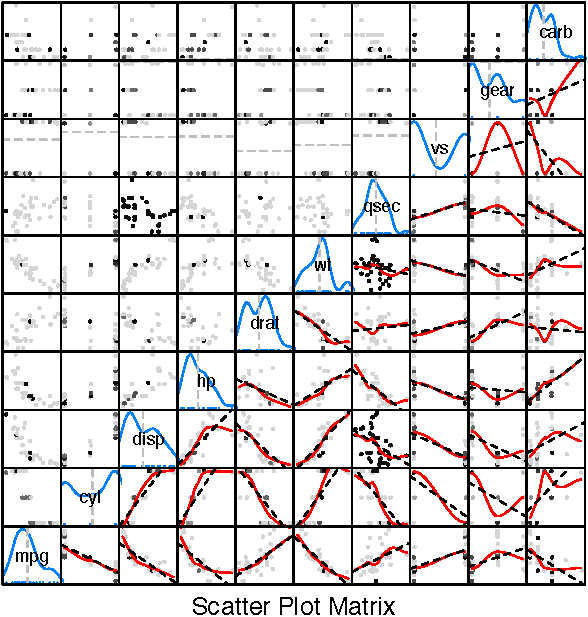
\includegraphics{visualizationwithggplot_files/figure-latex/scatterplot-matrix-1.pdf}

\cleardoublepage 

\chapter{Distribution--histograms and density plots}\label{Distribution}

\begin{Shaded}
\begin{Highlighting}[]
\KeywordTok{library}\NormalTok{(tidyverse)}
\KeywordTok{library}\NormalTok{(HistData)}
\end{Highlighting}
\end{Shaded}

Seeing the smooth and rough of data bins or binwidth, default number of
bins is 30

\section{Histograms and bin choice}\label{histograms-and-bin-choice}

\begin{Shaded}
\begin{Highlighting}[]
\NormalTok{h10.plot =}\StringTok{ }\KeywordTok{ggplot}\NormalTok{(}\DataTypeTok{data =}\NormalTok{ diamonds.df, }\KeywordTok{aes}\NormalTok{(price)) }\OperatorTok{+}\StringTok{ }
\StringTok{  }\KeywordTok{geom_histogram}\NormalTok{(}\DataTypeTok{bins =} \DecValTok{10}\NormalTok{) }

\NormalTok{h30.plot =}\StringTok{ }\KeywordTok{ggplot}\NormalTok{(}\DataTypeTok{data =}\NormalTok{ diamonds.df, }\KeywordTok{aes}\NormalTok{(price)) }\OperatorTok{+}\StringTok{ }
\StringTok{  }\KeywordTok{geom_histogram}\NormalTok{(}\DataTypeTok{bins =} \DecValTok{30}\NormalTok{) }

\NormalTok{h80.plot =}\StringTok{ }\KeywordTok{ggplot}\NormalTok{(}\DataTypeTok{data =}\NormalTok{ diamonds.df, }\KeywordTok{aes}\NormalTok{(price)) }\OperatorTok{+}\StringTok{ }
\StringTok{  }\KeywordTok{geom_histogram}\NormalTok{(}\DataTypeTok{bins =} \DecValTok{80}\NormalTok{) }

\KeywordTok{ggarrange}\NormalTok{(h10.plot, h30.plot, h80.plot,}
    \DataTypeTok{nrow=}\DecValTok{1}\NormalTok{, }\DataTypeTok{ncol =} \DecValTok{3}\NormalTok{, }\DataTypeTok{align =} \StringTok{"h"}\NormalTok{)}
\end{Highlighting}
\end{Shaded}

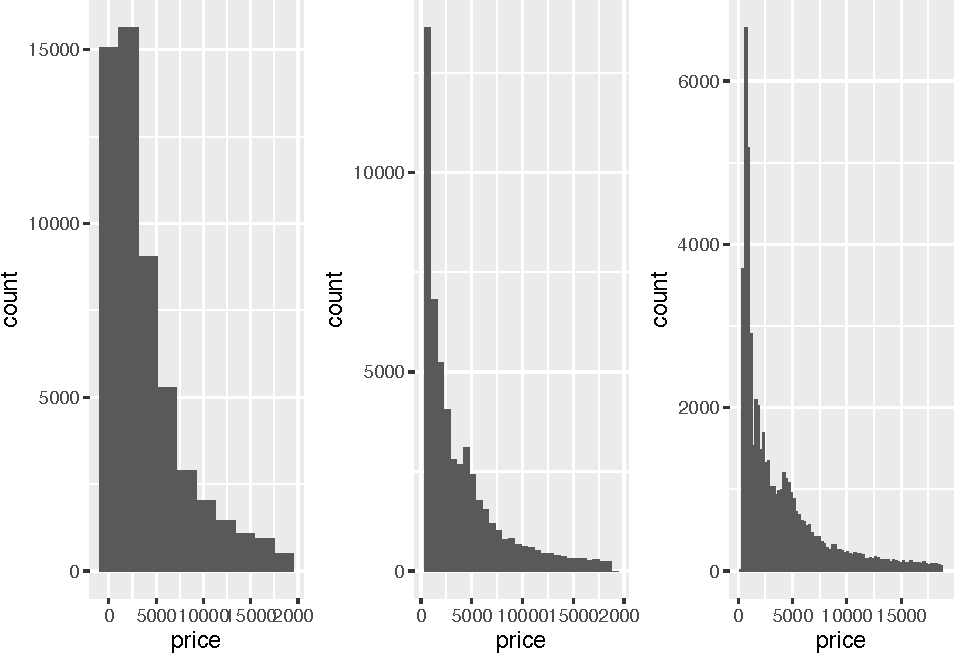
\includegraphics{visualizationwithggplot_files/figure-latex/histogram-bin-1.pdf}

Density as abstraction and model

Adjust is a multiplier on the default kernel bandwidth and so 1
represents the default \#\# Density and kernel adjustment

\begin{Shaded}
\begin{Highlighting}[]
\NormalTok{a10.plot =}\StringTok{ }\KeywordTok{ggplot}\NormalTok{(}\DataTypeTok{data =}\NormalTok{ diamonds.df, }\KeywordTok{aes}\NormalTok{(price)) }\OperatorTok{+}\StringTok{ }
\StringTok{  }\KeywordTok{geom_density}\NormalTok{(}\DataTypeTok{adjust =} \DecValTok{10}\NormalTok{) }

\NormalTok{a1.plot =}\StringTok{ }\KeywordTok{ggplot}\NormalTok{(}\DataTypeTok{data =}\NormalTok{ diamonds.df, }\KeywordTok{aes}\NormalTok{(price)) }\OperatorTok{+}\StringTok{ }
\StringTok{  }\KeywordTok{geom_density}\NormalTok{(}\DataTypeTok{adjust =} \DecValTok{1}\NormalTok{) }

\NormalTok{a01.plot =}\StringTok{ }\KeywordTok{ggplot}\NormalTok{(}\DataTypeTok{data =}\NormalTok{ diamonds.df, }\KeywordTok{aes}\NormalTok{(price)) }\OperatorTok{+}\StringTok{ }
\StringTok{  }\KeywordTok{geom_density}\NormalTok{(}\DataTypeTok{adjust  =} \FloatTok{0.1}\NormalTok{) }

\KeywordTok{ggarrange}\NormalTok{(a10.plot, a1.plot, a01.plot,}
    \DataTypeTok{nrow=}\DecValTok{1}\NormalTok{, }\DataTypeTok{ncol =} \DecValTok{3}\NormalTok{, }\DataTypeTok{align =} \StringTok{"h"}\NormalTok{)}
\end{Highlighting}
\end{Shaded}

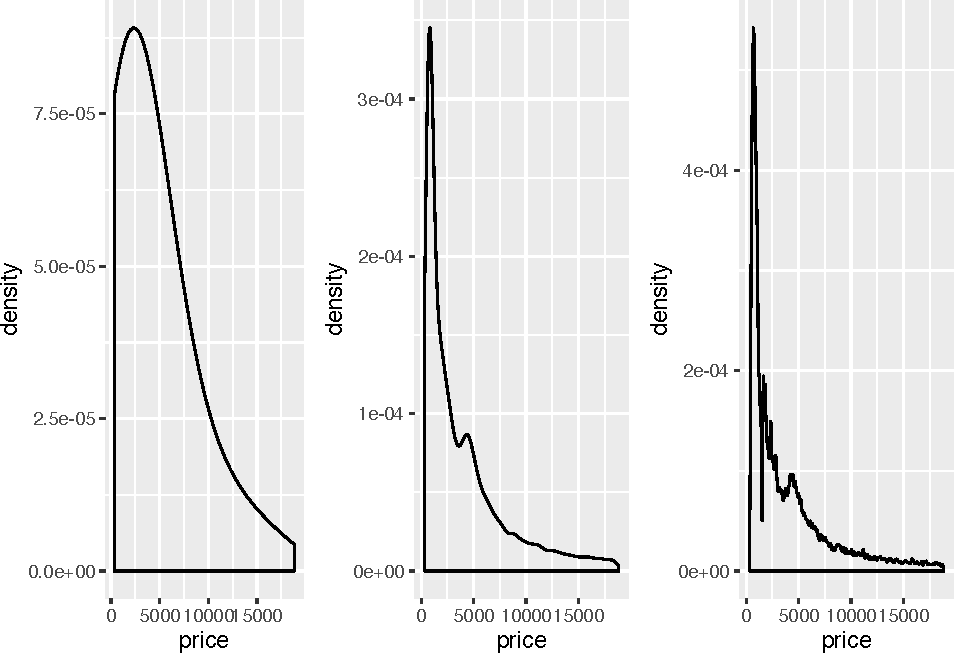
\includegraphics{visualizationwithggplot_files/figure-latex/density-adjust-1.pdf}

\section{Histogram percentage rather than
count}\label{histogram-percentage-rather-than-count}

\begin{Shaded}
\begin{Highlighting}[]
\KeywordTok{ggplot}\NormalTok{(mtcars.df , }\KeywordTok{aes}\NormalTok{(}\DataTypeTok{x =}\NormalTok{ cyl)) }\OperatorTok{+}\StringTok{ }
\StringTok{    }\KeywordTok{geom_bar}\NormalTok{(}\KeywordTok{aes}\NormalTok{(}\DataTypeTok{y =}\NormalTok{ (..count..)}\OperatorTok{/}\KeywordTok{sum}\NormalTok{(..count..))) }\OperatorTok{+}\StringTok{ }
\StringTok{    }\KeywordTok{scale_y_continuous}\NormalTok{(}\DataTypeTok{labels =}\NormalTok{ percent)}
\end{Highlighting}
\end{Shaded}

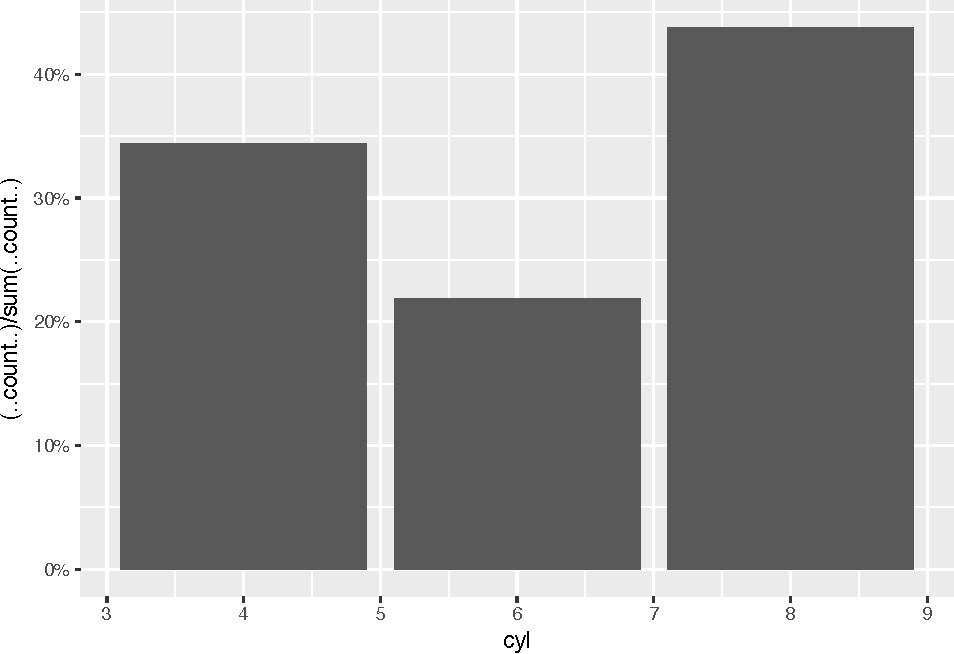
\includegraphics{visualizationwithggplot_files/figure-latex/histogram-percentage-1.pdf}

\section{Histogram, density overlay, and normal
overlay}\label{histogram-density-overlay-and-normal-overlay}

\section{Cummulative density}\label{cummulative-density}

\begin{Shaded}
\begin{Highlighting}[]
\KeywordTok{ggplot}\NormalTok{(diamonds.df, }\KeywordTok{aes}\NormalTok{(price, }\DataTypeTok{colour =}\NormalTok{ cut)) }\OperatorTok{+}\StringTok{ }
\StringTok{  }\KeywordTok{stat_ecdf}\NormalTok{(}\DataTypeTok{geom =} \StringTok{"step"}\NormalTok{)}
\end{Highlighting}
\end{Shaded}

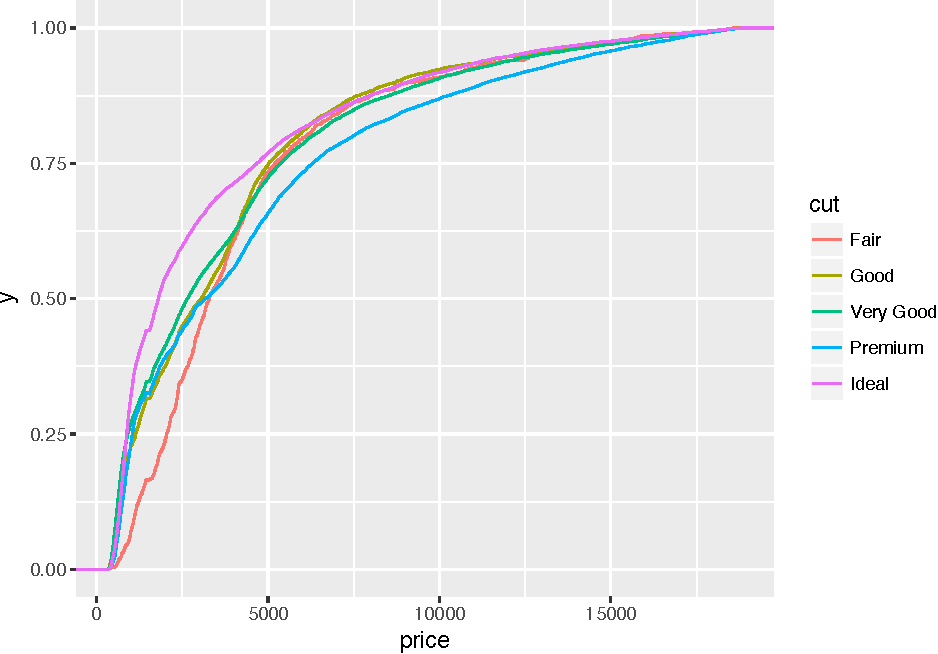
\includegraphics{visualizationwithggplot_files/figure-latex/unnamed-chunk-5-1.pdf}

\section{Quantile-quantle plot}\label{quantile-quantle-plot}

Plots quantiles of sample as a function of the quantiles of the
theoretical distribution.

\begin{Shaded}
\begin{Highlighting}[]
\NormalTok{diamonds.df =}\StringTok{ }\NormalTok{diamonds}

\KeywordTok{ggplot}\NormalTok{(diamonds.df, }\KeywordTok{aes}\NormalTok{(}\DataTypeTok{sample =}\NormalTok{ price)) }\OperatorTok{+}\StringTok{ }
\StringTok{  }\KeywordTok{geom_qq}\NormalTok{(}\DataTypeTok{distribution =}\NormalTok{ qlnorm) }\OperatorTok{+}
\StringTok{  }\KeywordTok{geom_abline}\NormalTok{(}\DataTypeTok{intercept =} \KeywordTok{mean}\NormalTok{(diamonds.df}\OperatorTok{$}\NormalTok{price), }\DataTypeTok{slope =} \KeywordTok{sd}\NormalTok{(diamonds.df}\OperatorTok{$}\NormalTok{price))}
\end{Highlighting}
\end{Shaded}

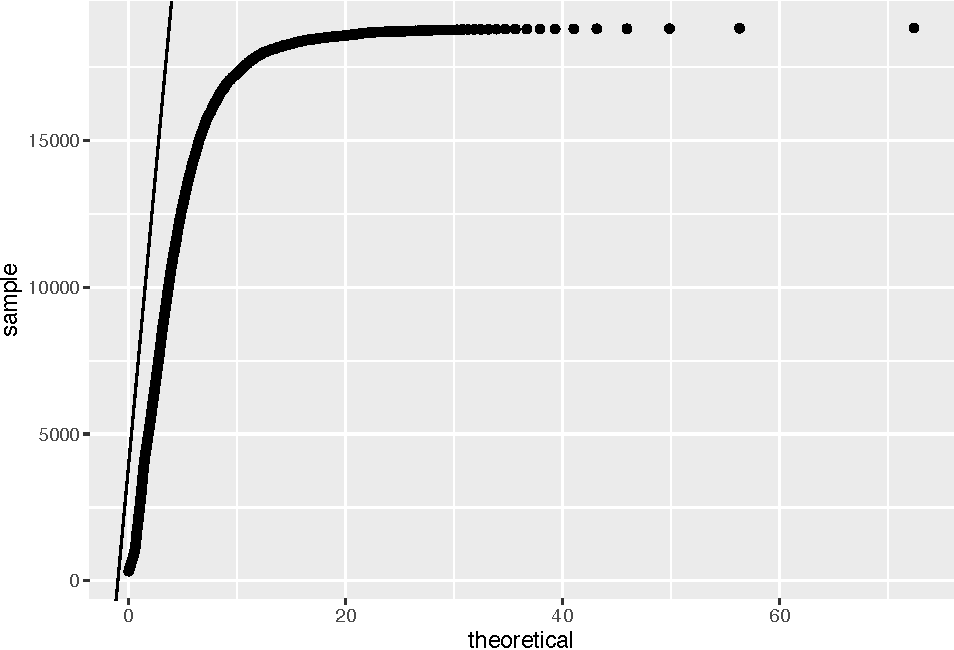
\includegraphics{visualizationwithggplot_files/figure-latex/qqplot-1.pdf}

\section{Cummulative density}\label{cummulative-density-1}

\begin{Shaded}
\begin{Highlighting}[]
\KeywordTok{ggplot}\NormalTok{(diamonds.df, }\KeywordTok{aes}\NormalTok{(price, }\DataTypeTok{colour =}\NormalTok{ cut)) }\OperatorTok{+}\StringTok{ }
\StringTok{  }\KeywordTok{stat_ecdf}\NormalTok{(}\DataTypeTok{geom =} \StringTok{"step"}\NormalTok{)}
\end{Highlighting}
\end{Shaded}

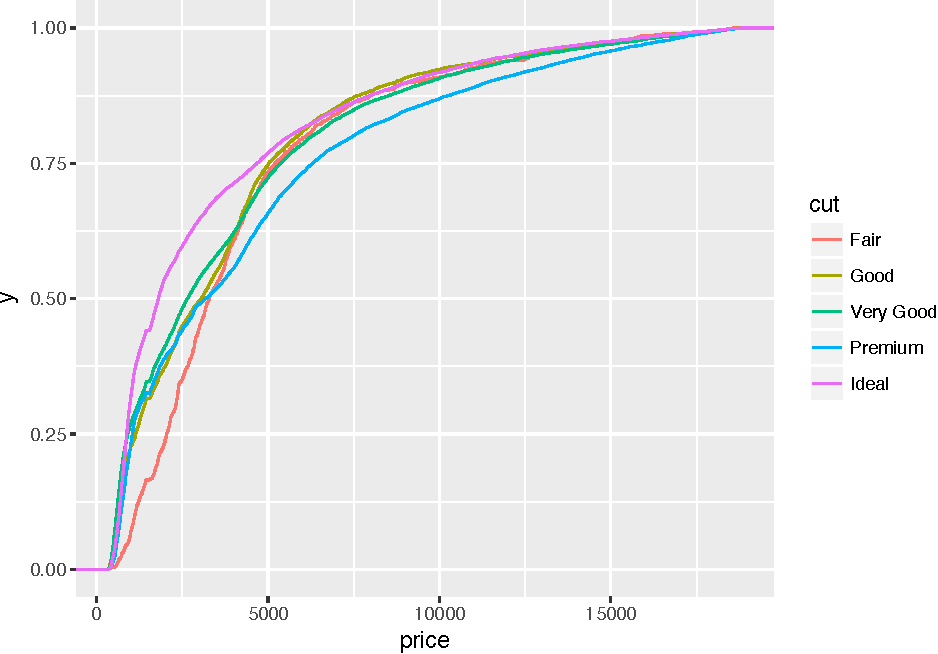
\includegraphics{visualizationwithggplot_files/figure-latex/unnamed-chunk-6-1.pdf}

\section{Distribution: 2-D distribution and overplotting
revisited}\label{distribution-2-d-distribution-and-overplotting-revisited}

\begin{Shaded}
\begin{Highlighting}[]
\KeywordTok{ggplot}\NormalTok{(diamonds, }\KeywordTok{aes}\NormalTok{(}\KeywordTok{log}\NormalTok{(carat), }\KeywordTok{log}\NormalTok{(price)))}\OperatorTok{+}
\StringTok{  }\KeywordTok{geom_point}\NormalTok{(}\DataTypeTok{alpha =}\NormalTok{ .}\DecValTok{01}\NormalTok{)}\OperatorTok{+}\StringTok{ }
\StringTok{  }\KeywordTok{theme_bw}\NormalTok{()}
\end{Highlighting}
\end{Shaded}

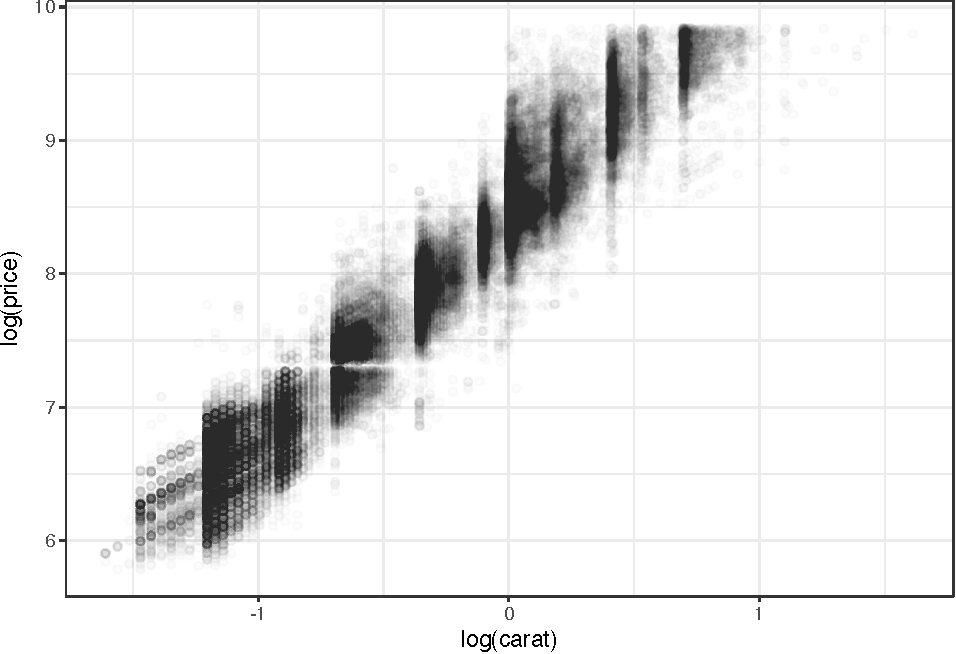
\includegraphics{visualizationwithggplot_files/figure-latex/unnamed-chunk-7-1.pdf}

\begin{Shaded}
\begin{Highlighting}[]
\KeywordTok{ggplot}\NormalTok{(diamonds, }\KeywordTok{aes}\NormalTok{(}\KeywordTok{log}\NormalTok{(carat), }\KeywordTok{log}\NormalTok{(price)))}\OperatorTok{+}
\StringTok{  }\KeywordTok{geom_point}\NormalTok{(}\DataTypeTok{size =}\NormalTok{ .}\DecValTok{5}\NormalTok{)}\OperatorTok{+}\StringTok{ }
\StringTok{  }\KeywordTok{geom_density2d}\NormalTok{(}\DataTypeTok{size=}\FloatTok{1.2}\NormalTok{)}\OperatorTok{+}
\StringTok{  }\KeywordTok{theme_bw}\NormalTok{()}
\end{Highlighting}
\end{Shaded}

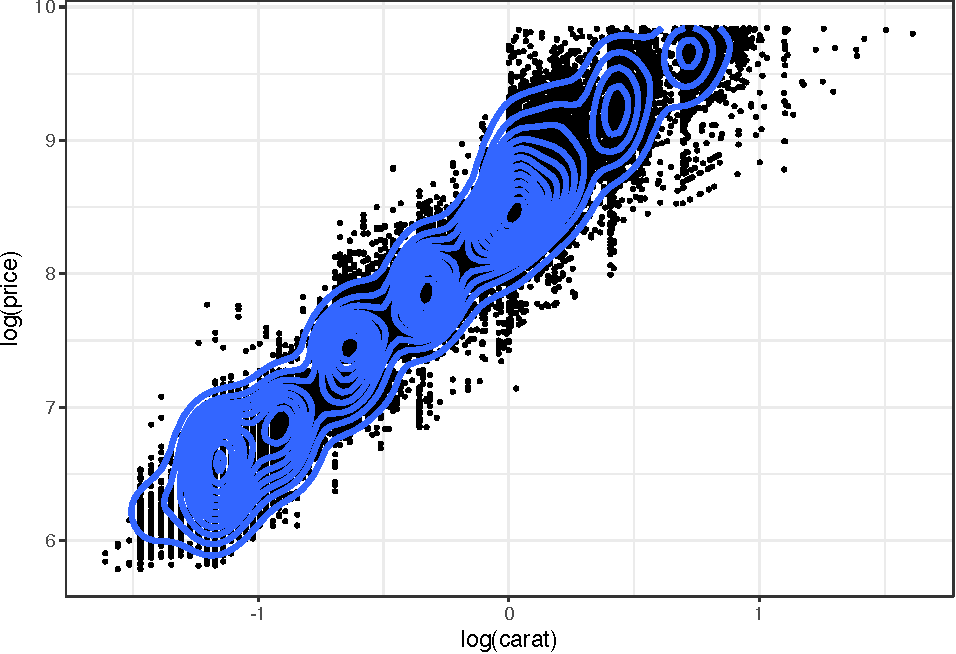
\includegraphics{visualizationwithggplot_files/figure-latex/unnamed-chunk-7-2.pdf}

\begin{Shaded}
\begin{Highlighting}[]
\KeywordTok{ggplot}\NormalTok{(diamonds, }\KeywordTok{aes}\NormalTok{(}\KeywordTok{log}\NormalTok{(carat), }\KeywordTok{log}\NormalTok{(price)))}\OperatorTok{+}
\StringTok{  }\KeywordTok{geom_point}\NormalTok{(}\DataTypeTok{size =}\NormalTok{ .}\DecValTok{5}\NormalTok{)}\OperatorTok{+}\StringTok{ }
\StringTok{  }\KeywordTok{geom_density2d}\NormalTok{(}\DataTypeTok{size=}\FloatTok{1.2}\NormalTok{)}\OperatorTok{+}
\StringTok{  }\KeywordTok{geom_hex}\NormalTok{(}\DataTypeTok{alpha =}\NormalTok{ .}\DecValTok{6}\NormalTok{) }\OperatorTok{+}
\StringTok{  }\KeywordTok{theme_bw}\NormalTok{()}
\end{Highlighting}
\end{Shaded}

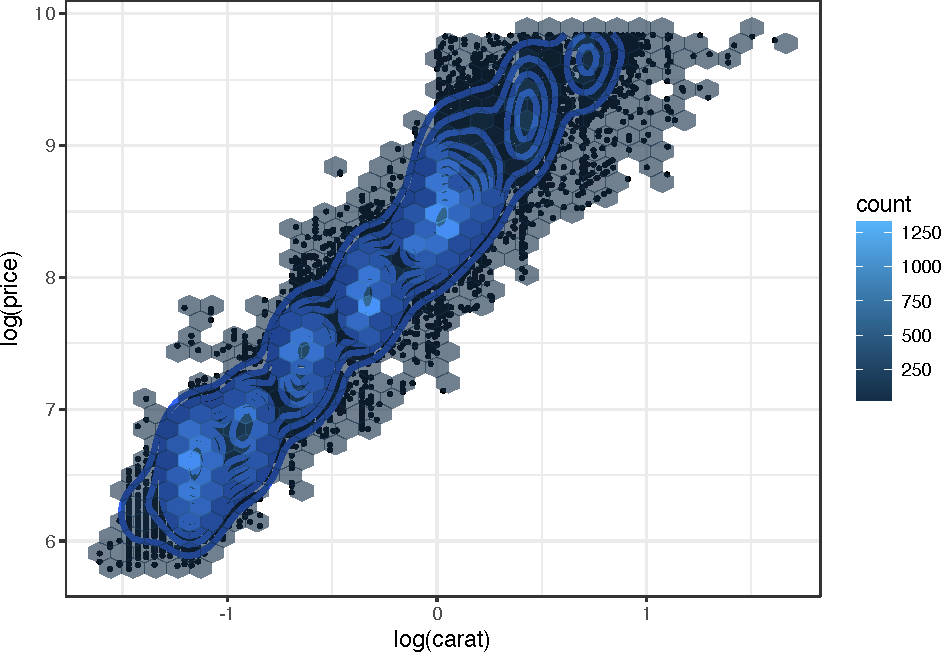
\includegraphics{visualizationwithggplot_files/figure-latex/unnamed-chunk-7-3.pdf}

\begin{Shaded}
\begin{Highlighting}[]
\KeywordTok{ggplot}\NormalTok{(diamonds, }\KeywordTok{aes}\NormalTok{(}\KeywordTok{log}\NormalTok{(carat), }\KeywordTok{log}\NormalTok{(price)))}\OperatorTok{+}
\StringTok{  }\CommentTok{#geom_point( )+}
\StringTok{  }\CommentTok{#geom_point(size = .5)+ }
\StringTok{  }\CommentTok{#geom_density2d(size=1.2)+}
\StringTok{  }\KeywordTok{geom_hex}\NormalTok{(}\DataTypeTok{bins =} \DecValTok{50}\NormalTok{) }\OperatorTok{+}
\StringTok{  }\KeywordTok{theme_bw}\NormalTok{()}
\end{Highlighting}
\end{Shaded}

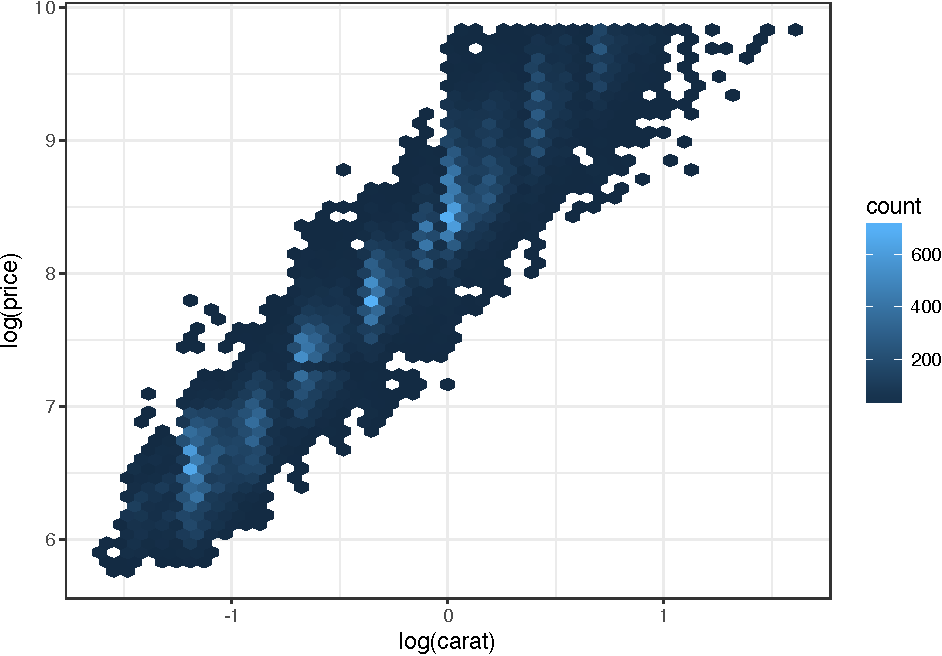
\includegraphics{visualizationwithggplot_files/figure-latex/unnamed-chunk-7-4.pdf}

\section{Histogram with density and median reference
line}\label{histogram-with-density-and-median-reference-line}

TODO change to diversity data gender across job types

\begin{Shaded}
\begin{Highlighting}[]
\NormalTok{diamonds.df =}\StringTok{ }\NormalTok{diamonds}

\NormalTok{sum.diamonds.df =}\StringTok{ }\NormalTok{diamonds.df }\OperatorTok\StringTok{ }\KeywordTok{group_by}\NormalTok{(cut) }\OperatorTok\StringTok{ }
\StringTok{  }\KeywordTok{summarise}\NormalTok{(}\DataTypeTok{q85 =} \KeywordTok{quantile}\NormalTok{(price, }\FloatTok{0.85}\NormalTok{))}

\KeywordTok{ggplot}\NormalTok{(}\DataTypeTok{data =}\NormalTok{ diamonds.df, }\KeywordTok{aes}\NormalTok{(price)) }\OperatorTok{+}\StringTok{ }
\StringTok{  }\KeywordTok{geom_histogram}\NormalTok{(}\KeywordTok{aes}\NormalTok{(}\DataTypeTok{y =}\NormalTok{ ..density..), }\DataTypeTok{bins =} \DecValTok{40}\NormalTok{) }\OperatorTok{+}\StringTok{ }
\StringTok{  }\KeywordTok{geom_density}\NormalTok{(}\DataTypeTok{colour =} \StringTok{"darkblue"}\NormalTok{) }\OperatorTok{+}
\StringTok{  }\KeywordTok{geom_vline}\NormalTok{(}\DataTypeTok{data =}\NormalTok{ sum.diamonds.df, }\KeywordTok{aes}\NormalTok{(}\DataTypeTok{xintercept =}\NormalTok{ q85)) }\OperatorTok{+}
\StringTok{  }\KeywordTok{facet_grid}\NormalTok{(cut }\OperatorTok{~}\StringTok{ }\NormalTok{.)}
\end{Highlighting}
\end{Shaded}

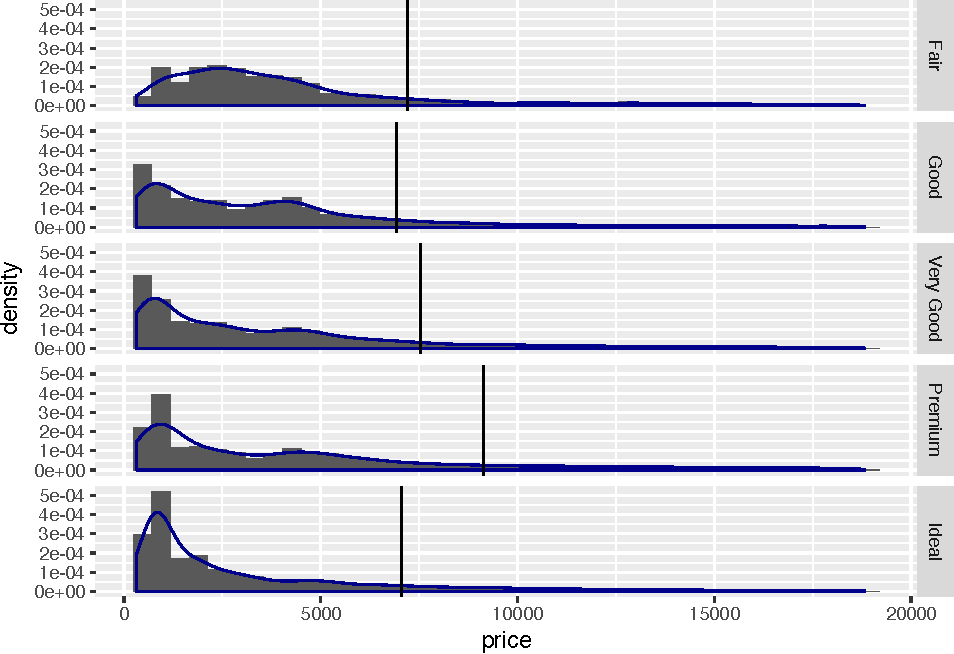
\includegraphics{visualizationwithggplot_files/figure-latex/unnamed-chunk-8-1.pdf}

\section{Ridge plot--An array of density
plots}\label{ridge-plotan-array-of-density-plots}

\url{https://cran.r-project.org/web/packages/ggridges/vignettes/gallery.html}

\begin{Shaded}
\begin{Highlighting}[]
\NormalTok{## Ridge plot}
\KeywordTok{library}\NormalTok{(ggridges)}
\end{Highlighting}
\end{Shaded}

\begin{verbatim}
## Warning: package 'ggridges' was built under R version
## 3.4.4
\end{verbatim}

\begin{Shaded}
\begin{Highlighting}[]
\KeywordTok{library}\NormalTok{(ggplot2movies)}

\NormalTok{movies }\OperatorTok\StringTok{ }\KeywordTok{filter}\NormalTok{(year}\OperatorTok{>}\DecValTok{1912}\NormalTok{, length}\OperatorTok{<}\DecValTok{250}\NormalTok{) }\OperatorTok\StringTok{ }
\KeywordTok{ggplot}\NormalTok{(}\KeywordTok{aes}\NormalTok{(}\DataTypeTok{x =}\NormalTok{ length, }\DataTypeTok{y =}\NormalTok{ year, }\DataTypeTok{group =}\NormalTok{ year)) }\OperatorTok{+}
\StringTok{  }\KeywordTok{geom_density_ridges}\NormalTok{(}\DataTypeTok{scale =} \DecValTok{10}\NormalTok{, }\DataTypeTok{size =} \FloatTok{0.25}\NormalTok{, }\DataTypeTok{rel_min_height =} \FloatTok{0.03}\NormalTok{, }\DataTypeTok{alpha=}\NormalTok{.}\DecValTok{75}\NormalTok{) }\OperatorTok{+}
\StringTok{  }\KeywordTok{scale_x_continuous}\NormalTok{(}\DataTypeTok{limits=}\KeywordTok{c}\NormalTok{(}\DecValTok{0}\NormalTok{, }\DecValTok{250}\NormalTok{), }\DataTypeTok{expand =} \KeywordTok{c}\NormalTok{(}\FloatTok{0.01}\NormalTok{, }\DecValTok{0}\NormalTok{)) }\OperatorTok{+}
\StringTok{  }\KeywordTok{scale_y_reverse}\NormalTok{(}\DataTypeTok{breaks=}\KeywordTok{c}\NormalTok{(}\DecValTok{2000}\NormalTok{, }\DecValTok{1980}\NormalTok{, }\DecValTok{1960}\NormalTok{, }\DecValTok{1940}\NormalTok{, }\DecValTok{1920}\NormalTok{, }\DecValTok{1900}\NormalTok{), }\DataTypeTok{expand =} \KeywordTok{c}\NormalTok{(}\FloatTok{0.01}\NormalTok{, }\DecValTok{0}\NormalTok{)) }\OperatorTok{+}
\StringTok{  }\KeywordTok{theme_ridges}\NormalTok{()}
\end{Highlighting}
\end{Shaded}

\begin{verbatim}
## Picking joint bandwidth of 6.89
\end{verbatim}

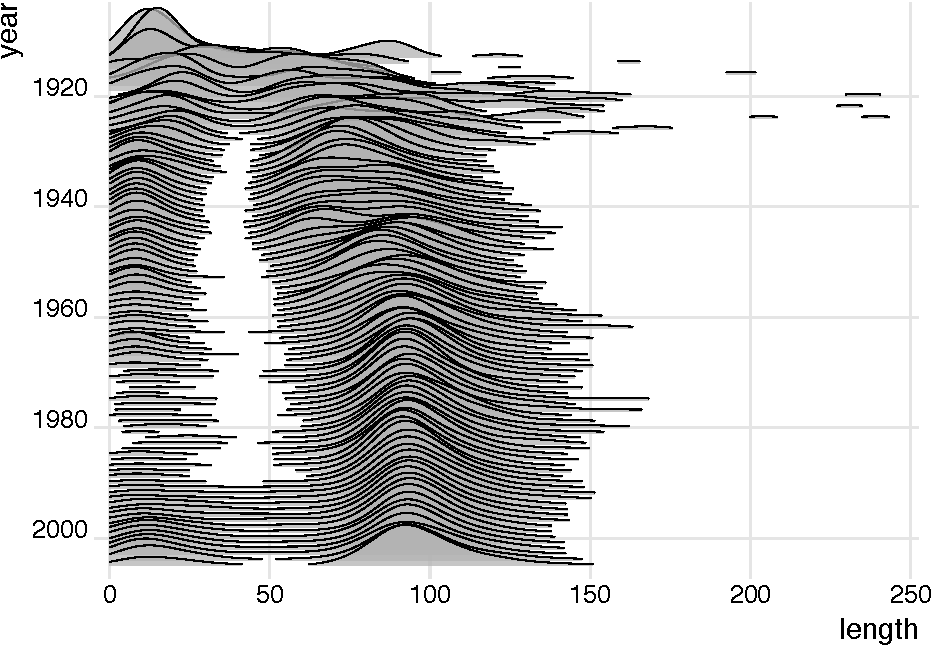
\includegraphics{visualizationwithggplot_files/figure-latex/unnamed-chunk-9-1.pdf}

\cleardoublepage 

\chapter{Comparison--barchart and boxplots}\label{Comparison}

\section{Graph considerations for communication: aggregation,
abstraction,
complexity}\label{graph-considerations-for-communication-aggregation-abstraction-complexity}

\subsection{Simple bar chart}\label{simple-bar-chart}

\begin{Shaded}
\begin{Highlighting}[]
\KeywordTok{library}\NormalTok{(tidyr)}
\KeywordTok{library}\NormalTok{(ggforce)}
\KeywordTok{library}\NormalTok{(ggthemes)}
\KeywordTok{library}\NormalTok{(ggstance)}

\NormalTok{mtcars.df =}\StringTok{ }\NormalTok{mtcars}
\NormalTok{mtcars.df =}\StringTok{ }\NormalTok{mtcars.df }\OperatorTok\StringTok{ }\KeywordTok{mutate}\NormalTok{(}\DataTypeTok{cyl =} \KeywordTok{as.factor}\NormalTok{(cyl))}

\NormalTok{s.mtcars.df =}\StringTok{ }\NormalTok{mtcars.df }\OperatorTok\StringTok{ }\KeywordTok{group_by}\NormalTok{(cyl) }\OperatorTok\StringTok{ }\KeywordTok{summarise}\NormalTok{(}\DataTypeTok{m.hp =} \KeywordTok{mean}\NormalTok{(hp), }\DataTypeTok{se.hp=} \KeywordTok{sd}\NormalTok{(hp)}\OperatorTok{/}\KeywordTok{n}\NormalTok{()}\OperatorTok{^}\NormalTok{.}\DecValTok{5}\NormalTok{)}


\KeywordTok{ggplot}\NormalTok{(}\DataTypeTok{data =}\NormalTok{ s.mtcars.df, }\KeywordTok{aes}\NormalTok{(}\DataTypeTok{x =}\NormalTok{ cyl, }\DataTypeTok{y =}\NormalTok{ m.hp)) }\OperatorTok{+}
\StringTok{  }\KeywordTok{geom_bar}\NormalTok{(}\DataTypeTok{stat=}\StringTok{"identity"}\NormalTok{)}
\end{Highlighting}
\end{Shaded}

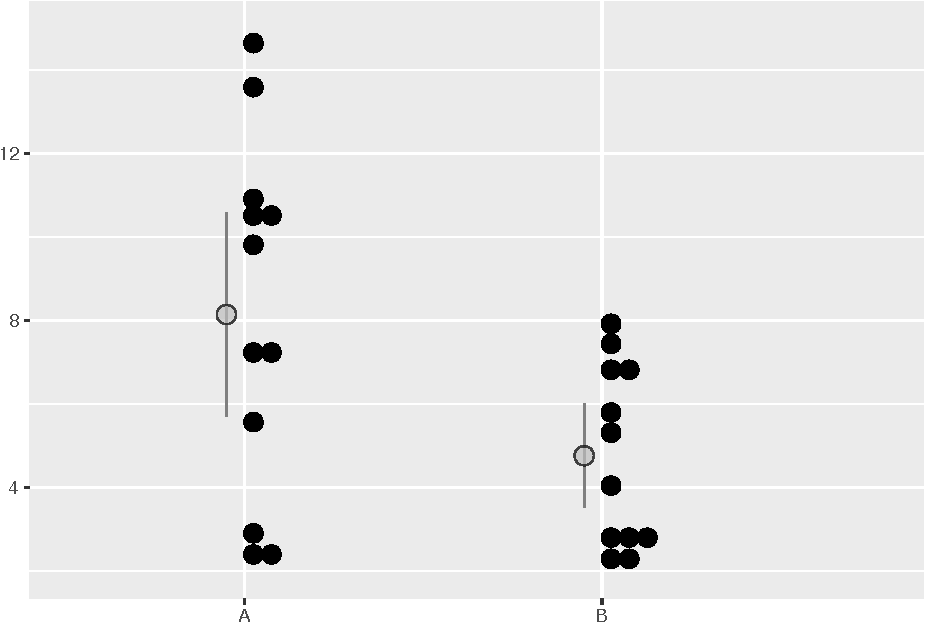
\includegraphics{visualizationwithggplot_files/figure-latex/unnamed-chunk-10-1.pdf}

\begin{Shaded}
\begin{Highlighting}[]
\KeywordTok{ggplot}\NormalTok{(}\DataTypeTok{data =}\NormalTok{ s.mtcars.df, }\KeywordTok{aes}\NormalTok{(}\DataTypeTok{x =}\NormalTok{ cyl, }\DataTypeTok{y =}\NormalTok{ m.hp)) }\OperatorTok{+}
\StringTok{  }\KeywordTok{geom_col}\NormalTok{()}
\end{Highlighting}
\end{Shaded}

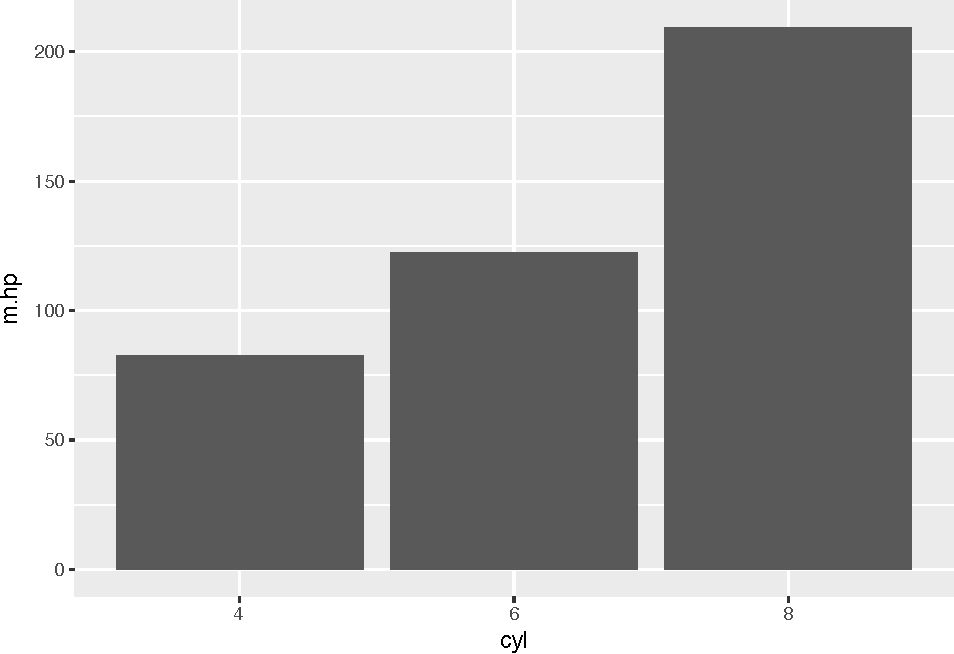
\includegraphics{visualizationwithggplot_files/figure-latex/unnamed-chunk-10-2.pdf}

\begin{Shaded}
\begin{Highlighting}[]
\NormalTok{## Change order of bars}
\NormalTok{cyl.order <-}\StringTok{ }\KeywordTok{c}\NormalTok{(}\StringTok{"8"}\NormalTok{, }\StringTok{"6"}\NormalTok{, }\StringTok{"4"}\NormalTok{)}
\KeywordTok{ggplot}\NormalTok{(}\DataTypeTok{data =}\NormalTok{ s.mtcars.df, }\KeywordTok{aes}\NormalTok{(}\DataTypeTok{x =}\NormalTok{ cyl, }\DataTypeTok{y =}\NormalTok{ m.hp)) }\OperatorTok{+}
\StringTok{  }\KeywordTok{geom_col}\NormalTok{() }\OperatorTok{+}
\StringTok{  }\KeywordTok{scale_x_discrete}\NormalTok{(}\DataTypeTok{limits =}\NormalTok{ cyl.order)}
\end{Highlighting}
\end{Shaded}

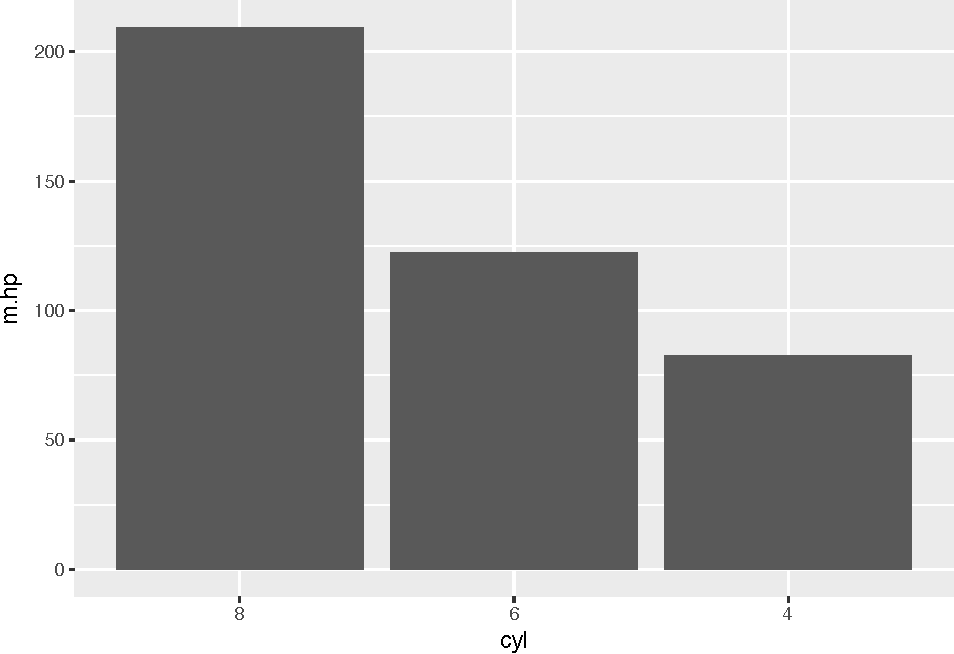
\includegraphics{visualizationwithggplot_files/figure-latex/unnamed-chunk-10-3.pdf}

\subsection{Bar chart with error bars}\label{bar-chart-with-error-bars}

\begin{Shaded}
\begin{Highlighting}[]
\KeywordTok{ggplot}\NormalTok{(}\DataTypeTok{data =}\NormalTok{ s.mtcars.df, }\KeywordTok{aes}\NormalTok{(}\DataTypeTok{x =}\NormalTok{ cyl, }\DataTypeTok{y =}\NormalTok{ m.hp)) }\OperatorTok{+}
\StringTok{  }\KeywordTok{geom_bar}\NormalTok{(}\DataTypeTok{stat=}\StringTok{"identity"}\NormalTok{)}\OperatorTok{+}
\StringTok{  }\KeywordTok{geom_linerange}\NormalTok{(}\KeywordTok{aes}\NormalTok{(}\DataTypeTok{ymin=}\NormalTok{m.hp}\OperatorTok{-}\DecValTok{2}\OperatorTok{*}\NormalTok{se.hp, }\DataTypeTok{ymax=}\NormalTok{m.hp}\OperatorTok{+}\DecValTok{2}\OperatorTok{*}\NormalTok{se.hp))}
\end{Highlighting}
\end{Shaded}

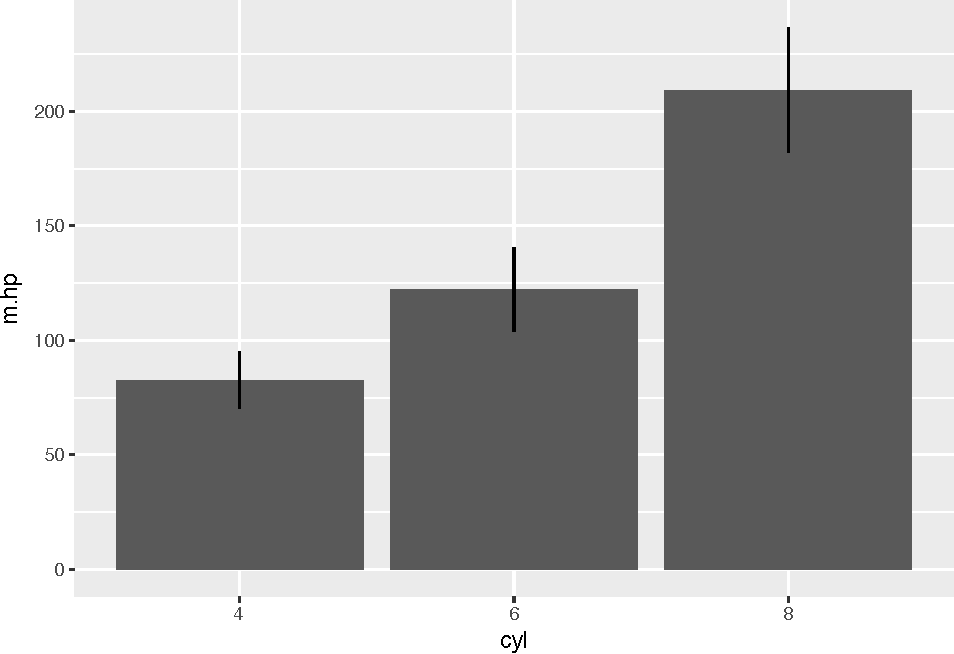
\includegraphics{visualizationwithggplot_files/figure-latex/unnamed-chunk-11-1.pdf}

\begin{Shaded}
\begin{Highlighting}[]
\KeywordTok{ggplot}\NormalTok{(}\DataTypeTok{data =}\NormalTok{ s.mtcars.df, }\KeywordTok{aes}\NormalTok{(}\DataTypeTok{x =}\NormalTok{ cyl, }\DataTypeTok{y =}\NormalTok{ m.hp)) }\OperatorTok{+}
\StringTok{  }\KeywordTok{geom_bar}\NormalTok{(}\DataTypeTok{stat=}\StringTok{"identity"}\NormalTok{)}\OperatorTok{+}
\StringTok{  }\KeywordTok{geom_linerange}\NormalTok{(}\KeywordTok{aes}\NormalTok{(}\DataTypeTok{ymin=}\NormalTok{m.hp}\OperatorTok{-}\DecValTok{2}\OperatorTok{*}\NormalTok{se.hp, }\DataTypeTok{ymax=}\NormalTok{m.hp}\OperatorTok{+}\DecValTok{2}\OperatorTok{*}\NormalTok{se.hp))}\OperatorTok{+}
\StringTok{  }\KeywordTok{geom_point}\NormalTok{(}\DataTypeTok{data =}\NormalTok{ mtcars.df, }\KeywordTok{aes}\NormalTok{(cyl, hp), }\DataTypeTok{position =} \KeywordTok{position_jitter}\NormalTok{(}\DataTypeTok{width =}\NormalTok{ .}\DecValTok{2}\NormalTok{, }\DataTypeTok{height =} \DecValTok{0}\NormalTok{))}
\end{Highlighting}
\end{Shaded}

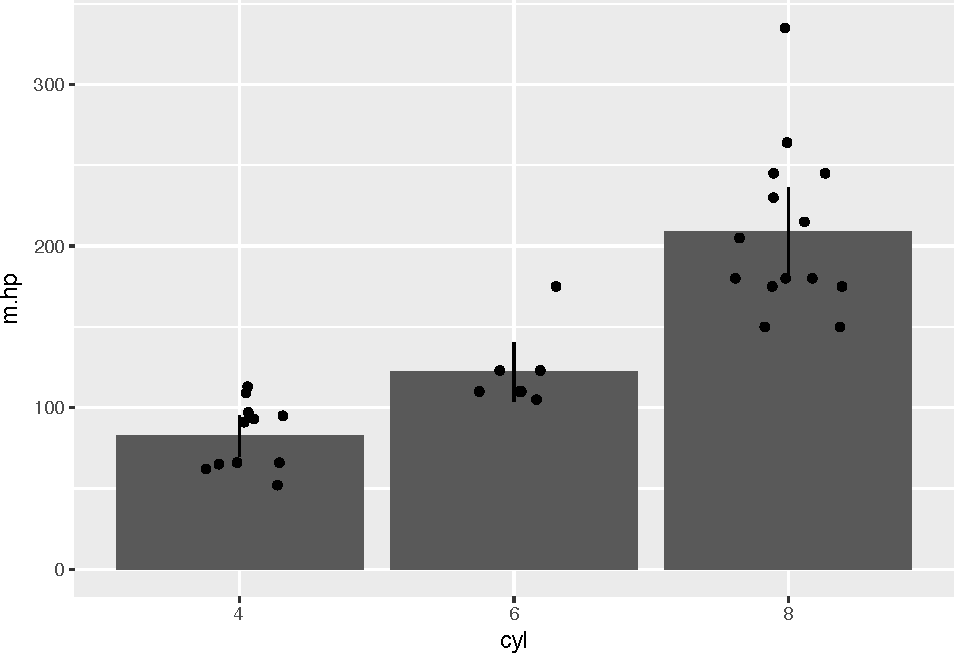
\includegraphics{visualizationwithggplot_files/figure-latex/unnamed-chunk-11-2.pdf}

\subsection{dotplot and offset range
plot}\label{dotplot-and-offset-range-plot}

\begin{Shaded}
\begin{Highlighting}[]
\NormalTok{## Set seed and create data}
\KeywordTok{set.seed}\NormalTok{(}\DecValTok{999}\NormalTok{)}
\NormalTok{df =}\StringTok{ }\KeywordTok{data_frame}\NormalTok{(}\DataTypeTok{A =} \KeywordTok{runif}\NormalTok{(}\DecValTok{12}\NormalTok{,}\DecValTok{1}\NormalTok{,}\DecValTok{17}\NormalTok{), }\DataTypeTok{B =} \KeywordTok{runif}\NormalTok{(}\DecValTok{12}\NormalTok{, }\DecValTok{2}\NormalTok{, }\DecValTok{8}\NormalTok{))}


\NormalTok{l.df =}\StringTok{ }\KeywordTok{gather}\NormalTok{(df, condition, value)}
\NormalTok{l.df}\OperatorTok{$}\NormalTok{condition =}\StringTok{ }\KeywordTok{as.factor}\NormalTok{(l.df}\OperatorTok{$}\NormalTok{condition)}
\NormalTok{m.l.df =}\StringTok{ }\NormalTok{l.df }\OperatorTok\StringTok{ }\KeywordTok{group_by}\NormalTok{(condition) }\OperatorTok\StringTok{ }\KeywordTok{summarise}\NormalTok{(}\DataTypeTok{m.value =} \KeywordTok{mean}\NormalTok{(value, }\DataTypeTok{na.rm=}\OtherTok{TRUE}\NormalTok{), }
      \DataTypeTok{n=} \KeywordTok{sum}\NormalTok{(}\OperatorTok{!}\KeywordTok{is.na}\NormalTok{(value)), }\DataTypeTok{sd=}\KeywordTok{sd}\NormalTok{(value, }\DataTypeTok{na.rm=}\OtherTok{TRUE}\NormalTok{), }\DataTypeTok{sde=}\KeywordTok{sd}\NormalTok{(value, }\DataTypeTok{na.rm=}\OtherTok{TRUE}\NormalTok{)}\OperatorTok{/}\NormalTok{n}\OperatorTok{^}\NormalTok{.}\DecValTok{5}\NormalTok{,}
       \DataTypeTok{ci=} \DecValTok{2}\OperatorTok{*}\NormalTok{sde)}
\NormalTok{m.l.df}\OperatorTok{$}\NormalTok{n.condition =}\StringTok{ }\KeywordTok{as.numeric}\NormalTok{(m.l.df}\OperatorTok{$}\NormalTok{condition)}\OperatorTok{-}\NormalTok{.}\DecValTok{05} 


\NormalTok{## Plot with offset for mean and error bar}
\KeywordTok{ggplot}\NormalTok{()}\OperatorTok{+}
\StringTok{  }\KeywordTok{geom_dotplot}\NormalTok{(}\DataTypeTok{data =} \KeywordTok{filter}\NormalTok{(l.df, condition}\OperatorTok{==}\StringTok{"A"}\OperatorTok{|}\NormalTok{condition}\OperatorTok{==}\StringTok{"B"}\NormalTok{),}
               \KeywordTok{aes}\NormalTok{(condition, value), }\DataTypeTok{binaxis =} \StringTok{"y"}\NormalTok{, }\DataTypeTok{stackdir =} \StringTok{"up"}\NormalTok{)}\OperatorTok{+}
\StringTok{  }\KeywordTok{geom_linerange}\NormalTok{(}\DataTypeTok{data =} \KeywordTok{filter}\NormalTok{(m.l.df, condition}\OperatorTok{==}\StringTok{"A"}\OperatorTok{|}\NormalTok{condition}\OperatorTok{==}\StringTok{"B"}\NormalTok{), }
                 \KeywordTok{aes}\NormalTok{(n.condition, }\DataTypeTok{ymin=}\NormalTok{m.value}\OperatorTok{-}\NormalTok{ci, }\DataTypeTok{ymax=}\NormalTok{m.value}\OperatorTok{+}\NormalTok{ci), }\DataTypeTok{color=}\StringTok{"grey50"}\NormalTok{) }\OperatorTok{+}
\StringTok{  }\KeywordTok{geom_point}\NormalTok{(}\DataTypeTok{data =} \KeywordTok{filter}\NormalTok{(m.l.df, condition}\OperatorTok{==}\StringTok{"A"}\OperatorTok{|}\NormalTok{condition}\OperatorTok{==}\StringTok{"B"}\NormalTok{), }
             \KeywordTok{aes}\NormalTok{(n.condition, }\DataTypeTok{y=}\NormalTok{ m.value), }\DataTypeTok{shape =} \DecValTok{21}\NormalTok{, }\DataTypeTok{size =} \DecValTok{4}\NormalTok{, }\DataTypeTok{fill=}\StringTok{"grey"}\NormalTok{, }\DataTypeTok{alpha=}\NormalTok{.}\DecValTok{7}\NormalTok{) }\OperatorTok{+}
\StringTok{  }\KeywordTok{labs}\NormalTok{(}\DataTypeTok{x=}\StringTok{""}\NormalTok{, }\DataTypeTok{y=}\StringTok{""}\NormalTok{) }\OperatorTok{+}
\StringTok{  }\KeywordTok{ylim}\NormalTok{(}\DecValTok{2}\NormalTok{, }\DecValTok{15}\NormalTok{)}
\end{Highlighting}
\end{Shaded}

\begin{verbatim}
## `stat_bindot()` using `bins = 30`. Pick better value with `binwidth`.
\end{verbatim}

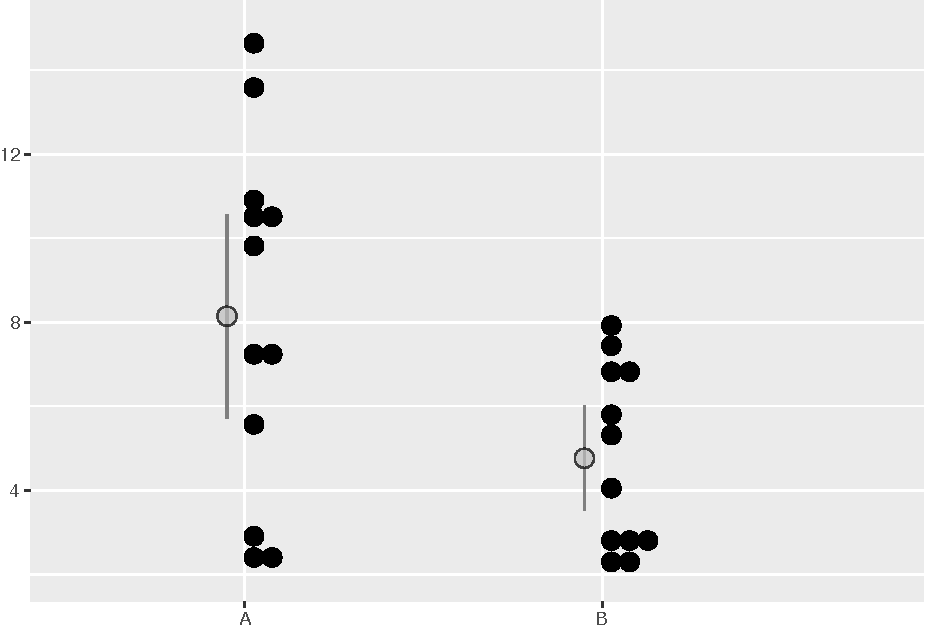
\includegraphics{visualizationwithggplot_files/figure-latex/unnamed-chunk-12-1.pdf}

\subsection{Statistical significance in
context}\label{statistical-significance-in-context}

\begin{Shaded}
\begin{Highlighting}[]
\KeywordTok{ggplot}\NormalTok{(}\DataTypeTok{data =}\NormalTok{ mtcars.df, }\KeywordTok{aes}\NormalTok{(}\DataTypeTok{x =} \KeywordTok{as.factor}\NormalTok{(cyl), }\DataTypeTok{y =}\NormalTok{ hp)) }\OperatorTok{+}\StringTok{ }
\StringTok{  }\KeywordTok{geom_boxplot}\NormalTok{(}\DataTypeTok{colour =} \StringTok{"darkgrey"}\NormalTok{) }\OperatorTok{+}\StringTok{ }
\StringTok{  }\KeywordTok{geom_point}\NormalTok{(}\DataTypeTok{stat=}\StringTok{"summary"}\NormalTok{, }\DataTypeTok{fun.y =} \StringTok{"mean"}\NormalTok{, }\DataTypeTok{size =} \DecValTok{6}\NormalTok{, }\DataTypeTok{shape =} \DecValTok{1}\NormalTok{) }\OperatorTok{+}
\StringTok{  }\KeywordTok{geom_pointrange}\NormalTok{(}\DataTypeTok{stat=}\StringTok{"summary"}\NormalTok{, }\DataTypeTok{fun.data =} \StringTok{"mean_cl_boot"}\NormalTok{) }\OperatorTok{+}
\StringTok{  }\KeywordTok{geom_dotplot}\NormalTok{(}\DataTypeTok{binaxis =} \StringTok{"y"}\NormalTok{, }\DataTypeTok{stackdir =} \StringTok{"center"}\NormalTok{, }\DataTypeTok{binwidth =} \DecValTok{1}\NormalTok{, }
               \DataTypeTok{dotsize =} \DecValTok{6}\NormalTok{,}\DataTypeTok{alpha =}\NormalTok{ .}\DecValTok{3}\NormalTok{, }\DataTypeTok{color =} \StringTok{"black"}\NormalTok{, }\DataTypeTok{fill =} \StringTok{"red"}\NormalTok{) }\OperatorTok{+}
\StringTok{  }\KeywordTok{geom_hline}\NormalTok{(}\KeywordTok{aes}\NormalTok{(}\DataTypeTok{yintercept =} \KeywordTok{mean}\NormalTok{(hp)), }\DataTypeTok{size =} \FloatTok{1.2}\NormalTok{) }
\end{Highlighting}
\end{Shaded}

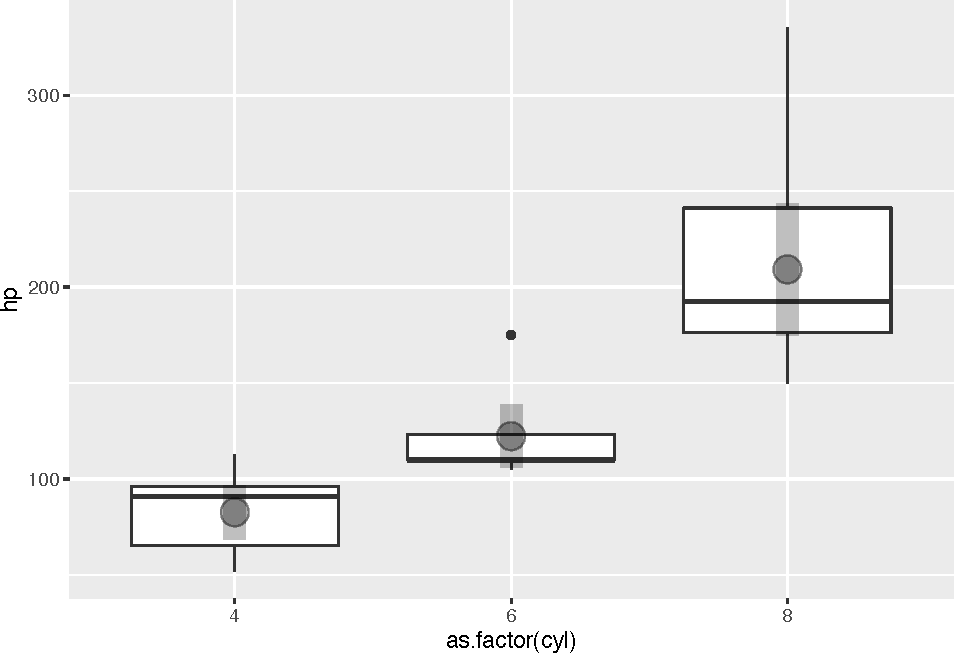
\includegraphics{visualizationwithggplot_files/figure-latex/unnamed-chunk-13-1.pdf}

\section{Comparing distributions, box, violyn, and sina
plot}\label{comparing-distributions-box-violyn-and-sina-plot}

\begin{Shaded}
\begin{Highlighting}[]
\KeywordTok{library}\NormalTok{(tidyr)}

\KeywordTok{ggplot}\NormalTok{(}\DataTypeTok{data =}\NormalTok{ s.mtcars.df, }\KeywordTok{aes}\NormalTok{(}\DataTypeTok{x =}\NormalTok{ cyl, }\DataTypeTok{y =}\NormalTok{ m.hp)) }\OperatorTok{+}
\StringTok{  }\KeywordTok{geom_col}\NormalTok{()}\OperatorTok{+}
\StringTok{  }\KeywordTok{geom_linerange}\NormalTok{(}\KeywordTok{aes}\NormalTok{(}\DataTypeTok{ymin=}\NormalTok{m.hp}\OperatorTok{-}\DecValTok{2}\OperatorTok{*}\NormalTok{se.hp, }\DataTypeTok{ymax=}\NormalTok{m.hp}\OperatorTok{+}\DecValTok{2}\OperatorTok{*}\NormalTok{se.hp))}
\end{Highlighting}
\end{Shaded}

\includegraphics{visualizationwithggplot_files/figure-latex/unnamed-chunk-14-1.pdf}

\begin{Shaded}
\begin{Highlighting}[]
\KeywordTok{ggplot}\NormalTok{(}\DataTypeTok{data =}\NormalTok{ s.mtcars.df, }\KeywordTok{aes}\NormalTok{(}\DataTypeTok{x =}\NormalTok{ cyl, }\DataTypeTok{y =}\NormalTok{ m.hp)) }\OperatorTok{+}
\StringTok{  }\KeywordTok{geom_col}\NormalTok{()}\OperatorTok{+}
\StringTok{  }\KeywordTok{geom_linerange}\NormalTok{(}\KeywordTok{aes}\NormalTok{(}\DataTypeTok{ymin=}\NormalTok{m.hp}\OperatorTok{-}\DecValTok{2}\OperatorTok{*}\NormalTok{se.hp, }\DataTypeTok{ymax=}\NormalTok{m.hp}\OperatorTok{+}\DecValTok{2}\OperatorTok{*}\NormalTok{se.hp))}\OperatorTok{+}
\StringTok{  }\KeywordTok{geom_point}\NormalTok{(}\DataTypeTok{data =}\NormalTok{ mtcars.df, }\KeywordTok{aes}\NormalTok{(cyl, hp), }\DataTypeTok{position =} \KeywordTok{position_jitter}\NormalTok{(}\DataTypeTok{width =}\NormalTok{ .}\DecValTok{2}\NormalTok{, }\DataTypeTok{height =} \DecValTok{0}\NormalTok{))}
\end{Highlighting}
\end{Shaded}

\includegraphics{visualizationwithggplot_files/figure-latex/unnamed-chunk-14-2.pdf}

\begin{Shaded}
\begin{Highlighting}[]
\KeywordTok{ggplot}\NormalTok{(}\DataTypeTok{data =}\NormalTok{ s.mtcars.df, }\KeywordTok{aes}\NormalTok{(}\DataTypeTok{x =}\NormalTok{ cyl, }\DataTypeTok{y =}\NormalTok{ m.hp)) }\OperatorTok{+}
\StringTok{  }\KeywordTok{geom_point}\NormalTok{(}\DataTypeTok{stat=}\StringTok{"identity"}\NormalTok{, }\DataTypeTok{size =} \DecValTok{3}\NormalTok{)}\OperatorTok{+}
\StringTok{  }\KeywordTok{geom_linerange}\NormalTok{(}\KeywordTok{aes}\NormalTok{(}\DataTypeTok{ymin=}\NormalTok{m.hp}\OperatorTok{-}\DecValTok{2}\OperatorTok{*}\NormalTok{se.hp, }\DataTypeTok{ymax=}\NormalTok{m.hp}\OperatorTok{+}\DecValTok{2}\OperatorTok{*}\NormalTok{se.hp))}\OperatorTok{+}
\StringTok{  }\KeywordTok{geom_point}\NormalTok{(}\DataTypeTok{data =}\NormalTok{ mtcars.df, }\KeywordTok{aes}\NormalTok{(cyl, hp), }\DataTypeTok{position =} \KeywordTok{position_jitter}\NormalTok{(}\DataTypeTok{width =}\NormalTok{ .}\DecValTok{2}\NormalTok{, }\DataTypeTok{height =} \DecValTok{0}\NormalTok{))}
\end{Highlighting}
\end{Shaded}

\includegraphics{visualizationwithggplot_files/figure-latex/unnamed-chunk-14-3.pdf}

\begin{Shaded}
\begin{Highlighting}[]
\NormalTok{## Sina plot}
\KeywordTok{ggplot}\NormalTok{(mpg, }\KeywordTok{aes}\NormalTok{(}\KeywordTok{as.factor}\NormalTok{(cyl), hwy))}\OperatorTok{+}
\StringTok{ }\KeywordTok{geom_sina}\NormalTok{(}\KeywordTok{aes}\NormalTok{(}\DataTypeTok{color =} \KeywordTok{as.factor}\NormalTok{(cyl)),}\DataTypeTok{size =} \DecValTok{1}\NormalTok{, }\DataTypeTok{alpha =}\NormalTok{.}\DecValTok{5}\NormalTok{) }\OperatorTok{+}
\StringTok{ }\KeywordTok{geom_tufteboxplot}\NormalTok{()}\OperatorTok{+}
\StringTok{  }\KeywordTok{labs}\NormalTok{(}\DataTypeTok{title =} \StringTok{"ggforce: sina plot with Tufte boxplot"}\NormalTok{)}
\end{Highlighting}
\end{Shaded}

\includegraphics{visualizationwithggplot_files/figure-latex/unnamed-chunk-14-4.pdf}

\begin{Shaded}
\begin{Highlighting}[]
\CommentTok{# ggplot(s.mtcars.df, aes(m.hp, m.mpg, colour =as.factor(cyl)))+}
\CommentTok{# geom_pointrangeh(aes(xmin= m.hp-se.hp, xmax = m.hp+se.hp))+}
\CommentTok{#   geom_pointrange(aes(ymin= m.mpg-se.mpg, ymax = m.mpg+se.mpg))+}
\CommentTok{#   labs(title = "ggstance: horizontal point range")}


\KeywordTok{ggplot}\NormalTok{(}\DataTypeTok{data =}\NormalTok{ s.mtcars.df, }\KeywordTok{aes}\NormalTok{(}\DataTypeTok{x =}\NormalTok{ cyl, }\DataTypeTok{y =}\NormalTok{ m.hp)) }\OperatorTok{+}
\StringTok{  }\KeywordTok{geom_violin}\NormalTok{(}\DataTypeTok{data=}\NormalTok{ mtcars.df, }\KeywordTok{aes}\NormalTok{(cyl, hp))}\OperatorTok{+}
\StringTok{  }\KeywordTok{geom_point}\NormalTok{(}\DataTypeTok{stat=}\StringTok{"identity"}\NormalTok{, }\DataTypeTok{size =} \DecValTok{3}\NormalTok{)}\OperatorTok{+}
\StringTok{  }\KeywordTok{geom_linerange}\NormalTok{(}\KeywordTok{aes}\NormalTok{(}\DataTypeTok{ymin=}\NormalTok{m.hp}\OperatorTok{-}\DecValTok{2}\OperatorTok{*}\NormalTok{se.hp, }\DataTypeTok{ymax=}\NormalTok{m.hp}\OperatorTok{+}\DecValTok{2}\OperatorTok{*}\NormalTok{se.hp))}\OperatorTok{+}
\StringTok{  }\KeywordTok{geom_point}\NormalTok{(}\DataTypeTok{data =}\NormalTok{ mtcars.df, }\KeywordTok{aes}\NormalTok{(cyl, hp), }
             \DataTypeTok{position =} \KeywordTok{position_jitter}\NormalTok{(}\DataTypeTok{width =}\NormalTok{ .}\DecValTok{2}\NormalTok{, }\DataTypeTok{height =} \DecValTok{0}\NormalTok{), }\DataTypeTok{alpha =}\NormalTok{.}\DecValTok{6}\NormalTok{)}
\end{Highlighting}
\end{Shaded}

\includegraphics{visualizationwithggplot_files/figure-latex/unnamed-chunk-14-5.pdf}

\subsection{Compare empirical and theoretical
distribution}\label{compare-empirical-and-theoretical-distribution}

\begin{Shaded}
\begin{Highlighting}[]
\NormalTok{sum.mtcars.df =}\StringTok{ }\NormalTok{mtcars.df}\OperatorTok\StringTok{ }\KeywordTok{group_by}\NormalTok{(cyl) }\OperatorTok\StringTok{ }
\StringTok{    }\KeywordTok{summarise}\NormalTok{(}\DataTypeTok{m.hp =} \KeywordTok{mean}\NormalTok{(hp), }\DataTypeTok{sd.hp =} \KeywordTok{sd}\NormalTok{(hp))}

\KeywordTok{ggplot}\NormalTok{(mtcars.df) }\OperatorTok{+}
\StringTok{  }\KeywordTok{geom_boxplot}\NormalTok{(}\KeywordTok{aes}\NormalTok{(}\KeywordTok{as.factor}\NormalTok{(cyl), hp)) }\OperatorTok{+}
\StringTok{  }\KeywordTok{geom_linerange}\NormalTok{(}\DataTypeTok{data =}\NormalTok{ sum.mtcars.df,}
        \KeywordTok{aes}\NormalTok{(}\DataTypeTok{x =} \KeywordTok{as.factor}\NormalTok{(cyl), }
        \DataTypeTok{ymin =}\NormalTok{ m.hp }\OperatorTok{+}\StringTok{ }\KeywordTok{qnorm}\NormalTok{(.}\DecValTok{25}\NormalTok{)}\OperatorTok{*}\NormalTok{sd.hp, }\DataTypeTok{ymax =}\NormalTok{ m.hp }\OperatorTok{+}\StringTok{ }\KeywordTok{qnorm}\NormalTok{(.}\DecValTok{75}\NormalTok{)}\OperatorTok{*}\NormalTok{sd.hp),}
                 \DataTypeTok{size =} \DecValTok{5}\NormalTok{, }\DataTypeTok{alpha =}\NormalTok{ .}\DecValTok{25}\NormalTok{) }\OperatorTok{+}
\StringTok{  }\KeywordTok{geom_point}\NormalTok{(}\DataTypeTok{data =}\NormalTok{ sum.mtcars.df,}
         \KeywordTok{aes}\NormalTok{(}\KeywordTok{as.factor}\NormalTok{(cyl), }\DataTypeTok{y=}\NormalTok{ m.hp),}\DataTypeTok{size =} \DecValTok{6}\NormalTok{, }\DataTypeTok{alpha =}\NormalTok{ .}\DecValTok{33}\NormalTok{)}
\end{Highlighting}
\end{Shaded}

\includegraphics{visualizationwithggplot_files/figure-latex/unnamed-chunk-15-1.pdf}

\subsection{Tufte-inspired minimal bar
chart}\label{tufte-inspired-minimal-bar-chart}

\url{http://motioninsocial.com/tufte/}

\begin{Shaded}
\begin{Highlighting}[]
\CommentTok{#TODO replace with better dataset with for more columns}
\KeywordTok{library}\NormalTok{(ggthemes)}
\KeywordTok{ggplot}\NormalTok{(mtcars.df, }\KeywordTok{aes}\NormalTok{(}\DataTypeTok{x=}\KeywordTok{as.factor}\NormalTok{(cyl))) }\OperatorTok{+}\StringTok{ }
\StringTok{  }\KeywordTok{geom_bar}\NormalTok{(}\DataTypeTok{width=}\FloatTok{0.25}\NormalTok{, }\DataTypeTok{fill=}\StringTok{"gray"}\NormalTok{) }\OperatorTok{+}\StringTok{  }
\StringTok{  }\KeywordTok{scale_y_continuous}\NormalTok{(}\DataTypeTok{breaks=}\KeywordTok{seq}\NormalTok{(}\DecValTok{2}\NormalTok{, }\DecValTok{12}\NormalTok{, }\DecValTok{2}\NormalTok{)) }\OperatorTok{+}\StringTok{ }
\StringTok{  }\KeywordTok{geom_hline}\NormalTok{(}\DataTypeTok{yintercept=}\KeywordTok{seq}\NormalTok{(}\DecValTok{2}\NormalTok{, }\DecValTok{12}\NormalTok{, }\DecValTok{2}\NormalTok{), }\DataTypeTok{colour=}\StringTok{"white"}\NormalTok{, }\DataTypeTok{lwd=}\DecValTok{1}\NormalTok{) }\OperatorTok{+}
\StringTok{  }\KeywordTok{theme_tufte}\NormalTok{(}\DataTypeTok{base_size=}\DecValTok{12}\NormalTok{, }\DataTypeTok{ticks=}\NormalTok{F, }\DataTypeTok{base_family =} \StringTok{"Arial"}\NormalTok{) }
\end{Highlighting}
\end{Shaded}

\includegraphics{visualizationwithggplot_files/figure-latex/unnamed-chunk-16-1.pdf}

\section{Comparing across many
variables}\label{comparing-across-many-variables}

\subsection{Dot plots and reordering}\label{dot-plots-and-reordering}

Comparing many mean values

\begin{Shaded}
\begin{Highlighting}[]
\CommentTok{#TODO Change to mean sd catepilar plot}
\NormalTok{mtcars.df =}\StringTok{ }\NormalTok{mtcars}
\NormalTok{mtcars.df}\OperatorTok{$}\NormalTok{name =}\StringTok{ }\KeywordTok{rownames}\NormalTok{(mtcars.df)}
\KeywordTok{ggplot}\NormalTok{(}\DataTypeTok{data =}\NormalTok{ mtcars.df, }\KeywordTok{aes}\NormalTok{(}\KeywordTok{reorder}\NormalTok{(name, hp), }\DataTypeTok{y =}\NormalTok{ hp, }\DataTypeTok{colour =} \KeywordTok{as.factor}\NormalTok{(cyl))) }\OperatorTok{+}
\StringTok{  }\KeywordTok{geom_point}\NormalTok{(}\DataTypeTok{size =} \DecValTok{2}\NormalTok{) }\OperatorTok{+}
\StringTok{  }\KeywordTok{geom_hline}\NormalTok{(}\KeywordTok{aes}\NormalTok{(}\DataTypeTok{yintercept =} \KeywordTok{mean}\NormalTok{(hp)), }\DataTypeTok{colour =} \StringTok{"darkgrey"}\NormalTok{) }\OperatorTok{+}
\StringTok{  }\KeywordTok{geom_linerange}\NormalTok{(}\KeywordTok{aes}\NormalTok{(}\DataTypeTok{ymin=} \OperatorTok{-}\OtherTok{Inf}\NormalTok{, }\DataTypeTok{ymax=}\NormalTok{ hp), }\DataTypeTok{alpha =}\NormalTok{.}\DecValTok{5}\NormalTok{) }\OperatorTok{+}
\StringTok{  }\KeywordTok{coord_flip}\NormalTok{() }\OperatorTok{+}
\StringTok{  }\KeywordTok{labs}\NormalTok{(}\DataTypeTok{x =} \StringTok{"Cylinders"}\NormalTok{, }\DataTypeTok{y =} \StringTok{"Power (hp)"}\NormalTok{) }\OperatorTok{+}
\StringTok{  }\KeywordTok{scale_colour_brewer}\NormalTok{(}\DataTypeTok{name =} \StringTok{"Number of }\CharTok{\textbackslash{}n}\StringTok{Cylinders"}\NormalTok{, }\DataTypeTok{palette=}\StringTok{"Dark2"}\NormalTok{) }\OperatorTok{+}\StringTok{ }\CommentTok{# http://colorbrewer2.org}
\StringTok{  }\KeywordTok{theme}\NormalTok{(}\DataTypeTok{legend.position =} \KeywordTok{c}\NormalTok{(.}\DecValTok{75}\NormalTok{, .}\DecValTok{25}\NormalTok{)) }\OperatorTok{+}
\StringTok{  }\KeywordTok{theme_minimal}\NormalTok{()}
\end{Highlighting}
\end{Shaded}

\includegraphics{visualizationwithggplot_files/figure-latex/unnamed-chunk-17-1.pdf}

\subsection{Point range on x and y}\label{point-range-on-x-and-y}

\begin{Shaded}
\begin{Highlighting}[]
\NormalTok{## Point range on x and y}
\KeywordTok{library}\NormalTok{(ggstance)}
\NormalTok{s.mtcars.df =}\StringTok{ }\NormalTok{mtcars }\OperatorTok\StringTok{ }\KeywordTok{group_by}\NormalTok{(cyl) }\OperatorTok\StringTok{ }
\StringTok{  }\KeywordTok{summarise}\NormalTok{(}\DataTypeTok{m.hp =} \KeywordTok{mean}\NormalTok{(hp), }\DataTypeTok{se.hp =} \KeywordTok{sd}\NormalTok{(hp)}\OperatorTok{/}\KeywordTok{n}\NormalTok{()}\OperatorTok{^}\NormalTok{.}\DecValTok{5}\NormalTok{,}
            \DataTypeTok{m.mpg =} \KeywordTok{mean}\NormalTok{(mpg), }\DataTypeTok{se.mpg =} \KeywordTok{sd}\NormalTok{(mpg)}\OperatorTok{/}\KeywordTok{n}\NormalTok{()}\OperatorTok{^}\NormalTok{.}\DecValTok{5}\NormalTok{)}
\end{Highlighting}
\end{Shaded}

\subsection{Tufte boxplot for many
variables}\label{tufte-boxplot-for-many-variables}

\begin{Shaded}
\begin{Highlighting}[]
\KeywordTok{library}\NormalTok{(ggthemes)}

\KeywordTok{ggplot}\NormalTok{(mtcars, }\KeywordTok{aes}\NormalTok{(}\KeywordTok{factor}\NormalTok{(cyl), mpg)) }\OperatorTok{+}
\StringTok{  }\KeywordTok{geom_tufteboxplot}\NormalTok{(}\DataTypeTok{median.type =} \StringTok{"line"}\NormalTok{, }\DataTypeTok{whisker.type =} \StringTok{'line'}\NormalTok{, }\DataTypeTok{hoffset =} \DecValTok{0}\NormalTok{, }\DataTypeTok{width =} \DecValTok{4}\NormalTok{) }\OperatorTok{+}
\StringTok{  }\KeywordTok{geom_rangeframe}\NormalTok{() }
\end{Highlighting}
\end{Shaded}

\begin{verbatim}
## Warning: position_dodge requires non-overlapping x
## intervals
\end{verbatim}

\includegraphics{visualizationwithggplot_files/figure-latex/unnamed-chunk-18-1.pdf}

\begin{Shaded}
\begin{Highlighting}[]
\NormalTok{## Tufte boxplot}
\KeywordTok{ggplot}\NormalTok{(mtcars, }\KeywordTok{aes}\NormalTok{(}\KeywordTok{as.factor}\NormalTok{(cyl), mpg))}\OperatorTok{+}
\StringTok{  }\KeywordTok{geom_tufteboxplot}\NormalTok{()}\OperatorTok{+}
\StringTok{  }\KeywordTok{labs}\NormalTok{(}\DataTypeTok{title =} \StringTok{"ggthemes: Tufte boxplot"}\NormalTok{)}
\end{Highlighting}
\end{Shaded}

\includegraphics{visualizationwithggplot_files/figure-latex/unnamed-chunk-18-2.pdf}

\begin{Shaded}
\begin{Highlighting}[]
\KeywordTok{ggplot}\NormalTok{(mtcars, }\KeywordTok{aes}\NormalTok{(disp, mpg, }\DataTypeTok{color =} \KeywordTok{as.factor}\NormalTok{(cyl)))}\OperatorTok{+}
\KeywordTok{geom_point}\NormalTok{()}\OperatorTok{+}
\StringTok{  }\KeywordTok{geom_rangeframe}\NormalTok{(}\DataTypeTok{size =} \DecValTok{2}\NormalTok{, }\DataTypeTok{colour =} \StringTok{"grey35"}\NormalTok{)}\OperatorTok{+}
\StringTok{  }\KeywordTok{labs}\NormalTok{(}\DataTypeTok{title =} \StringTok{"ggthemes: Tufte range frame"}\NormalTok{)}
\end{Highlighting}
\end{Shaded}

\includegraphics{visualizationwithggplot_files/figure-latex/unnamed-chunk-18-3.pdf}

\subsection{Tufte-inspired slope graphs}\label{tufte-slopegraph}

\begin{Shaded}
\begin{Highlighting}[]
\KeywordTok{library}\NormalTok{(tidyverse)}
\KeywordTok{library}\NormalTok{(ggrepel)}

\CommentTok{# https://github.com/leeper/slopegraph}
\NormalTok{cancer.df =}\StringTok{ }\KeywordTok{read_csv}\NormalTok{(}\StringTok{"data/tufte-cancer-survival-data.csv"}\NormalTok{)}
\end{Highlighting}
\end{Shaded}

\begin{verbatim}
## Parsed with column specification:
## cols(
##   Type = col_character(),
##   `Year 5` = col_double(),
##   `Year 10` = col_double(),
##   `Year 15` = col_double(),
##   `Year 20` = col_double()
## )
\end{verbatim}

\begin{Shaded}
\begin{Highlighting}[]
\NormalTok{l.cancer.df =}\StringTok{ }\NormalTok{cancer.df }\OperatorTok\StringTok{ }\KeywordTok{gather}\NormalTok{(}\DataTypeTok{key =}\NormalTok{ year, }\DataTypeTok{value =}\NormalTok{ rate, }\DecValTok{2}\OperatorTok{:}\DecValTok{5}\NormalTok{)}

\NormalTok{l.cancer.df}\OperatorTok{$}\NormalTok{year =}\StringTok{ }\KeywordTok{factor}\NormalTok{(l.cancer.df}\OperatorTok{$}\NormalTok{year, }
                          \DataTypeTok{levels =} \KeywordTok{c}\NormalTok{(}\StringTok{"Year 5"}\NormalTok{, }\StringTok{"Year 10"}\NormalTok{, }\StringTok{"Year 15"}\NormalTok{, }\StringTok{"Year 20"}\NormalTok{))}

\KeywordTok{ggplot}\NormalTok{(l.cancer.df, }\KeywordTok{aes}\NormalTok{(year, rate, }\DataTypeTok{group =}\NormalTok{ Type))}\OperatorTok{+}
\StringTok{  }\KeywordTok{geom_line}\NormalTok{(}\DataTypeTok{colour =} \StringTok{"grey70"}\NormalTok{) }\OperatorTok{+}
\StringTok{  }\KeywordTok{geom_text_repel}\NormalTok{(}\DataTypeTok{data =}\NormalTok{ l.cancer.df }\OperatorTok\StringTok{ }\KeywordTok{filter}\NormalTok{(year }\OperatorTok{==}\StringTok{ "Year 5"}\NormalTok{),}
                  \KeywordTok{aes}\NormalTok{(}\DataTypeTok{label =}\NormalTok{ Type), }\DataTypeTok{nudge_x =} \OperatorTok{-}\NormalTok{.}\DecValTok{35}\NormalTok{, }\DataTypeTok{direction =} \StringTok{"y"}\NormalTok{,}
                  \DataTypeTok{point.padding =}\NormalTok{ .}\DecValTok{02}\NormalTok{)}\OperatorTok{+}
\StringTok{  }\KeywordTok{geom_text_repel}\NormalTok{(}\DataTypeTok{data =}\NormalTok{ l.cancer.df }\OperatorTok\StringTok{ }\KeywordTok{filter}\NormalTok{(year}\OperatorTok{==}\StringTok{"Year 20"}\NormalTok{),}
                  \KeywordTok{aes}\NormalTok{(}\DataTypeTok{label =}\NormalTok{ Type), }\DataTypeTok{nudge_x =}\NormalTok{ .}\DecValTok{35}\NormalTok{,  }\DataTypeTok{direction =} \StringTok{"y"}\NormalTok{,}
                  \DataTypeTok{point.padding =}\NormalTok{ .}\DecValTok{02}\NormalTok{)}\OperatorTok{+}
\StringTok{  }\KeywordTok{geom_label}\NormalTok{(}\KeywordTok{aes}\NormalTok{(}\DataTypeTok{label =}\NormalTok{ rate), }\DataTypeTok{colour =} \StringTok{"grey55"}\NormalTok{, }\DataTypeTok{label.size =}\NormalTok{ .}\DecValTok{02}\NormalTok{)}\OperatorTok{+}
\StringTok{  }\KeywordTok{theme_void}\NormalTok{()}\OperatorTok{+}
\StringTok{  }\KeywordTok{theme}\NormalTok{(}\DataTypeTok{axis.text =} \KeywordTok{element_text}\NormalTok{(}\DataTypeTok{size =} \KeywordTok{rel}\NormalTok{(.}\DecValTok{85}\NormalTok{)),}
        \DataTypeTok{axis.text.y=}\KeywordTok{element_blank}\NormalTok{())}
\end{Highlighting}
\end{Shaded}

\includegraphics{visualizationwithggplot_files/figure-latex/unnamed-chunk-19-1.pdf}

\subsection{Parallel coordinate plot with similar items
highlighted}\label{parallel-coordinate-plot-with-similar-items-highlighted}

Link to network for showing links in multivariate data

\begin{verbatim}
## [1] "Fiat 128"
\end{verbatim}

\begin{verbatim}
## [1] "Toyota Corolla"
\end{verbatim}

\includegraphics{visualizationwithggplot_files/figure-latex/unnamed-chunk-20-1.pdf}

\section{Gliphs: Chernof face and radar
plots}\label{gliphs-chernof-face-and-radar-plots}

Show patterns and outliers not precise comparisons

\cleardoublepage 

\chapter{Proportion--Pie charts and pareto plots}\label{Proportion}

\begin{figure}
\centering
\includegraphics{images/Playfair_piecharts.jpg}
\caption{My picture}
\end{figure}

From wikipedia: ``The French engineer Charles Joseph Minard was one of
the first to use pie charts in 1858, in particular in maps. Minard's
map, 1858 used pie charts to represent the cattle sent from all around
France for consumption in Paris (1858).''
\includegraphics{images/Minard_pie.png}

Other examples of Minard's work:
\url{https://cartographia.wordpress.com/category/charles-joseph-minard/}

\section{Pie and bar chart}\label{pie-and-bar-chart}

Good pie chart: Few elements, directly labled, alpha for pie pieces

Small multiple for pie vs stacked bar likert ratings or time trends

\begin{Shaded}
\begin{Highlighting}[]
\KeywordTok{library}\NormalTok{(HistData)}
\KeywordTok{library}\NormalTok{(tidyverse)}

\NormalTok{night.df =}\StringTok{ }\NormalTok{Nightingale }\OperatorTok\StringTok{ }
\StringTok{  }\KeywordTok{gather}\NormalTok{(}\DataTypeTok{key =}\NormalTok{ cause, }\DataTypeTok{value =}\NormalTok{ deaths, Disease}\OperatorTok{:}\NormalTok{Other) }\OperatorTok
\StringTok{  }\KeywordTok{mutate}\NormalTok{(}\DataTypeTok{intervention =} \KeywordTok{ordered}\NormalTok{( }\KeywordTok{rep}\NormalTok{(}\KeywordTok{c}\NormalTok{(}\KeywordTok{rep}\NormalTok{(}\StringTok{'Before'}\NormalTok{, }\DecValTok{12}\NormalTok{), }\KeywordTok{rep}\NormalTok{(}\StringTok{'After'}\NormalTok{, }\DecValTok{12}\NormalTok{)), }\DecValTok{3}\NormalTok{), }\DataTypeTok{levels=}\KeywordTok{c}\NormalTok{(}\StringTok{'Before'}\NormalTok{, }\StringTok{'After'}\NormalTok{))) }\OperatorTok\StringTok{ }
\StringTok{  }\KeywordTok{group_by}\NormalTok{(intervention, Month, cause) }\OperatorTok\StringTok{ }
\StringTok{  }\KeywordTok{summarise}\NormalTok{(}\DataTypeTok{deaths =} \KeywordTok{sum}\NormalTok{(deaths))}

\NormalTok{sum.night.df =}\StringTok{ }\NormalTok{night.df }\OperatorTok\StringTok{ }\KeywordTok{group_by}\NormalTok{(cause) }\OperatorTok\StringTok{ }\KeywordTok{summarise}\NormalTok{(}\DataTypeTok{deaths =} \KeywordTok{sum}\NormalTok{(deaths))}


\CommentTok{# ## Statistic calculated internally}
\CommentTok{# ggplot(night.df, aes(cause, deaths)) + }
\CommentTok{#   geom_bar(stat="summary", fun.y = "sum") }
\CommentTok{# }
\CommentTok{# ## Same plot but with seperately calculated summary}
\CommentTok{# ggplot(sum.night.df) + }
\CommentTok{#   geom_bar(aes(reorder(cause, -cause.percent), cause.percent), stat = "identity") }
\CommentTok{# }
\CommentTok{# ## Horizontal bar}
\CommentTok{# ggplot(sum.night.df) + }
\CommentTok{#   geom_bar(aes(reorder(cause, -cause.percent), cause.percent), stat = "identity") +}
\CommentTok{#   coord_flip() }



\NormalTok{pie.plot =}\StringTok{ }\KeywordTok{ggplot}\NormalTok{(sum.night.df, }\KeywordTok{aes}\NormalTok{(}\DataTypeTok{x =} \KeywordTok{factor}\NormalTok{(}\DecValTok{1}\NormalTok{), }\DataTypeTok{y =}\NormalTok{ deaths, }\DataTypeTok{fill =}\NormalTok{ cause)) }\OperatorTok{+}
\StringTok{  }\KeywordTok{geom_bar}\NormalTok{(}\DataTypeTok{width =} \DecValTok{1}\NormalTok{,  }\DataTypeTok{color=}\StringTok{"black"}\NormalTok{, }\DataTypeTok{stat =} \StringTok{"identity"}\NormalTok{) }\OperatorTok{+}\StringTok{ }
\StringTok{  }\KeywordTok{coord_polar}\NormalTok{(}\DataTypeTok{theta=}\StringTok{"y"}\NormalTok{) }\OperatorTok{+}
\StringTok{  }\KeywordTok{fill_palette}\NormalTok{(}\DataTypeTok{palette =} \StringTok{"grey"}\NormalTok{) }\OperatorTok{+}
\StringTok{  }\KeywordTok{labs}\NormalTok{(}\DataTypeTok{x =} \StringTok{""}\NormalTok{, }\DataTypeTok{y =} \StringTok{""}\NormalTok{)}

\NormalTok{stacked.plot =}\StringTok{  }\KeywordTok{ggplot}\NormalTok{(sum.night.df, }\KeywordTok{aes}\NormalTok{(}\DataTypeTok{x =} \KeywordTok{factor}\NormalTok{(}\DecValTok{1}\NormalTok{), }\DataTypeTok{y=}\NormalTok{deaths, }\DataTypeTok{fill =}\NormalTok{ cause))}\OperatorTok{+}
\StringTok{   }\KeywordTok{geom_bar}\NormalTok{(}\DataTypeTok{stat =} \StringTok{"identity"}\NormalTok{, }\DataTypeTok{position =} \StringTok{"stack"}\NormalTok{) }\OperatorTok{+}
\StringTok{   }\KeywordTok{fill_palette}\NormalTok{(}\DataTypeTok{palette =} \StringTok{"grey"}\NormalTok{) }\OperatorTok{+}
\StringTok{   }\KeywordTok{labs}\NormalTok{(}\DataTypeTok{x =} \StringTok{""}\NormalTok{, }\DataTypeTok{y =} \StringTok{""}\NormalTok{)}
 
\NormalTok{dodged.plot =}\StringTok{  }\KeywordTok{ggplot}\NormalTok{(sum.night.df, }\KeywordTok{aes}\NormalTok{(}\DataTypeTok{x =}\NormalTok{cause, }\DataTypeTok{y=}\NormalTok{deaths, }\DataTypeTok{fill =}\NormalTok{ cause))}\OperatorTok{+}
\StringTok{  }\KeywordTok{geom_bar}\NormalTok{(}\DataTypeTok{stat =} \StringTok{"identity"}\NormalTok{, }\DataTypeTok{position =} \StringTok{"dodge"}\NormalTok{) }\OperatorTok{+}
\StringTok{   }\KeywordTok{fill_palette}\NormalTok{(}\DataTypeTok{palette =} \StringTok{"grey"}\NormalTok{) }\OperatorTok{+}
\StringTok{   }\KeywordTok{labs}\NormalTok{(}\DataTypeTok{x =} \StringTok{""}\NormalTok{, }\DataTypeTok{y =} \StringTok{""}\NormalTok{)}

\NormalTok{deaths.plot =}\StringTok{ }\KeywordTok{ggarrange}\NormalTok{(pie.plot, stacked.plot, dodged.plot, }
                       \DataTypeTok{nrow=}\DecValTok{1}\NormalTok{, }\DataTypeTok{ncol =} \DecValTok{3}\NormalTok{, }\DataTypeTok{align =} \StringTok{"hv"}\NormalTok{, }\DataTypeTok{common.legend =} \OtherTok{TRUE}\NormalTok{)}

\NormalTok{deaths.plot}
\end{Highlighting}
\end{Shaded}

\includegraphics{visualizationwithggplot_files/figure-latex/unnamed-chunk-21-1.pdf}

\section{Pareto plot: Whole part and and
ranking}\label{pareto-plot-whole-part-and-and-ranking}

\begin{Shaded}
\begin{Highlighting}[]
\NormalTok{## Calculate percent and cumulative percent}

\NormalTok{sum.night.df =}\StringTok{ }\NormalTok{night.df }\OperatorTok\StringTok{ }\KeywordTok{ungroup}\NormalTok{() }\OperatorTok
\StringTok{  }\KeywordTok{mutate}\NormalTok{(}\DataTypeTok{total.deaths =} \KeywordTok{sum}\NormalTok{(deaths)) }\OperatorTok\StringTok{ }\KeywordTok{group_by}\NormalTok{(cause) }\OperatorTok\StringTok{ }
\StringTok{  }\KeywordTok{summarise}\NormalTok{(}\DataTypeTok{cause.percent =} \DecValTok{100}\OperatorTok{*}\KeywordTok{sum}\NormalTok{(deaths)}\OperatorTok{/}\KeywordTok{max}\NormalTok{(total.deaths)) }\OperatorTok\StringTok{ }\KeywordTok{ungroup}\NormalTok{() }\OperatorTok
\StringTok{  }\KeywordTok{arrange}\NormalTok{(}\OperatorTok{-}\NormalTok{cause.percent) }\OperatorTok\StringTok{ }
\StringTok{  }\KeywordTok{mutate}\NormalTok{(}\DataTypeTok{cum.cause.percent =} \KeywordTok{cumsum}\NormalTok{(cause.percent)) }


\NormalTok{## Pareto plot: Individual and cummulative proportion}
\KeywordTok{ggplot}\NormalTok{(sum.night.df) }\OperatorTok{+}\StringTok{ }
\StringTok{  }\KeywordTok{geom_bar}\NormalTok{(}\KeywordTok{aes}\NormalTok{(}\KeywordTok{reorder}\NormalTok{(cause, }\OperatorTok{-}\NormalTok{cause.percent), cause.percent), }\DataTypeTok{stat =} \StringTok{"identity"}\NormalTok{)}\OperatorTok{+}
\StringTok{  }\KeywordTok{geom_point}\NormalTok{(}\KeywordTok{aes}\NormalTok{(}\KeywordTok{reorder}\NormalTok{(cause, }\OperatorTok{-}\NormalTok{cause.percent), cum.cause.percent), }\DataTypeTok{colour =} \StringTok{"red"}\NormalTok{, }\DataTypeTok{size =} \DecValTok{3}\NormalTok{)}\OperatorTok{+}
\StringTok{  }\KeywordTok{geom_line}\NormalTok{(}\KeywordTok{aes}\NormalTok{(}\KeywordTok{reorder}\NormalTok{(cause, }\OperatorTok{-}\NormalTok{cause.percent), cum.cause.percent, }\DataTypeTok{group =} \DecValTok{1}\NormalTok{), }\DataTypeTok{colour =} \StringTok{"red"}\NormalTok{)}
\end{Highlighting}
\end{Shaded}

\includegraphics{visualizationwithggplot_files/figure-latex/unnamed-chunk-22-1.pdf}

\begin{Shaded}
\begin{Highlighting}[]
\KeywordTok{ggplot}\NormalTok{(}\DataTypeTok{data =}\NormalTok{ sum.night.df) }\OperatorTok{+}\StringTok{ }
\StringTok{  }\KeywordTok{geom_hline}\NormalTok{(}\DataTypeTok{yintercept =} \DecValTok{80}\NormalTok{) }\OperatorTok{+}
\StringTok{  }\KeywordTok{geom_ribbon}\NormalTok{(}\KeywordTok{aes}\NormalTok{(}\KeywordTok{reorder}\NormalTok{(cause, }\OperatorTok{-}\NormalTok{cause.percent), }
                  \DataTypeTok{ymin =} \DecValTok{0}\NormalTok{, }\DataTypeTok{ymax =}\NormalTok{ cum.cause.percent, }\DataTypeTok{group =} \DecValTok{1}\NormalTok{), }\DataTypeTok{fill =} \StringTok{"darkgrey"}\NormalTok{, }\DataTypeTok{alpha =}\NormalTok{.}\DecValTok{8}\NormalTok{) }\OperatorTok{+}
\StringTok{  }\KeywordTok{geom_bar}\NormalTok{(}\KeywordTok{aes}\NormalTok{(}\KeywordTok{reorder}\NormalTok{(cause, }\OperatorTok{-}\NormalTok{cause.percent), cause.percent), }\DataTypeTok{stat =} \StringTok{"identity"}\NormalTok{, }\DataTypeTok{width =}\NormalTok{ .}\DecValTok{8}\NormalTok{) }\OperatorTok{+}
\StringTok{  }\KeywordTok{geom_point}\NormalTok{(}\KeywordTok{aes}\NormalTok{(}\KeywordTok{reorder}\NormalTok{(cause, }\OperatorTok{-}\NormalTok{cause.percent), cum.cause.percent), }\DataTypeTok{size =} \DecValTok{3}\NormalTok{, }\DataTypeTok{colour =} \StringTok{"red"}\NormalTok{) }\OperatorTok{+}
\StringTok{  }\KeywordTok{theme_bw}\NormalTok{()}
\end{Highlighting}
\end{Shaded}

\includegraphics{visualizationwithggplot_files/figure-latex/unnamed-chunk-22-2.pdf}

\begin{Shaded}
\begin{Highlighting}[]
\CommentTok{# ## Pareto plot}
\CommentTok{# mtcars.df = mtcars}
\CommentTok{# sum.mtcars.df = mtcars.df %>% ungroup() %>%}
\CommentTok{#   mutate(total.n = n()) %>% group_by(gear) %>% }
\CommentTok{#   summarise(gear.percent = 100*max(n())/max(total.n)) %>% ungroup() %>%}
\CommentTok{#   arrange(-gear.percent) %>% }
\CommentTok{#   mutate(cum.gear.percent = cumsum(gear.percent)) }

\CommentTok{# ggplot(data = sum.mtcars.df) + }
\CommentTok{#   geom_hline(yintercept = 80) +}
\CommentTok{#   geom_ribbon(aes(reorder(gear, -gear.percent), }
\CommentTok{#                   ymin = 0, ymax = cum.gear.percent, group = 1), fill = "darkgrey", alpha =.8) +}
\CommentTok{#   geom_bar(aes(reorder(gear, -gear.percent), gear.percent), stat = "identity", width = .8) +}
\CommentTok{#   geom_point(aes(reorder(gear, -gear.percent), cum.gear.percent), size = 3, colour = "red")}
\end{Highlighting}
\end{Shaded}

\section{Stacked bar chart}\label{stacked-bar-chart}

\begin{Shaded}
\begin{Highlighting}[]
\NormalTok{sum.night.df =}\StringTok{ }\NormalTok{night.df }\OperatorTok\StringTok{ }\KeywordTok{ungroup}\NormalTok{() }\OperatorTok
\StringTok{  }\KeywordTok{mutate}\NormalTok{(}\DataTypeTok{total.deaths =} \KeywordTok{sum}\NormalTok{(deaths)) }\OperatorTok\StringTok{ }\KeywordTok{group_by}\NormalTok{(cause, intervention) }\OperatorTok\StringTok{ }
\StringTok{  }\KeywordTok{summarise}\NormalTok{(}\DataTypeTok{cause.percent =} \DecValTok{100}\OperatorTok{*}\KeywordTok{sum}\NormalTok{(deaths)}\OperatorTok{/}\KeywordTok{max}\NormalTok{(total.deaths),}
            \DataTypeTok{deaths =} \KeywordTok{sum}\NormalTok{(deaths))}

\NormalTok{## Stacked bar with count: Shows data directly}
\KeywordTok{ggplot}\NormalTok{(sum.night.df, }\KeywordTok{aes}\NormalTok{(intervention, deaths, }\DataTypeTok{fill =}\NormalTok{ cause)) }\OperatorTok{+}
\StringTok{    }\KeywordTok{geom_bar}\NormalTok{(}\DataTypeTok{position =} \StringTok{"stack"}\NormalTok{, }\DataTypeTok{stat =} \StringTok{"identity"}\NormalTok{) }\OperatorTok{+}
\StringTok{   }\KeywordTok{fill_palette}\NormalTok{(}\DataTypeTok{palette =} \StringTok{"grey"}\NormalTok{) }\OperatorTok{+}
\StringTok{   }\KeywordTok{labs}\NormalTok{(}\DataTypeTok{x =} \StringTok{""}\NormalTok{, }\DataTypeTok{y =} \StringTok{""}\NormalTok{)}
\end{Highlighting}
\end{Shaded}

\includegraphics{visualizationwithggplot_files/figure-latex/unnamed-chunk-23-1.pdf}

\begin{Shaded}
\begin{Highlighting}[]
\NormalTok{## Stacked bar with proportion: Abstracts to proportion}
\KeywordTok{ggplot}\NormalTok{(sum.night.df, }\KeywordTok{aes}\NormalTok{(intervention, cause.percent, }\DataTypeTok{fill =}\NormalTok{ cause))}\OperatorTok{+}
\StringTok{    }\KeywordTok{geom_bar}\NormalTok{(}\DataTypeTok{position =} \StringTok{"fill"}\NormalTok{, }\DataTypeTok{stat =} \StringTok{"identity"}\NormalTok{) }\OperatorTok{+}
\StringTok{   }\KeywordTok{fill_palette}\NormalTok{(}\DataTypeTok{palette =} \StringTok{"grey"}\NormalTok{) }\OperatorTok{+}
\StringTok{   }\KeywordTok{labs}\NormalTok{(}\DataTypeTok{x =} \StringTok{""}\NormalTok{, }\DataTypeTok{y =} \StringTok{""}\NormalTok{)}
\end{Highlighting}
\end{Shaded}

\includegraphics{visualizationwithggplot_files/figure-latex/unnamed-chunk-23-2.pdf}

\begin{Shaded}
\begin{Highlighting}[]
\KeywordTok{ggplot}\NormalTok{(sum.night.df, }\KeywordTok{aes}\NormalTok{(intervention, cause.percent, }\DataTypeTok{fill =}\NormalTok{ cause))}\OperatorTok{+}
\StringTok{    }\KeywordTok{geom_bar}\NormalTok{(}\DataTypeTok{position =} \StringTok{"dodge"}\NormalTok{, }\DataTypeTok{stat =} \StringTok{"identity"}\NormalTok{) }\OperatorTok{+}
\StringTok{   }\KeywordTok{fill_palette}\NormalTok{(}\DataTypeTok{palette =} \StringTok{"grey"}\NormalTok{) }\OperatorTok{+}
\StringTok{   }\KeywordTok{labs}\NormalTok{(}\DataTypeTok{x =} \StringTok{""}\NormalTok{, }\DataTypeTok{y =} \StringTok{""}\NormalTok{)}\OperatorTok{+}\KeywordTok{theme_bw}\NormalTok{()}
\end{Highlighting}
\end{Shaded}

\includegraphics{visualizationwithggplot_files/figure-latex/unnamed-chunk-23-3.pdf}

\section{Faceted Bar chart with overall reference
distribution}\label{faceted-bar-chart-with-overall-reference-distribution}

The grey bars in the background represent the overall distribution and
provide a referende for each of the marginal distributions.

\begin{Shaded}
\begin{Highlighting}[]
\NormalTok{diamonds.df =}\StringTok{ }\NormalTok{diamonds}

\NormalTok{count.diamonds.df =}\StringTok{ }\NormalTok{diamonds.df }\OperatorTok\StringTok{ }\KeywordTok{group_by}\NormalTok{(cut, color) }\OperatorTok\StringTok{ }\KeywordTok{summarise}\NormalTok{(}\DataTypeTok{count =} \KeywordTok{n}\NormalTok{()) }\OperatorTok\StringTok{ }
\StringTok{  }\KeywordTok{ungroup}\NormalTok{() }\OperatorTok\StringTok{ }\KeywordTok{group_by}\NormalTok{(color) }\OperatorTok\StringTok{ }\KeywordTok{mutate}\NormalTok{(}\DataTypeTok{color.count =} \KeywordTok{sum}\NormalTok{(count))}

\KeywordTok{ggplot}\NormalTok{(count.diamonds.df, }\KeywordTok{aes}\NormalTok{(color, count)) }\OperatorTok{+}
\StringTok{  }\KeywordTok{geom_bar}\NormalTok{(}\KeywordTok{aes}\NormalTok{(color, color.count), }\DataTypeTok{stat =} \StringTok{"identity"}\NormalTok{, }\DataTypeTok{alpha =}\NormalTok{.}\DecValTok{33}\NormalTok{) }\OperatorTok{+}
\StringTok{  }\KeywordTok{geom_bar}\NormalTok{(}\DataTypeTok{stat =} \StringTok{"identity"}\NormalTok{, }\DataTypeTok{alpha =}\NormalTok{ .}\DecValTok{8}\NormalTok{) }\OperatorTok{+}
\StringTok{  }\KeywordTok{facet_grid}\NormalTok{(cut}\OperatorTok{~}\NormalTok{.)}
\end{Highlighting}
\end{Shaded}

\includegraphics{visualizationwithggplot_files/figure-latex/Reference-bar-1.pdf}

\section{Rose or Coxcomb plots}\label{rose-or-coxcomb-plots}

Nightingale produced a graph ``Diagram of the Causes of Mortality in the
Army in the East'' that showed that most soldiers during the Crimean war
died of disease rather than wounds. Improving hygiene in March of 1855
led to fewer disease related deaths.

This ``Diagram of the causes of mortality in the army in the East'' was
published in Notes on Matters Affecting the Health, Efficiency, and
Hospital Administration of the British Army and sent to Queen Victoria
in 1858. \includegraphics{images/Nightingale-mortality.jpg}

Coxcombe plot diminishes small values and requires square root transform

\begin{Shaded}
\begin{Highlighting}[]
\KeywordTok{ggplot}\NormalTok{(night.df, }\KeywordTok{aes}\NormalTok{(}\DataTypeTok{x =}\NormalTok{ Month, }\DataTypeTok{y =}\NormalTok{ deaths, }\DataTypeTok{fill =}\NormalTok{ cause)) }\OperatorTok{+}
\StringTok{  }\KeywordTok{geom_bar}\NormalTok{(}\DataTypeTok{width =} \DecValTok{1}\NormalTok{, }\DataTypeTok{position =} \StringTok{"identity"}\NormalTok{, }\DataTypeTok{color=}\StringTok{"black"}\NormalTok{, }\DataTypeTok{stat =} \StringTok{"identity"}\NormalTok{) }\OperatorTok{+}\StringTok{ }
\StringTok{  }\KeywordTok{scale_y_log10}\NormalTok{() }\OperatorTok{+}\StringTok{ }
\StringTok{  }\KeywordTok{coord_polar}\NormalTok{(}\DataTypeTok{start=}\DecValTok{3}\OperatorTok{*}\NormalTok{pi}\OperatorTok{/}\DecValTok{2}\NormalTok{)  }\OperatorTok{+}
\StringTok{  }\KeywordTok{facet_grid}\NormalTok{(.}\OperatorTok{~}\NormalTok{intervention)  }\OperatorTok{+}
\StringTok{  }\KeywordTok{fill_palette}\NormalTok{(}\DataTypeTok{palette =} \StringTok{"grey"}\NormalTok{) }\OperatorTok{+}
\StringTok{  }\KeywordTok{labs}\NormalTok{(}\DataTypeTok{x =} \StringTok{""}\NormalTok{, }\DataTypeTok{y =} \StringTok{""}\NormalTok{) }\OperatorTok{+}
\StringTok{  }\KeywordTok{theme_bw}\NormalTok{()}
\end{Highlighting}
\end{Shaded}

\begin{verbatim}
## Warning: Transformation introduced infinite values in
## continuous y-axis
\end{verbatim}

\includegraphics{visualizationwithggplot_files/figure-latex/unnamed-chunk-24-1.pdf}

\begin{Shaded}
\begin{Highlighting}[]
\KeywordTok{ggplot}\NormalTok{(night.df, }\KeywordTok{aes}\NormalTok{(Month, deaths, }\DataTypeTok{fill =}\NormalTok{ cause)) }\OperatorTok{+}
\StringTok{  }\KeywordTok{geom_bar}\NormalTok{(}\DataTypeTok{stat =} \StringTok{"identity"}\NormalTok{) }\OperatorTok{+}
\StringTok{  }\KeywordTok{facet_grid}\NormalTok{(intervention}\OperatorTok{~}\NormalTok{.) }\OperatorTok{+}
\StringTok{   }\KeywordTok{fill_palette}\NormalTok{(}\DataTypeTok{palette =} \StringTok{"grey"}\NormalTok{) }\OperatorTok{+}
\StringTok{   }\KeywordTok{labs}\NormalTok{(}\DataTypeTok{x =} \StringTok{""}\NormalTok{, }\DataTypeTok{y =} \StringTok{""}\NormalTok{)}\OperatorTok{+}
\StringTok{  }\KeywordTok{theme_bw}\NormalTok{()}
\end{Highlighting}
\end{Shaded}

\includegraphics{visualizationwithggplot_files/figure-latex/unnamed-chunk-24-2.pdf}

\section{Stacked, dodged and opposed bar
chart}\label{stacked-dodged-and-opposed-bar-chart}

Comparison of many categories

\begin{itemize}
\item
  Stacked makes grouping easy
\item
  Dodge makes comparison easy with common axis and relative judgment
\item
  Opposing makes gender more apparent
\end{itemize}

\includegraphics{visualizationwithggplot_files/figure-latex/unnamed-chunk-25-1.pdf}

\section{Treemaps for whole-part of
hierarchy}\label{treemaps-for-whole-part-of-hierarchy}

Schneiderman

\begin{Shaded}
\begin{Highlighting}[]
\KeywordTok{library}\NormalTok{(treemapify)}

\KeywordTok{ggplot}\NormalTok{(G20, ggplot2}\OperatorTok{::}\KeywordTok{aes}\NormalTok{(}\DataTypeTok{area =}\NormalTok{ gdp_mil_usd, }\DataTypeTok{fill =}\NormalTok{ hdi, }\DataTypeTok{label =}\NormalTok{ country, }\DataTypeTok{subgroup =}\NormalTok{ region)) }\OperatorTok{+}
\StringTok{  }\NormalTok{treemapify}\OperatorTok{::}\KeywordTok{geom_treemap}\NormalTok{() }\OperatorTok{+}
\StringTok{  }\KeywordTok{geom_treemap_subgroup_border}\NormalTok{() }\OperatorTok{+}
\StringTok{  }\KeywordTok{geom_treemap_subgroup_text}\NormalTok{(}\DataTypeTok{place =} \StringTok{"centre"}\NormalTok{, }\DataTypeTok{grow =}\NormalTok{ T, }\DataTypeTok{alpha =} \FloatTok{0.5}\NormalTok{, }\DataTypeTok{colour =}
                             \StringTok{"black"}\NormalTok{, }\DataTypeTok{fontface =} \StringTok{"italic"}\NormalTok{, }\DataTypeTok{min.size =} \DecValTok{0}\NormalTok{) }\OperatorTok{+}
\StringTok{  }\KeywordTok{geom_treemap_text}\NormalTok{(}\DataTypeTok{colour =} \StringTok{"white"}\NormalTok{, }\DataTypeTok{place =} \StringTok{"topleft"}\NormalTok{, }\DataTypeTok{reflow =}\NormalTok{ T)}
\end{Highlighting}
\end{Shaded}

\includegraphics{visualizationwithggplot_files/figure-latex/unnamed-chunk-26-1.pdf}

\section{Circle packing}\label{circle-packing}

The most valuable graphical dimensions of x and y position are wasted in
this plot becaue they have no meaning, but it can be engaging

\begin{Shaded}
\begin{Highlighting}[]
\KeywordTok{library}\NormalTok{(packcircles)}
\KeywordTok{library}\NormalTok{(viridis)}
\end{Highlighting}
\end{Shaded}

\begin{verbatim}
## Warning: package 'viridis' was built under R version
## 3.4.4
\end{verbatim}

\begin{verbatim}
## Loading required package: viridisLite
\end{verbatim}

\begin{verbatim}
## 
## Attaching package: 'viridis'
\end{verbatim}

\begin{verbatim}
## The following object is masked from 'package:scales':
## 
##     viridis_pal
\end{verbatim}

\begin{Shaded}
\begin{Highlighting}[]
\KeywordTok{library}\NormalTok{(tidyverse)}

\CommentTok{# Show with radius vs area }
\NormalTok{packing <-}\StringTok{ }\KeywordTok{circleProgressiveLayout}\NormalTok{(G20}\OperatorTok{$}\NormalTok{gdp_mil_usd, }\DataTypeTok{sizetype=}\StringTok{'area'}\NormalTok{)}
\NormalTok{G20.df =}\StringTok{ }\KeywordTok{cbind}\NormalTok{(G20, packing)}
\NormalTok{layout =}\StringTok{ }\NormalTok{G20.df }\OperatorTok\StringTok{ }
\StringTok{  }\NormalTok{dplyr}\OperatorTok{::}\KeywordTok{select}\NormalTok{(country, x, y, radius)}

\NormalTok{dat.pack <-}\StringTok{ }\KeywordTok{circleLayoutVertices}\NormalTok{(layout, }\DataTypeTok{npoints=}\DecValTok{60}\NormalTok{, }\DataTypeTok{idcol =} \DecValTok{1}\NormalTok{, }\DataTypeTok{xysizecols=}\DecValTok{2}\OperatorTok{:}\DecValTok{4}\NormalTok{, }\DataTypeTok{sizetype =} \StringTok{"radius"}\NormalTok{)}

\NormalTok{dat.pack =}\StringTok{ }\KeywordTok{left_join}\NormalTok{(dat.pack, G20.df, }\DataTypeTok{by =} \KeywordTok{c}\NormalTok{(}\StringTok{"id"}\NormalTok{ =}\StringTok{ "country"}\NormalTok{))}
 
\KeywordTok{ggplot}\NormalTok{() }\OperatorTok{+}\StringTok{ }
\StringTok{  }\KeywordTok{geom_polygon}\NormalTok{(}\DataTypeTok{data =}\NormalTok{ dat.pack, }\KeywordTok{aes}\NormalTok{(x.x, y.x, }\DataTypeTok{group =}\NormalTok{ id, }\DataTypeTok{fill=}\KeywordTok{as.factor}\NormalTok{(gdp_mil_usd)), }\DataTypeTok{colour =} \StringTok{"black"}\NormalTok{, }\DataTypeTok{alpha =} \FloatTok{0.6}\NormalTok{) }\OperatorTok{+}
\StringTok{  }\KeywordTok{geom_text}\NormalTok{(}\DataTypeTok{data =}\NormalTok{ G20.df, }\KeywordTok{aes}\NormalTok{(x, y, }\DataTypeTok{size=}\NormalTok{gdp_mil_usd, }\DataTypeTok{label =}\NormalTok{ country)) }\OperatorTok{+}
\StringTok{  }\KeywordTok{scale_fill_manual}\NormalTok{(}\DataTypeTok{values =} \KeywordTok{magma}\NormalTok{(}\KeywordTok{nrow}\NormalTok{(G20.df))) }\OperatorTok{+}
\StringTok{  }\KeywordTok{scale_size_continuous}\NormalTok{(}\DataTypeTok{range =} \KeywordTok{c}\NormalTok{(}\DecValTok{1}\NormalTok{, }\DecValTok{4}\NormalTok{)) }\OperatorTok{+}
\StringTok{  }\KeywordTok{theme_void}\NormalTok{() }\OperatorTok{+}\StringTok{ }
\StringTok{  }\KeywordTok{theme}\NormalTok{(}\DataTypeTok{legend.position=}\StringTok{"none"}\NormalTok{) }\OperatorTok{+}
\StringTok{  }\KeywordTok{coord_equal}\NormalTok{()}
\end{Highlighting}
\end{Shaded}

\includegraphics{visualizationwithggplot_files/figure-latex/circle-pack-1.pdf}

\cleardoublepage 

\chapter{Fluctuation--timelines}\label{Fluctuation}

\begin{Shaded}
\begin{Highlighting}[]
\KeywordTok{library}\NormalTok{(tidyverse)}
\end{Highlighting}
\end{Shaded}

\section{Multiple time series}\label{multiple-time-series}

two lines on one plot and problems faceting

\section{Time series with reference
line}\label{time-series-with-reference-line}

\begin{Shaded}
\begin{Highlighting}[]
\NormalTok{## Reference lines in time series}
\NormalTok{belts =}\StringTok{ }\NormalTok{Seatbelts}
\NormalTok{belts.df =}\StringTok{ }\KeywordTok{as.data.frame}\NormalTok{(}
  \KeywordTok{cbind}\NormalTok{(}\DataTypeTok{Year =} \KeywordTok{round}\NormalTok{(}\KeywordTok{trunc}\NormalTok{(}\KeywordTok{time}\NormalTok{(belts)), }\DecValTok{1}\NormalTok{),}
        \DataTypeTok{Month =} \KeywordTok{cycle}\NormalTok{(belts),}
\NormalTok{        belts))}

\NormalTok{belts.df}\OperatorTok{$}\NormalTok{belts.law =}\StringTok{ }\KeywordTok{as.factor}\NormalTok{(belts.df}\OperatorTok{$}\NormalTok{belts.law)}
\NormalTok{belts.DriversKilled.bymonth =}\StringTok{ }\NormalTok{belts.df }\OperatorTok\StringTok{ }\KeywordTok{group_by}\NormalTok{(Month) }\OperatorTok
\StringTok{  }\KeywordTok{summarise}\NormalTok{(}\DataTypeTok{mean.DriversKilled =} \KeywordTok{mean}\NormalTok{(belts.DriversKilled))}

\KeywordTok{ggplot}\NormalTok{(belts.df, }\KeywordTok{aes}\NormalTok{(}\DataTypeTok{x =}\NormalTok{ Month, }\DataTypeTok{y =}\NormalTok{ belts.DriversKilled)) }\OperatorTok{+}
\StringTok{  }\KeywordTok{geom_line}\NormalTok{(}\KeywordTok{aes}\NormalTok{(}\DataTypeTok{colour =}\NormalTok{ belts.law, }\DataTypeTok{group =}\NormalTok{ Year)) }\OperatorTok{+}
\StringTok{  }\KeywordTok{geom_line}\NormalTok{(}\DataTypeTok{data =}\NormalTok{ belts.DriversKilled.bymonth,}
            \KeywordTok{aes}\NormalTok{(}\DataTypeTok{x =}\NormalTok{ Month, }\DataTypeTok{y =}\NormalTok{ mean.DriversKilled)) }\OperatorTok{+}
\StringTok{  }\KeywordTok{facet_wrap}\NormalTok{(}\OperatorTok{~}\NormalTok{Year, }\DataTypeTok{nrow=} \DecValTok{4}\NormalTok{, }\DataTypeTok{ncol=} \DecValTok{4}\NormalTok{) }\OperatorTok{+}
\StringTok{  }\KeywordTok{theme_bw}\NormalTok{() }\OperatorTok{+}
\StringTok{  }\KeywordTok{theme}\NormalTok{(}\DataTypeTok{axis.text.x =} \KeywordTok{element_blank}\NormalTok{(),}
        \DataTypeTok{axis.ticks.x =} \KeywordTok{element_blank}\NormalTok{(),}
        \DataTypeTok{legend.position =} \StringTok{"none"}\NormalTok{)}
\end{Highlighting}
\end{Shaded}

\includegraphics{visualizationwithggplot_files/figure-latex/unnamed-chunk-28-1.pdf}

\begin{Shaded}
\begin{Highlighting}[]
\KeywordTok{ggplot}\NormalTok{(belts.df, }\KeywordTok{aes}\NormalTok{(Month, belts.DriversKilled)) }\OperatorTok{+}\StringTok{ }
\StringTok{    }\KeywordTok{geom_path}\NormalTok{(}\KeywordTok{aes}\NormalTok{(}\DataTypeTok{colour =}\NormalTok{ belts.law, }\DataTypeTok{size =}\NormalTok{ belts.PetrolPrice, }\DataTypeTok{group =}\NormalTok{ Year), }\DataTypeTok{lineend =} \StringTok{"round"}\NormalTok{) }\OperatorTok{+}\StringTok{ }
\StringTok{    }\KeywordTok{geom_line}\NormalTok{(}\DataTypeTok{data =}\NormalTok{ belts.DriversKilled.bymonth,  }\KeywordTok{aes}\NormalTok{(}\DataTypeTok{x =}\NormalTok{ Month, }\DataTypeTok{y =}\NormalTok{ mean.DriversKilled)) }\OperatorTok{+}
\StringTok{  }\KeywordTok{facet_wrap}\NormalTok{(}\OperatorTok{~}\NormalTok{Year, }\DataTypeTok{nrow=} \DecValTok{4}\NormalTok{, }\DataTypeTok{ncol=} \DecValTok{4}\NormalTok{) }\CommentTok{# Creates a matrix of graphs}
\end{Highlighting}
\end{Shaded}

\includegraphics{visualizationwithggplot_files/figure-latex/unnamed-chunk-29-1.pdf}

\begin{Shaded}
\begin{Highlighting}[]
\NormalTok{belts.df =}\StringTok{ }\NormalTok{belts.df }\OperatorTok\StringTok{ }\KeywordTok{group_by}\NormalTok{(Year) }\OperatorTok\StringTok{ }\KeywordTok{mutate}\NormalTok{(}\DataTypeTok{summer.s=}\NormalTok{Month[Month}\OperatorTok{==}\DecValTok{5}\NormalTok{], }\DataTypeTok{summer.e=}\NormalTok{Month[Month}\OperatorTok{==}\DecValTok{9}\NormalTok{])}

\KeywordTok{ggplot}\NormalTok{(belts.df, }\KeywordTok{aes}\NormalTok{(Month, belts.DriversKilled)) }\OperatorTok{+}\StringTok{ }
\StringTok{    }\KeywordTok{geom_rect}\NormalTok{(}\KeywordTok{aes}\NormalTok{(}\DataTypeTok{xmin=}\NormalTok{summer.s, }\DataTypeTok{xmax=}\NormalTok{summer.e, }\DataTypeTok{ymin=}\OperatorTok{-}\OtherTok{Inf}\NormalTok{, }\DataTypeTok{ymax=}\OperatorTok{+}\OtherTok{Inf}\NormalTok{),}
                 \DataTypeTok{fill =} \StringTok{"white"}\NormalTok{) }\OperatorTok{+}
\StringTok{  }\KeywordTok{geom_path}\NormalTok{(}\KeywordTok{aes}\NormalTok{(}\DataTypeTok{colour =}\NormalTok{ belts.law, }\DataTypeTok{size =}\NormalTok{ belts.PetrolPrice, }\DataTypeTok{group =}\NormalTok{ Year), }\DataTypeTok{lineend =} \StringTok{"round"}\NormalTok{) }\OperatorTok{+}\StringTok{ }
\StringTok{    }\KeywordTok{geom_line}\NormalTok{(}\DataTypeTok{data =}\NormalTok{ belts.DriversKilled.bymonth,  }\KeywordTok{aes}\NormalTok{(}\DataTypeTok{x =}\NormalTok{ Month, }\DataTypeTok{y =}\NormalTok{ mean.DriversKilled)) }\OperatorTok{+}
\StringTok{  }\KeywordTok{facet_wrap}\NormalTok{(}\OperatorTok{~}\NormalTok{Year, }\DataTypeTok{nrow=} \DecValTok{4}\NormalTok{, }\DataTypeTok{ncol=} \DecValTok{4}\NormalTok{) }
\end{Highlighting}
\end{Shaded}

\includegraphics{visualizationwithggplot_files/figure-latex/unnamed-chunk-30-1.pdf}

\section{Cycle plot}\label{cycle-plot}

Cycle plot make comparions between months easy. Showing bars rather than
lines helps focus attenton the specitic years when the seatbelt law was
enacted.

\begin{Shaded}
\begin{Highlighting}[]
\NormalTok{hline.df <-}\StringTok{ }\NormalTok{belts.df }\OperatorTok\StringTok{ }\KeywordTok{group_by}\NormalTok{(Month) }\OperatorTok\StringTok{ }\KeywordTok{summarize}\NormalTok{(}\DataTypeTok{m.killed =} \KeywordTok{mean}\NormalTok{(belts.DriversKilled))}


\KeywordTok{ggplot}\NormalTok{() }\OperatorTok{+}
\StringTok{  }\KeywordTok{geom_line}\NormalTok{(}\DataTypeTok{data =}\NormalTok{ belts.df, }\KeywordTok{aes}\NormalTok{(}\DataTypeTok{x =}\NormalTok{ Year, }\DataTypeTok{y =}\NormalTok{ belts.DriversKilled, }\DataTypeTok{group =}\NormalTok{ Month), }\DataTypeTok{alpha =}\NormalTok{ .}\DecValTok{6}\NormalTok{) }\OperatorTok{+}
\StringTok{  }\KeywordTok{geom_hline}\NormalTok{( }\DataTypeTok{data =}\NormalTok{ hline.df, }\KeywordTok{aes}\NormalTok{(}\DataTypeTok{yintercept =}\NormalTok{ m.killed), }\DataTypeTok{colour =} \StringTok{"grey15"}\NormalTok{, }\DataTypeTok{size =} \FloatTok{1.5}\NormalTok{) }\OperatorTok{+}
\StringTok{  }\KeywordTok{facet_grid}\NormalTok{(}\OperatorTok{~}\NormalTok{Month) }\OperatorTok{+}
\StringTok{  }\KeywordTok{theme}\NormalTok{(}\DataTypeTok{axis.text.x =} \KeywordTok{element_blank}\NormalTok{())}
\end{Highlighting}
\end{Shaded}

\includegraphics{visualizationwithggplot_files/figure-latex/unnamed-chunk-31-1.pdf}

\begin{Shaded}
\begin{Highlighting}[]
\KeywordTok{ggplot}\NormalTok{() }\OperatorTok{+}
\StringTok{  }\KeywordTok{geom_bar}\NormalTok{(}\DataTypeTok{data =}\NormalTok{ belts.df, }\KeywordTok{aes}\NormalTok{(}\DataTypeTok{x =}\NormalTok{ Year, }\DataTypeTok{y =}\NormalTok{ belts.DriversKilled, }\DataTypeTok{group =}\NormalTok{ Month, }\DataTypeTok{fill =}\NormalTok{ belts.law), }\DataTypeTok{alpha =}\NormalTok{ .}\DecValTok{6}\NormalTok{, }
    \DataTypeTok{stat =} \StringTok{"identity"}\NormalTok{) }\OperatorTok{+}
\StringTok{  }\KeywordTok{geom_hline}\NormalTok{( }\DataTypeTok{data =}\NormalTok{ hline.df, }\KeywordTok{aes}\NormalTok{(}\DataTypeTok{yintercept =}\NormalTok{ m.killed), }\DataTypeTok{colour =} \StringTok{"grey15"}\NormalTok{, }\DataTypeTok{size =} \FloatTok{1.5}\NormalTok{) }\OperatorTok{+}
\StringTok{  }\KeywordTok{facet_grid}\NormalTok{(}\OperatorTok{~}\NormalTok{Month) }\OperatorTok{+}
\StringTok{  }\KeywordTok{theme}\NormalTok{(}\DataTypeTok{axis.text.x =} \KeywordTok{element_blank}\NormalTok{())}
\end{Highlighting}
\end{Shaded}

\includegraphics{visualizationwithggplot_files/figure-latex/unnamed-chunk-31-2.pdf}

\section{Time series with lines
labeled}\label{time-series-with-lines-labeled}

Based on example from:
\url{https://cran.r-project.org/web/packages/ggrepel/vignettes/ggrepel.html}

\begin{Shaded}
\begin{Highlighting}[]
\KeywordTok{library}\NormalTok{(ggrepel)}

\NormalTok{## Lines with labels rather than legend}
\KeywordTok{ggplot}\NormalTok{(Orange, }\KeywordTok{aes}\NormalTok{(age, circumference, }\DataTypeTok{color =}\NormalTok{ Tree)) }\OperatorTok{+}
\StringTok{  }\KeywordTok{geom_line}\NormalTok{() }\OperatorTok{+}
\StringTok{  }\KeywordTok{coord_cartesian}\NormalTok{(}\DataTypeTok{xlim =} \KeywordTok{c}\NormalTok{(}\KeywordTok{min}\NormalTok{(Orange}\OperatorTok{$}\NormalTok{age), }\KeywordTok{max}\NormalTok{(Orange}\OperatorTok{$}\NormalTok{age) }\OperatorTok{+}\StringTok{ }\DecValTok{90}\NormalTok{)) }\OperatorTok{+}
\StringTok{  }\KeywordTok{geom_text_repel}\NormalTok{(}
    \DataTypeTok{data =} \KeywordTok{subset}\NormalTok{(Orange, age }\OperatorTok{==}\StringTok{ }\KeywordTok{max}\NormalTok{(age)),}
    \KeywordTok{aes}\NormalTok{(}\DataTypeTok{label =} \KeywordTok{paste}\NormalTok{(}\StringTok{"Tree"}\NormalTok{, Tree)),}
    \DataTypeTok{size =} \DecValTok{6}\NormalTok{,}
    \DataTypeTok{nudge_x =} \DecValTok{45}\NormalTok{,}
    \DataTypeTok{segment.color =} \OtherTok{NA}
\NormalTok{  ) }\OperatorTok{+}
\StringTok{  }\KeywordTok{theme_classic}\NormalTok{(}\DataTypeTok{base_size =} \DecValTok{16}\NormalTok{) }\OperatorTok{+}
\StringTok{  }\KeywordTok{theme}\NormalTok{(}\DataTypeTok{legend.position =} \StringTok{"none"}\NormalTok{) }\OperatorTok{+}
\StringTok{  }\KeywordTok{labs}\NormalTok{(}\DataTypeTok{x =} \StringTok{"Age (days)"}\NormalTok{, }\DataTypeTok{y =} \StringTok{"Circumference (mm)"}\NormalTok{)}
\end{Highlighting}
\end{Shaded}

\includegraphics{visualizationwithggplot_files/figure-latex/unnamed-chunk-32-1.pdf}

\section{Faceted zoom}\label{faceted-zoom}

\begin{Shaded}
\begin{Highlighting}[]
\KeywordTok{library}\NormalTok{(ggforce)}
\NormalTok{## Examples from: https://cran.r-project.org/web/packages/ggforce/vignettes/Visual_Guide.html}

\KeywordTok{ggplot}\NormalTok{(iris, }\KeywordTok{aes}\NormalTok{(Petal.Length, Petal.Width, }\DataTypeTok{colour =}\NormalTok{ Species)) }\OperatorTok{+}
\StringTok{    }\KeywordTok{geom_point}\NormalTok{() }\OperatorTok{+}
\StringTok{    }\KeywordTok{facet_zoom}\NormalTok{(}\DataTypeTok{x =}\NormalTok{ Species }\OperatorTok{==}\StringTok{ "versicolor"}\NormalTok{)}\OperatorTok{+}
\StringTok{    }\KeywordTok{labs}\NormalTok{(}\DataTypeTok{title =} \StringTok{"ggforce: facet zoom"}\NormalTok{)}
\end{Highlighting}
\end{Shaded}

\includegraphics{visualizationwithggplot_files/figure-latex/unnamed-chunk-33-1.pdf}

TODO Step graph

\section{Ridge plot}\label{ridge-plot}

\url{https://cran.r-project.org/web/packages/ggridges/vignettes/gallery.html}

\begin{Shaded}
\begin{Highlighting}[]
\NormalTok{## Ridge plot}
\KeywordTok{library}\NormalTok{(ggridges)}
\KeywordTok{library}\NormalTok{(ggplot2movies)}

\NormalTok{movies }\OperatorTok\StringTok{ }\KeywordTok{filter}\NormalTok{(year}\OperatorTok{>}\DecValTok{1912}\NormalTok{, length}\OperatorTok{<}\DecValTok{250}\NormalTok{) }\OperatorTok\StringTok{ }
\KeywordTok{ggplot}\NormalTok{(}\KeywordTok{aes}\NormalTok{(}\DataTypeTok{x =}\NormalTok{ length, }\DataTypeTok{y =}\NormalTok{ year, }\DataTypeTok{group =}\NormalTok{ year)) }\OperatorTok{+}
\StringTok{  }\KeywordTok{geom_density_ridges}\NormalTok{(}\DataTypeTok{scale =} \DecValTok{10}\NormalTok{, }\DataTypeTok{size =} \FloatTok{0.25}\NormalTok{, }\DataTypeTok{rel_min_height =} \FloatTok{0.03}\NormalTok{, }\DataTypeTok{alpha=}\NormalTok{.}\DecValTok{75}\NormalTok{) }\OperatorTok{+}
\StringTok{  }\KeywordTok{scale_x_continuous}\NormalTok{(}\DataTypeTok{limits=}\KeywordTok{c}\NormalTok{(}\DecValTok{0}\NormalTok{, }\DecValTok{250}\NormalTok{), }\DataTypeTok{expand =} \KeywordTok{c}\NormalTok{(}\FloatTok{0.01}\NormalTok{, }\DecValTok{0}\NormalTok{)) }\OperatorTok{+}
\StringTok{  }\KeywordTok{scale_y_reverse}\NormalTok{(}\DataTypeTok{breaks=}\KeywordTok{c}\NormalTok{(}\DecValTok{2000}\NormalTok{, }\DecValTok{1980}\NormalTok{, }\DecValTok{1960}\NormalTok{, }\DecValTok{1940}\NormalTok{, }\DecValTok{1920}\NormalTok{, }\DecValTok{1900}\NormalTok{), }\DataTypeTok{expand =} \KeywordTok{c}\NormalTok{(}\FloatTok{0.01}\NormalTok{, }\DecValTok{0}\NormalTok{)) }\OperatorTok{+}
\StringTok{  }\KeywordTok{theme_ridges}\NormalTok{()}
\end{Highlighting}
\end{Shaded}

\begin{verbatim}
## Picking joint bandwidth of 6.89
\end{verbatim}

\includegraphics{visualizationwithggplot_files/figure-latex/unnamed-chunk-34-1.pdf}

\section{Stacked area and line
graphs}\label{stacked-area-and-line-graphs}

Challenges of comparing individual contributions, ease of seeing
combined effect Stream plot

``Streamgraphs are a generalization of stacked area graphs where the
baseline is free. By shifting the baseline, it is possible to minimize
the change in slope (or wiggle) in individual series, thereby making it
easier to perceive the thickness of any given layer across the data.
Byron \& Wattenberg describe several streamgraph algorithms in `Stacked
Graphs---Geometry \& Aesthetics\footnote{\url{http://www.leebyron.com/else/streamgraph/}}'\,''\footnote{Bostock.
  \url{http://bl.ocks.org/mbostock/4060954}}

``A steamgraph is a more aesthetically appealing version of a stacked
area chart. It tries to highlight the changes in the data by placing the
groups with the most variance on the edges, and the groups with the
least variance towards the centre. This feature in conjunction with the
centred alignment of each of the contributing areas makes it easier for
the viewer to compare the contribution of any of the components across
time.''

\begin{Shaded}
\begin{Highlighting}[]
\CommentTok{#devtools::install_github('Ather-Energy/ggTimeSeries')}
\KeywordTok{library}\NormalTok{(babynames)}
\KeywordTok{library}\NormalTok{(ggTimeSeries)}

\NormalTok{names.df =}\StringTok{ }\NormalTok{babynames }\OperatorTok
\StringTok{  }\KeywordTok{filter}\NormalTok{(}\KeywordTok{grepl}\NormalTok{(}\StringTok{"^Jo"}\NormalTok{, name)) }\OperatorTok
\StringTok{  }\KeywordTok{group_by}\NormalTok{(year, name) }\OperatorTok
\StringTok{  }\KeywordTok{tally}\NormalTok{(}\DataTypeTok{wt=}\NormalTok{n)}
\NormalTok{##TODO smooth sequence}

\KeywordTok{ggplot}\NormalTok{(names.df, }\KeywordTok{aes}\NormalTok{(year, }\DataTypeTok{y =}\NormalTok{ nn, }\DataTypeTok{group =}\NormalTok{ name, }\DataTypeTok{fill =}\NormalTok{ name)) }\OperatorTok{+}
\StringTok{  }\KeywordTok{stat_steamgraph}\NormalTok{() }\OperatorTok{+}
\StringTok{  }\KeywordTok{labs}\NormalTok{(}\DataTypeTok{x=}\StringTok{""}\NormalTok{, }\DataTypeTok{y =} \StringTok{""}\NormalTok{) }\OperatorTok{+}
\StringTok{  }\KeywordTok{scale_x_continuous}\NormalTok{(}\DataTypeTok{expand =} \KeywordTok{c}\NormalTok{(}\DecValTok{0}\NormalTok{, }\DecValTok{0}\NormalTok{)) }\OperatorTok{+}
\StringTok{  }\KeywordTok{theme_minimal}\NormalTok{() }\OperatorTok{+}
\StringTok{  }\KeywordTok{theme}\NormalTok{(}\DataTypeTok{legend.position =} \StringTok{"none"}\NormalTok{, }
        \DataTypeTok{axis.text.y=}\KeywordTok{element_blank}\NormalTok{())}
\end{Highlighting}
\end{Shaded}

\includegraphics{visualizationwithggplot_files/figure-latex/unnamed-chunk-35-1.pdf}

\section{Temporal heatmap}\label{temporal-heatmap}

TODO replace with rain data for SEA from
\url{https://www.r-bloggers.com/ggplot2-time-series-heatmaps-revisited-in-the-tidyverse/}

\begin{Shaded}
\begin{Highlighting}[]
\CommentTok{# The core idea is to transform the data such that one can}
\CommentTok{# plot "Value" as a function of "WeekOfMonth" versus "DayOfWeek"}
\CommentTok{# and facet this Year versus Month}

\NormalTok{xts_heatmap <-}\StringTok{ }\ControlFlowTok{function}\NormalTok{(x)\{}
  \KeywordTok{data.frame}\NormalTok{(}\DataTypeTok{Date=}\KeywordTok{as.Date}\NormalTok{(}\KeywordTok{index}\NormalTok{(x)), x[,}\DecValTok{1}\NormalTok{]) }\OperatorTok
\StringTok{    }\KeywordTok{setNames}\NormalTok{(}\KeywordTok{c}\NormalTok{(}\StringTok{"Date"}\NormalTok{,}\StringTok{"Value"}\NormalTok{)) }\OperatorTok
\StringTok{    }\NormalTok{dplyr}\OperatorTok{::}\KeywordTok{mutate}\NormalTok{(}
      \DataTypeTok{Year=}\NormalTok{lubridate}\OperatorTok{::}\KeywordTok{year}\NormalTok{(Date),}
      \DataTypeTok{Month=}\NormalTok{lubridate}\OperatorTok{::}\KeywordTok{month}\NormalTok{(Date),}
      \CommentTok{# I use factors here to get plot ordering in the right order}
      \CommentTok{# without worrying about locale}
      \DataTypeTok{MonthTag=}\KeywordTok{factor}\NormalTok{(Month,}\DataTypeTok{levels=}\KeywordTok{as.character}\NormalTok{(}\DecValTok{1}\OperatorTok{:}\DecValTok{12}\NormalTok{),}
                      \DataTypeTok{labels=}\KeywordTok{c}\NormalTok{(}\StringTok{"Jan"}\NormalTok{,}\StringTok{"Feb"}\NormalTok{,}\StringTok{"Mar"}\NormalTok{,}\StringTok{"Apr"}\NormalTok{,}\StringTok{"May"}\NormalTok{,}\StringTok{"Jun"}\NormalTok{,}\StringTok{"Jul"}\NormalTok{,}\StringTok{"Aug"}\NormalTok{,}\StringTok{"Sep"}\NormalTok{,}\StringTok{"Oct"}\NormalTok{,}\StringTok{"Nov"}\NormalTok{,}\StringTok{"Dec"}\NormalTok{),}\DataTypeTok{ordered=}\OtherTok{TRUE}\NormalTok{),}
      \CommentTok{# week start on Monday in my world}
      \DataTypeTok{Wday=}\NormalTok{lubridate}\OperatorTok{::}\KeywordTok{wday}\NormalTok{(Date,}\DataTypeTok{week_start=}\DecValTok{1}\NormalTok{),}
      \CommentTok{# the rev reverse here is just for the plotting order}
      \DataTypeTok{WdayTag=}\KeywordTok{factor}\NormalTok{(Wday,}\DataTypeTok{levels=}\KeywordTok{rev}\NormalTok{(}\DecValTok{1}\OperatorTok{:}\DecValTok{7}\NormalTok{),}\DataTypeTok{labels=}\KeywordTok{rev}\NormalTok{(}\KeywordTok{c}\NormalTok{(}\StringTok{"Mon"}\NormalTok{,}\StringTok{"Tue"}\NormalTok{,}\StringTok{"Wed"}\NormalTok{,}\StringTok{"Thu"}\NormalTok{,}\StringTok{"Fri"}\NormalTok{,}\StringTok{"Sat"}\NormalTok{,}\StringTok{"Sun"}\NormalTok{)),}\DataTypeTok{ordered=}\OtherTok{TRUE}\NormalTok{),}
      \DataTypeTok{Week=}\KeywordTok{as.numeric}\NormalTok{(}\KeywordTok{format}\NormalTok{(Date,}\StringTok{"%W"}\NormalTok{))}
\NormalTok{    ) }\OperatorTok
\StringTok{    }\CommentTok{# ok here we group by year and month and then calculate the week of the month }
\StringTok{    }\CommentTok{# we are currently in}
\StringTok{    }\NormalTok{dplyr}\OperatorTok{::}\KeywordTok{group_by}\NormalTok{(Year,Month) }\OperatorTok\StringTok{ }
\StringTok{    }\NormalTok{dplyr}\OperatorTok{::}\KeywordTok{mutate}\NormalTok{(}\DataTypeTok{Wmonth=}\DecValTok{1}\OperatorTok{+}\NormalTok{Week}\OperatorTok{-}\KeywordTok{min}\NormalTok{(Week)) }\OperatorTok\StringTok{ }
\StringTok{    }\NormalTok{dplyr}\OperatorTok{::}\KeywordTok{ungroup}\NormalTok{() }\OperatorTok\StringTok{ }
\StringTok{    }\KeywordTok{ggplot}\NormalTok{(}\KeywordTok{aes}\NormalTok{(}\DataTypeTok{x=}\NormalTok{Wmonth, }\DataTypeTok{y=}\NormalTok{WdayTag, }\DataTypeTok{fill =}\NormalTok{ Value)) }\OperatorTok{+}\StringTok{ }
\StringTok{    }\KeywordTok{geom_tile}\NormalTok{(}\DataTypeTok{colour =} \StringTok{"white"}\NormalTok{) }\OperatorTok{+}\StringTok{ }
\StringTok{    }\KeywordTok{facet_grid}\NormalTok{(Year}\OperatorTok{~}\NormalTok{MonthTag) }\OperatorTok{+}\StringTok{ }
\StringTok{    }\KeywordTok{scale_fill_gradient}\NormalTok{(}\DataTypeTok{low=}\StringTok{"red"}\NormalTok{, }\DataTypeTok{high=}\StringTok{"yellow"}\NormalTok{) }\OperatorTok{+}
\StringTok{    }\KeywordTok{labs}\NormalTok{(}\DataTypeTok{x=}\StringTok{"Week of Month"}\NormalTok{, }\DataTypeTok{y=}\OtherTok{NULL}\NormalTok{)}
\NormalTok{\}}
  
\KeywordTok{require}\NormalTok{(quantmod)}
\end{Highlighting}
\end{Shaded}

\begin{verbatim}
## Loading required package: quantmod
\end{verbatim}

\begin{verbatim}
## Loading required package: xts
\end{verbatim}

\begin{verbatim}
## Warning: package 'xts' was built under R version 3.4.4
\end{verbatim}

\begin{verbatim}
## Loading required package: zoo
\end{verbatim}

\begin{verbatim}
## 
## Attaching package: 'zoo'
\end{verbatim}

\begin{verbatim}
## The following objects are masked from 'package:base':
## 
##     as.Date, as.Date.numeric
\end{verbatim}

\begin{verbatim}
## 
## Attaching package: 'xts'
\end{verbatim}

\begin{verbatim}
## The following objects are masked from 'package:dplyr':
## 
##     first, last
\end{verbatim}

\begin{verbatim}
## Loading required package: TTR
\end{verbatim}

\begin{verbatim}
## Version 0.4-0 included new data defaults. See ?getSymbols.
\end{verbatim}

\begin{Shaded}
\begin{Highlighting}[]
\CommentTok{# Download some Data, e.g. the CBOE VIX }
\NormalTok{quantmod}\OperatorTok{::}\KeywordTok{getSymbols}\NormalTok{(}\StringTok{"^VIX"}\NormalTok{,}\DataTypeTok{src=}\StringTok{"yahoo"}\NormalTok{)}
\end{Highlighting}
\end{Shaded}

\begin{verbatim}
## 'getSymbols' currently uses auto.assign=TRUE by default, but will
## use auto.assign=FALSE in 0.5-0. You will still be able to use
## 'loadSymbols' to automatically load data. getOption("getSymbols.env")
## and getOption("getSymbols.auto.assign") will still be checked for
## alternate defaults.
## 
## This message is shown once per session and may be disabled by setting 
## options("getSymbols.warning4.0"=FALSE). See ?getSymbols for details.
\end{verbatim}

\begin{verbatim}
## 
## WARNING: There have been significant changes to Yahoo Finance data.
## Please see the Warning section of '?getSymbols.yahoo' for details.
## 
## This message is shown once per session and may be disabled by setting
## options("getSymbols.yahoo.warning"=FALSE).
\end{verbatim}

\begin{verbatim}
## [1] "VIX"
\end{verbatim}

\begin{Shaded}
\begin{Highlighting}[]
\CommentTok{# lets see}
\KeywordTok{xts_heatmap}\NormalTok{(}\KeywordTok{Cl}\NormalTok{(VIX)) }\OperatorTok{+}\StringTok{ }\KeywordTok{labs}\NormalTok{(}\DataTypeTok{title=}\StringTok{"Heatmap of VIX"}\NormalTok{)}
\end{Highlighting}
\end{Shaded}

\includegraphics{visualizationwithggplot_files/figure-latex/unnamed-chunk-36-1.pdf}

\begin{Shaded}
\begin{Highlighting}[]
\CommentTok{# ok}
\end{Highlighting}
\end{Shaded}

\cleardoublepage 

\chapter{Connection--maps and network plots}\label{Connection}

Test of examples

\begin{Shaded}
\begin{Highlighting}[]
\KeywordTok{library}\NormalTok{(tidyverse)}
\end{Highlighting}
\end{Shaded}

\begin{figure}
\centering
\includegraphics{images/Minard_migration.jpg}
\caption{My picture}
\end{figure}

\section{Maps}\label{maps}

\begin{Shaded}
\begin{Highlighting}[]
\KeywordTok{library}\NormalTok{(tidyverse)}
\KeywordTok{library}\NormalTok{(ggalt)}
\end{Highlighting}
\end{Shaded}

\subsection{Choropleth}\label{choropleth}

\begin{Shaded}
\begin{Highlighting}[]
\NormalTok{crimes.df <-}\StringTok{ }\KeywordTok{data.frame}\NormalTok{(}\DataTypeTok{state =} \KeywordTok{tolower}\NormalTok{(}\KeywordTok{rownames}\NormalTok{(USArrests)), USArrests)}

\NormalTok{crimes.l.df <-}\StringTok{ }\KeywordTok{gather}\NormalTok{(crimes.df, }\DataTypeTok{key =}\NormalTok{ type, }\DataTypeTok{value =}\NormalTok{ rate, }\OperatorTok{-}\NormalTok{state)}

\NormalTok{states_map <-}\StringTok{ }\KeywordTok{map_data}\NormalTok{(}\StringTok{"state"}\NormalTok{)}
\end{Highlighting}
\end{Shaded}

\begin{verbatim}
## Warning: package 'maps' was built under R version 3.4.4
\end{verbatim}

\begin{verbatim}
## 
## Attaching package: 'maps'
\end{verbatim}

\begin{verbatim}
## The following object is masked from 'package:purrr':
## 
##     map
\end{verbatim}

\begin{Shaded}
\begin{Highlighting}[]
\KeywordTok{ggplot}\NormalTok{() }\OperatorTok{+}
\StringTok{    }\KeywordTok{geom_cartogram}\NormalTok{(}\DataTypeTok{data=}\NormalTok{states_map, }\KeywordTok{aes}\NormalTok{(long, lat, }\DataTypeTok{map_id =}\NormalTok{ region), }\DataTypeTok{map=}\NormalTok{states_map) }\OperatorTok{+}
\StringTok{    }\KeywordTok{geom_cartogram}\NormalTok{(}\DataTypeTok{data=}\NormalTok{crimes.df, }\KeywordTok{aes}\NormalTok{(}\DataTypeTok{fill =}\NormalTok{ Murder, }\DataTypeTok{map_id =}\NormalTok{ state), }\DataTypeTok{map=}\NormalTok{states_map) }\OperatorTok{+}\StringTok{ }
\StringTok{    }\KeywordTok{coord_map}\NormalTok{(}\StringTok{"polyconic"}\NormalTok{)}\OperatorTok{+}
\StringTok{    }\KeywordTok{labs}\NormalTok{(}\DataTypeTok{title =} \StringTok{"ggalt: map coordinates"}\NormalTok{)}
\end{Highlighting}
\end{Shaded}

\includegraphics{visualizationwithggplot_files/figure-latex/country-choropleth-1.pdf}

\begin{Shaded}
\begin{Highlighting}[]
\KeywordTok{ggplot}\NormalTok{() }\OperatorTok{+}
\StringTok{    }\KeywordTok{geom_cartogram}\NormalTok{( }\DataTypeTok{data=}\NormalTok{states_map, }\KeywordTok{aes}\NormalTok{(long, lat, }\DataTypeTok{map_id=}\NormalTok{region), }\DataTypeTok{map =}\NormalTok{ states_map) }\OperatorTok{+}
\StringTok{    }\KeywordTok{geom_cartogram}\NormalTok{(}\DataTypeTok{data=}\NormalTok{crimes.l.df, }\KeywordTok{aes}\NormalTok{(}\DataTypeTok{fill =}\NormalTok{ rate, }\DataTypeTok{map_id=}\NormalTok{state), }\DataTypeTok{map =}\NormalTok{ states_map) }\OperatorTok{+}
\StringTok{    }\KeywordTok{coord_map}\NormalTok{(}\StringTok{"polyconic"}\NormalTok{) }\OperatorTok{+}
\StringTok{    }\KeywordTok{facet_wrap}\NormalTok{( }\OperatorTok{~}\StringTok{ }\NormalTok{type) }\OperatorTok{+}
\StringTok{    }\KeywordTok{labs}\NormalTok{(}\DataTypeTok{title =} \StringTok{"ggalt: map coordinates"}\NormalTok{)}
\end{Highlighting}
\end{Shaded}

\includegraphics{visualizationwithggplot_files/figure-latex/country-choropleth-2.pdf}

\begin{Shaded}
\begin{Highlighting}[]
\KeywordTok{ggplot}\NormalTok{() }\OperatorTok{+}
\StringTok{    }\KeywordTok{geom_cartogram}\NormalTok{( }\DataTypeTok{data=}\NormalTok{states_map, }\KeywordTok{aes}\NormalTok{(long, lat, }\DataTypeTok{map_id=}\NormalTok{region), }\DataTypeTok{map =}\NormalTok{ states_map) }\OperatorTok{+}
\StringTok{    }\KeywordTok{geom_cartogram}\NormalTok{(}\DataTypeTok{data=}\NormalTok{crimes.l.df, }\KeywordTok{aes}\NormalTok{(}\DataTypeTok{fill =}\NormalTok{ rate, }\DataTypeTok{map_id=}\NormalTok{state), }\DataTypeTok{map =}\NormalTok{ states_map) }\OperatorTok{+}
\StringTok{    }\KeywordTok{coord_map}\NormalTok{(}\StringTok{"polyconic"}\NormalTok{) }\OperatorTok{+}
\StringTok{    }\KeywordTok{facet_wrap}\NormalTok{( }\OperatorTok{~}\StringTok{ }\NormalTok{type) }\OperatorTok{+}
\StringTok{    }\KeywordTok{labs}\NormalTok{(}\DataTypeTok{title =} \StringTok{"ggalt: map coordinates"}\NormalTok{) }\OperatorTok{+}
\StringTok{    }\KeywordTok{theme_void}\NormalTok{()}
\end{Highlighting}
\end{Shaded}

\includegraphics{visualizationwithggplot_files/figure-latex/country-choropleth-3.pdf}

\subsection{County map}\label{county-map}

\begin{Shaded}
\begin{Highlighting}[]
\NormalTok{## devtools::install_github("hrbrmstr/ggalt", force=TRUE) # To install development version}
\NormalTok{## Examples from https://github.com/hrbrmstr/ggalt}

\CommentTok{# }\AlertTok{TODO}\CommentTok{ replace with poverty or health outcomes data}
\KeywordTok{library}\NormalTok{(tidyverse)}
\KeywordTok{library}\NormalTok{(stringr)}
\KeywordTok{library}\NormalTok{(viridis)}


\CommentTok{# From https://cran.r-project.org/web/packages/viridis/vignettes/intro-to-viridis.html}

\NormalTok{## Read and clean data}
\NormalTok{unemp.df =}\StringTok{ }\KeywordTok{read_csv}\NormalTok{(}\StringTok{"http://datasets.flowingdata.com/unemployment09.csv"}\NormalTok{)}
\end{Highlighting}
\end{Shaded}

\begin{verbatim}
## Parsed with column specification:
## cols(
##   CN010010 = col_character(),
##   `01` = col_character(),
##   `001` = col_character(),
##   `Autauga County, AL` = col_character(),
##   `2009` = col_integer(),
##   `23,288` = col_number(),
##   `21,025` = col_number(),
##   `2,263` = col_number(),
##   `9.7` = col_double()
## )
\end{verbatim}

\begin{Shaded}
\begin{Highlighting}[]
\KeywordTok{save}\NormalTok{(unemp.df, }\DataTypeTok{file =} \StringTok{"unemp"}\NormalTok{)}

\KeywordTok{load}\NormalTok{(}\StringTok{"unemp"}\NormalTok{)}

\KeywordTok{names}\NormalTok{(unemp.df) =}\StringTok{ }\KeywordTok{c}\NormalTok{(}\StringTok{"id"}\NormalTok{, }\StringTok{"state_fips"}\NormalTok{, }\StringTok{"county_fips"}\NormalTok{, }\StringTok{"name"}\NormalTok{, }\StringTok{"year"}\NormalTok{,}
                  \StringTok{"--"}\NormalTok{, }\StringTok{"---"}\NormalTok{, }\StringTok{"---"}\NormalTok{, }\StringTok{"rate"}\NormalTok{)}
\NormalTok{unemp.df}\OperatorTok{$}\NormalTok{county =}\StringTok{ }\KeywordTok{tolower}\NormalTok{(}\KeywordTok{str_replace}\NormalTok{(unemp.df}\OperatorTok{$}\NormalTok{name, }\StringTok{" County, [A-Z]\{2\}"}\NormalTok{, }\StringTok{""}\NormalTok{))}

\CommentTok{#unemp.df$county <- tolower(gsub(" County, [A-Z]\{2\}", "", unemp.df$name))}
\NormalTok{unemp.df}\OperatorTok{$}\NormalTok{county =}\StringTok{ }\KeywordTok{str_replace}\NormalTok{(unemp.df}\OperatorTok{$}\NormalTok{county,}\StringTok{"^(.*) parish, ..$"}\NormalTok{,}\StringTok{"}\CharTok{\textbackslash{}\textbackslash{}}\StringTok{1"}\NormalTok{)}
\NormalTok{unemp.df}\OperatorTok{$}\NormalTok{state =}\StringTok{ }\KeywordTok{str_replace}\NormalTok{(unemp.df}\OperatorTok{$}\NormalTok{name, }\StringTok{"^.*([A-Z]\{2\}).*$"}\NormalTok{, }\StringTok{"}\CharTok{\textbackslash{}\textbackslash{}}\StringTok{1"}\NormalTok{)}

\NormalTok{## Use the maps package to convert maps data to a data frame}
\CommentTok{# "county" is a county map of the US}
\NormalTok{county.df <-}\StringTok{ }\KeywordTok{map_data}\NormalTok{(}\StringTok{"county"}\NormalTok{, }\DataTypeTok{projection =} \StringTok{"albers"}\NormalTok{, }\DataTypeTok{parameters =} \KeywordTok{c}\NormalTok{(}\DecValTok{39}\NormalTok{, }\DecValTok{45}\NormalTok{))}

\KeywordTok{names}\NormalTok{(county.df) <-}\StringTok{ }\KeywordTok{c}\NormalTok{(}\StringTok{"long"}\NormalTok{, }\StringTok{"lat"}\NormalTok{, }\StringTok{"group"}\NormalTok{, }\StringTok{"order"}\NormalTok{, }\StringTok{"state_name"}\NormalTok{, }\StringTok{"county"}\NormalTok{)}

\NormalTok{state.df <-}\StringTok{ }\KeywordTok{map_data}\NormalTok{(}\StringTok{"state"}\NormalTok{, }\DataTypeTok{projection =} \StringTok{"albers"}\NormalTok{, }\DataTypeTok{parameters =} \KeywordTok{c}\NormalTok{(}\DecValTok{39}\NormalTok{, }\DecValTok{45}\NormalTok{))}

\NormalTok{## Replace state name with state abbreviations}
\NormalTok{county.df}\OperatorTok{$}\NormalTok{state <-}\StringTok{ }\NormalTok{state.abb[}\KeywordTok{match}\NormalTok{(county.df}\OperatorTok{$}\NormalTok{state_name, }\KeywordTok{tolower}\NormalTok{(state.name))]}
\NormalTok{county.df}\OperatorTok{$}\NormalTok{state_name <-}\StringTok{ }\OtherTok{NULL}

\NormalTok{## Merge county and state shape information with unemployment data}
\NormalTok{choropleth.df <-}\StringTok{ }\KeywordTok{merge}\NormalTok{(county.df, unemp.df, }\DataTypeTok{by =} \KeywordTok{c}\NormalTok{(}\StringTok{"state"}\NormalTok{, }\StringTok{"county"}\NormalTok{))}
\CommentTok{#choropleth.df = county.df %>% inner_join(unemp.df, by = c("state", "county"))}
  

\NormalTok{choropleth.df =}\StringTok{ }\NormalTok{choropleth.df }\OperatorTok\StringTok{ }\NormalTok{dplyr}\OperatorTok{::}\KeywordTok{select}\NormalTok{(state}\OperatorTok{:}\NormalTok{rate)}
\NormalTok{choropleth.df =}\StringTok{ }\NormalTok{choropleth.df }\OperatorTok\StringTok{ }\KeywordTok{arrange}\NormalTok{(}\KeywordTok{desc}\NormalTok{(order))}

\KeywordTok{ggplot}\NormalTok{(choropleth.df, }\KeywordTok{aes}\NormalTok{(long, lat, }\DataTypeTok{group =}\NormalTok{ group)) }\OperatorTok{+}
\StringTok{  }\KeywordTok{geom_polygon}\NormalTok{(}\KeywordTok{aes}\NormalTok{(}\DataTypeTok{fill =}\NormalTok{ rate), }\DataTypeTok{colour =} \KeywordTok{alpha}\NormalTok{(}\StringTok{"white"}\NormalTok{, }\DecValTok{1}\OperatorTok{/}\DecValTok{2}\NormalTok{), }\DataTypeTok{size =} \FloatTok{0.05}\NormalTok{) }\OperatorTok{+}
\StringTok{  }\KeywordTok{geom_polygon}\NormalTok{(}\DataTypeTok{data =}\NormalTok{ state.df, }\DataTypeTok{colour =} \StringTok{"grey90"}\NormalTok{, }\DataTypeTok{fill =} \OtherTok{NA}\NormalTok{, }\DataTypeTok{size =} \FloatTok{0.5}\NormalTok{) }\OperatorTok{+}
\StringTok{  }\KeywordTok{coord_fixed}\NormalTok{() }\OperatorTok{+}
\StringTok{  }\KeywordTok{theme_minimal}\NormalTok{() }\OperatorTok{+}
\StringTok{  }\KeywordTok{ggtitle}\NormalTok{(}\StringTok{"US unemployment rate by county"}\NormalTok{) }\OperatorTok{+}
\StringTok{  }\KeywordTok{scale_fill_viridis}\NormalTok{(}\DataTypeTok{option=}\StringTok{"magma"}\NormalTok{)}\OperatorTok{+}
\StringTok{  }\KeywordTok{theme_void}\NormalTok{()}
\end{Highlighting}
\end{Shaded}

\includegraphics{visualizationwithggplot_files/figure-latex/county-map-1.pdf}

\section{US county small multiples}\label{us-county-small-multiples}

\section{World migration}\label{world-migration}

TODO Add plot with migration data from kaggle

\section{Networks}\label{networks}

\url{https://www.data-imaginist.com/2017/ggraph-introduction-layouts/}

\subsection{World migration network}\label{world-migration-network}

Examples from: \url{https://github.com/thomasp85/ggraph}

\begin{Shaded}
\begin{Highlighting}[]
\KeywordTok{library}\NormalTok{(ggraph) }\CommentTok{# ggplot extension}
\end{Highlighting}
\end{Shaded}

\begin{verbatim}
## 
## Attaching package: 'ggraph'
\end{verbatim}

\begin{verbatim}
## The following object is masked from 'package:treemapify':
## 
##     geom_treemap
\end{verbatim}

\begin{Shaded}
\begin{Highlighting}[]
\KeywordTok{library}\NormalTok{(igraph) }\CommentTok{# For network calculations}


\CommentTok{# Graph of highschool friendships}
\NormalTok{graph <-}\StringTok{ }\KeywordTok{graph_from_data_frame}\NormalTok{(highschool)}
\KeywordTok{V}\NormalTok{(graph)}\OperatorTok{$}\NormalTok{Popularity <-}\StringTok{ }\KeywordTok{degree}\NormalTok{(graph, }\DataTypeTok{mode =} \StringTok{'in'}\NormalTok{)}

\CommentTok{# Network faceted by year}
\KeywordTok{ggraph}\NormalTok{(graph, }\DataTypeTok{layout =} \StringTok{'kk'}\NormalTok{) }\OperatorTok{+}\StringTok{ }
\StringTok{    }\KeywordTok{geom_edge_fan}\NormalTok{(}\KeywordTok{aes}\NormalTok{(}\DataTypeTok{alpha =}\NormalTok{ ..index..), }\DataTypeTok{show.legend =} \OtherTok{FALSE}\NormalTok{) }\OperatorTok{+}\StringTok{ }
\StringTok{    }\KeywordTok{geom_node_point}\NormalTok{(}\KeywordTok{aes}\NormalTok{(}\DataTypeTok{size =}\NormalTok{ Popularity)) }\OperatorTok{+}\StringTok{ }
\StringTok{    }\KeywordTok{facet_edges}\NormalTok{(}\OperatorTok{~}\NormalTok{year) }\OperatorTok{+}\StringTok{ }
\StringTok{    }\KeywordTok{theme_graph}\NormalTok{(}\DataTypeTok{foreground =} \StringTok{'steelblue'}\NormalTok{, }\DataTypeTok{fg_text_colour =} \StringTok{'white'}\NormalTok{)}
\end{Highlighting}
\end{Shaded}

\includegraphics{visualizationwithggplot_files/figure-latex/unnamed-chunk-39-1.pdf}

\subsection{Hierarchy}\label{hierarchy}

link to treemap

\begin{Shaded}
\begin{Highlighting}[]
\NormalTok{## }\AlertTok{TODO}\NormalTok{ Convert to migration data}
\KeywordTok{library}\NormalTok{(ggraph)}
\end{Highlighting}
\end{Shaded}

\begin{verbatim}
## 
## Attaching package: 'ggraph'
\end{verbatim}

\begin{verbatim}
## The following object is masked from 'package:treemapify':
## 
##     geom_treemap
\end{verbatim}

\begin{Shaded}
\begin{Highlighting}[]
\NormalTok{flare.df =}\StringTok{ }\NormalTok{ggraph}\OperatorTok{::}\NormalTok{flare}

\NormalTok{graph <-}\StringTok{ }\KeywordTok{graph_from_data_frame}\NormalTok{(flare.df}\OperatorTok{$}\NormalTok{edges, }\DataTypeTok{vertices =}\NormalTok{ flare.df}\OperatorTok{$}\NormalTok{vertices)}


\NormalTok{circle.plot =}\StringTok{ }\KeywordTok{ggraph}\NormalTok{(graph, }\StringTok{'circlepack'}\NormalTok{, }\DataTypeTok{weight =} \StringTok{'size'}\NormalTok{) }\OperatorTok{+}\StringTok{ }
\StringTok{    }\KeywordTok{geom_node_circle}\NormalTok{(}\KeywordTok{aes}\NormalTok{(}\DataTypeTok{fill =}\NormalTok{ depth), }\DataTypeTok{size =} \FloatTok{0.25}\NormalTok{, }\DataTypeTok{n =} \DecValTok{50}\NormalTok{) }\OperatorTok{+}\StringTok{ }
\StringTok{    }\KeywordTok{coord_fixed}\NormalTok{() }\OperatorTok{+}
\StringTok{    }\KeywordTok{theme_graph}\NormalTok{() }\OperatorTok{+}
\StringTok{    }\KeywordTok{theme}\NormalTok{(}\DataTypeTok{legend.position =} \StringTok{"none"}\NormalTok{, }\DataTypeTok{plot.margin=}\KeywordTok{unit}\NormalTok{(}\KeywordTok{c}\NormalTok{(}\DecValTok{0}\NormalTok{,}\DecValTok{0}\NormalTok{,}\DecValTok{0}\NormalTok{,}\DecValTok{0}\NormalTok{), }\StringTok{"cm"}\NormalTok{))}

\NormalTok{## Data describe the class hiearchy of the Flare visualization library}
\NormalTok{tree.plot =}\StringTok{ }\KeywordTok{ggraph}\NormalTok{(graph, }\DataTypeTok{layout =} \StringTok{'treemap'}\NormalTok{, }\DataTypeTok{weight =} \StringTok{'size'}\NormalTok{) }\OperatorTok{+}\StringTok{ }
\StringTok{    }\KeywordTok{geom_node_tile}\NormalTok{(}\KeywordTok{aes}\NormalTok{(}\DataTypeTok{fill =}\NormalTok{ depth)) }\OperatorTok{+}
\StringTok{    }\KeywordTok{theme_graph}\NormalTok{() }\OperatorTok{+}
\StringTok{    }\KeywordTok{theme}\NormalTok{(}\DataTypeTok{legend.position =} \StringTok{"none"}\NormalTok{, }\DataTypeTok{plot.margin=}\KeywordTok{unit}\NormalTok{(}\KeywordTok{c}\NormalTok{(}\DecValTok{0}\NormalTok{,}\DecValTok{0}\NormalTok{,}\DecValTok{0}\NormalTok{,}\DecValTok{0}\NormalTok{), }\StringTok{"cm"}\NormalTok{))}



\NormalTok{## Same basic data plotted as a circular tree}
\NormalTok{round_dendro.plot =}\StringTok{ }\KeywordTok{ggraph}\NormalTok{(graph, }\DataTypeTok{layout =} \StringTok{'dendrogram'}\NormalTok{, }\DataTypeTok{circular =} \OtherTok{TRUE}\NormalTok{) }\OperatorTok{+}\StringTok{ }
\StringTok{    }\KeywordTok{geom_edge_diagonal}\NormalTok{() }\OperatorTok{+}\StringTok{ }
\StringTok{    }\KeywordTok{geom_node_point}\NormalTok{(}\KeywordTok{aes}\NormalTok{(}\DataTypeTok{filter =}\NormalTok{ leaf)) }\OperatorTok{+}\StringTok{ }
\StringTok{    }\KeywordTok{coord_fixed}\NormalTok{() }\OperatorTok{+}
\StringTok{    }\KeywordTok{theme_graph}\NormalTok{() }\OperatorTok{+}\StringTok{ }
\StringTok{  }\KeywordTok{theme}\NormalTok{(}\DataTypeTok{legend.position =} \StringTok{"none"}\NormalTok{, }\DataTypeTok{plot.margin=}\KeywordTok{unit}\NormalTok{(}\KeywordTok{c}\NormalTok{(}\DecValTok{0}\NormalTok{,}\DecValTok{0}\NormalTok{,}\DecValTok{0}\NormalTok{,}\DecValTok{0}\NormalTok{), }\StringTok{"cm"}\NormalTok{))}


\KeywordTok{ggarrange}\NormalTok{(circle.plot, tree.plot, round_dendro.plot,}
\DataTypeTok{nrow=}\DecValTok{1}\NormalTok{, }\DataTypeTok{ncol =} \DecValTok{3}\NormalTok{, }\DataTypeTok{align =} \StringTok{"hv"}\NormalTok{)}
\end{Highlighting}
\end{Shaded}

\includegraphics{visualizationwithggplot_files/figure-latex/unnamed-chunk-40-1.pdf}

\cleardoublepage 

\chapter{Graphical tables--interactive tables, highlights, and
sparklines}\label{Tables}

\begin{Shaded}
\begin{Highlighting}[]
\KeywordTok{library}\NormalTok{(tidyverse)}
\end{Highlighting}
\end{Shaded}

\begin{Shaded}
\begin{Highlighting}[]
\KeywordTok{library}\NormalTok{(DT)}

\KeywordTok{datatable}\NormalTok{(mpg, }\DataTypeTok{options =} \KeywordTok{list}\NormalTok{(}\DataTypeTok{pageLength =} \DecValTok{5}\NormalTok{), }\DataTypeTok{filter =} \StringTok{'top'}\NormalTok{)}
\end{Highlighting}
\end{Shaded}

\hypertarget{htmlwidget-372e3c0b5cf8c7bd96d7}{}

\section{Heatmap table}\label{heatmap-table}

From \url{https://rstudio.github.io/DT/010-style.html}

\begin{Shaded}
\begin{Highlighting}[]
\NormalTok{df =}\StringTok{ }\KeywordTok{as.data.frame}\NormalTok{(}\KeywordTok{cbind}\NormalTok{(}\KeywordTok{matrix}\NormalTok{(}\KeywordTok{round}\NormalTok{(}\KeywordTok{rnorm}\NormalTok{(}\DecValTok{50}\NormalTok{), }\DecValTok{3}\NormalTok{), }\DecValTok{10}\NormalTok{), }\KeywordTok{sample}\NormalTok{(}\DecValTok{0}\OperatorTok{:}\DecValTok{1}\NormalTok{, }\DecValTok{10}\NormalTok{, }\OtherTok{TRUE}\NormalTok{)))}

\NormalTok{brks <-}\StringTok{ }\KeywordTok{quantile}\NormalTok{(df, }\DataTypeTok{probs =} \KeywordTok{seq}\NormalTok{(.}\DecValTok{05}\NormalTok{, .}\DecValTok{95}\NormalTok{, .}\DecValTok{05}\NormalTok{), }\DataTypeTok{na.rm =} \OtherTok{TRUE}\NormalTok{)}
\NormalTok{clrs <-}\StringTok{ }\KeywordTok{round}\NormalTok{(}\KeywordTok{seq}\NormalTok{(}\DecValTok{255}\NormalTok{, }\DecValTok{40}\NormalTok{, }\DataTypeTok{length.out =} \KeywordTok{length}\NormalTok{(brks) }\OperatorTok{+}\StringTok{ }\DecValTok{1}\NormalTok{), }\DecValTok{0}\NormalTok{) }\OperatorTok
\StringTok{  }\NormalTok{\{}\KeywordTok{paste0}\NormalTok{(}\StringTok{"rgb(255,"}\NormalTok{, ., }\StringTok{","}\NormalTok{, ., }\StringTok{")"}\NormalTok{)\}}
\KeywordTok{datatable}\NormalTok{(df) }\OperatorTok\StringTok{ }\KeywordTok{formatStyle}\NormalTok{(}\KeywordTok{names}\NormalTok{(df), }\DataTypeTok{backgroundColor =} \KeywordTok{styleInterval}\NormalTok{(brks, clrs))}
\end{Highlighting}
\end{Shaded}

\hypertarget{htmlwidget-a906def74fcd78825434}{}

\section{Table lens with a integrated
bar}\label{table-lens-with-a-integrated-bar}

\begin{Shaded}
\begin{Highlighting}[]
\KeywordTok{datatable}\NormalTok{(df) }\OperatorTok\StringTok{ }\KeywordTok{formatStyle}\NormalTok{(}\KeywordTok{names}\NormalTok{(df),}
  \DataTypeTok{background =} \KeywordTok{styleColorBar}\NormalTok{(}\KeywordTok{range}\NormalTok{(df), }\StringTok{'lightblue'}\NormalTok{),}
  \DataTypeTok{backgroundSize =} \StringTok{'98% 88%'}\NormalTok{,}
  \DataTypeTok{backgroundRepeat =} \StringTok{'no-repeat'}\NormalTok{,}
  \DataTypeTok{backgroundPosition =} \StringTok{'center'}\NormalTok{)}
\end{Highlighting}
\end{Shaded}

\hypertarget{htmlwidget-9c959344eeaf9ae86f4e}{}

\section{Sparkline}\label{sparkline}

\url{https://leonawicz.github.io/HtmlWidgetExamples/ex_dt_sparkline.html}

\cleardoublepage 

\chapter{Polishing and annotating graphs}\label{Polishing}

\begin{Shaded}
\begin{Highlighting}[]
\KeywordTok{library}\NormalTok{(tidyverse)}
\KeywordTok{library}\NormalTok{(ggrepel)}
\NormalTok{mtcars.df =}\StringTok{ }\NormalTok{mtcars}
\end{Highlighting}
\end{Shaded}

All graphs should have axis labels with units Legends should have titles
Titles are often included in the figure caption and not the graph
Annotations can label points and tell a story Annotations can label
lines better than legends

Labels and annotations added as another layer

Create a plot Add axis labels, with units Annotate to tell a story
Select and appropriate color palette Place the legend inside the graph
Change the theme to increase the data to ink ratio Check that changing
the theme did not undo your legend placement Save as a 5X5 inch image in
a format to minimize blur

\section{Labeling and annotation}\label{labeling-and-annotation}

\subsection{Annotating data}\label{annotating-data}

\begin{Shaded}
\begin{Highlighting}[]
\NormalTok{## Text and rectangle annotation }
\KeywordTok{ggplot}\NormalTok{(mtcars.df, }\KeywordTok{aes}\NormalTok{(disp,  mpg, }\DataTypeTok{color =} \KeywordTok{as.factor}\NormalTok{(cyl))) }\OperatorTok{+}\StringTok{ }
\StringTok{  }\KeywordTok{annotate}\NormalTok{(}\DataTypeTok{geom =} \StringTok{"rect"}\NormalTok{, }\DataTypeTok{ymin =} \DecValTok{20}\NormalTok{, }\DataTypeTok{ymax =} \DecValTok{35}\NormalTok{, }\DataTypeTok{xmin =} \DecValTok{65}\NormalTok{, }\DataTypeTok{xmax =} \DecValTok{155}\NormalTok{, }\DataTypeTok{fill =} \StringTok{"grey65"}\NormalTok{, }\DataTypeTok{alpha =}\NormalTok{ .}\DecValTok{5}\NormalTok{) }\OperatorTok{+}
\StringTok{  }\KeywordTok{annotate}\NormalTok{(}\DataTypeTok{geom =} \StringTok{"text"}\NormalTok{, }\DataTypeTok{x =} \DecValTok{115}\NormalTok{, }\DataTypeTok{y =} \DecValTok{36}\NormalTok{, }\DataTypeTok{label =} \StringTok{"High-power cars"}\NormalTok{ ) }\OperatorTok{+}
\StringTok{  }\KeywordTok{geom_point}\NormalTok{()}\OperatorTok{+}
\StringTok{  }\KeywordTok{labs}\NormalTok{(}\DataTypeTok{x =} \StringTok{"Displacement (cubic inches)"}\NormalTok{, }\DataTypeTok{y =} \StringTok{"Efficiency (mile per gallon)"}\NormalTok{, }
       \DataTypeTok{title =} \StringTok{"Efficiency and engine size"}\NormalTok{, }\DataTypeTok{colour =} \StringTok{"Number of cylinders"}\NormalTok{)}
\end{Highlighting}
\end{Shaded}

\includegraphics{visualizationwithggplot_files/figure-latex/unnamed-chunk-46-1.pdf}

\begin{Shaded}
\begin{Highlighting}[]
\NormalTok{## Encircle pooints}
\KeywordTok{library}\NormalTok{(ggalt)}

 \KeywordTok{ggplot}\NormalTok{(mtcars, }\KeywordTok{aes}\NormalTok{(disp, mpg))}\OperatorTok{+}
\StringTok{    }\KeywordTok{geom_point}\NormalTok{()}\OperatorTok{+}
\StringTok{    }\KeywordTok{geom_encircle}\NormalTok{(}\DataTypeTok{data=}\KeywordTok{filter}\NormalTok{(mtcars, mpg}\OperatorTok{>}\DecValTok{24}\NormalTok{),}
                   \DataTypeTok{s_shape=}\FloatTok{0.75}\NormalTok{, }\DataTypeTok{expand=}\FloatTok{0.05}\NormalTok{) }\OperatorTok{+}
\StringTok{   }\KeywordTok{labs}\NormalTok{(}\DataTypeTok{title =} \StringTok{"ggalt: encircle annotation"}\NormalTok{)}
\end{Highlighting}
\end{Shaded}

\includegraphics{visualizationwithggplot_files/figure-latex/unnamed-chunk-46-2.pdf}

\begin{Shaded}
\begin{Highlighting}[]
\CommentTok{#}

\KeywordTok{library}\NormalTok{(ggpmisc) }\CommentTok{# For stat_poly_eq for equation annotation  }
\end{Highlighting}
\end{Shaded}

\begin{verbatim}
## For news about 'ggpmisc', please, see http://www.r4photobiology.info/
\end{verbatim}

\begin{verbatim}
## For on-line documentation see http://docs.r4photobiology.info/ggpmisc/
\end{verbatim}

\begin{Shaded}
\begin{Highlighting}[]
\CommentTok{# https://cran.r-project.org/web/packages/ggpmisc/vignettes/user-guide-1.html}

\NormalTok{formula <-}\StringTok{ }\NormalTok{y }\OperatorTok{~}\StringTok{ }\KeywordTok{poly}\NormalTok{(x, }\DecValTok{1}\NormalTok{, }\DataTypeTok{raw =} \OtherTok{TRUE}\NormalTok{)}
\NormalTok{regression.plot =}
\StringTok{  }\KeywordTok{ggplot}\NormalTok{(mtcars, }\KeywordTok{aes}\NormalTok{(}\DataTypeTok{x=}\NormalTok{disp, }\DataTypeTok{y=}\NormalTok{mpg)) }\OperatorTok{+}\StringTok{ }
\StringTok{    }\KeywordTok{geom_point}\NormalTok{() }\OperatorTok{+}
\StringTok{  }\KeywordTok{geom_smooth}\NormalTok{(}\DataTypeTok{method =} \StringTok{"lm"}\NormalTok{, }\DataTypeTok{formula =}\NormalTok{ formula) }\OperatorTok{+}
\StringTok{  }\KeywordTok{stat_poly_eq}\NormalTok{(}\KeywordTok{aes}\NormalTok{(}\DataTypeTok{label =}  \KeywordTok{paste}\NormalTok{(..eq.label.., ..adj.rr.label.., }\DataTypeTok{sep =} \StringTok{"~~~~"}\NormalTok{)),}
                   \DataTypeTok{formula =}\NormalTok{ formula, }\DataTypeTok{parse =} \OtherTok{TRUE}\NormalTok{, }\DataTypeTok{coef.digits =} \DecValTok{2}\NormalTok{, }\DataTypeTok{label.x =} \DecValTok{200}\NormalTok{, }\DataTypeTok{label.y =} \DecValTok{30}\NormalTok{)}

\NormalTok{regression.plot }
\end{Highlighting}
\end{Shaded}

\includegraphics{visualizationwithggplot_files/figure-latex/unnamed-chunk-46-3.pdf}

\begin{Shaded}
\begin{Highlighting}[]
\KeywordTok{ggsave}\NormalTok{(}\DataTypeTok{file =} \StringTok{"regression_annotation.pdf"}\NormalTok{, }\DataTypeTok{plot =}\NormalTok{ regression.plot)}
\end{Highlighting}
\end{Shaded}

\begin{verbatim}
## Saving 6.5 x 4.5 in image
\end{verbatim}

\subsection{Annotating points and select
points}\label{annotating-points-and-select-points}

library(ggrepel)

\begin{Shaded}
\begin{Highlighting}[]
\CommentTok{# Annotated points }
\NormalTok{## ggrepel package}
\CommentTok{# Add names of cars to dataframe}
\NormalTok{mtcars.df =}\StringTok{ }\NormalTok{mtcars}
\NormalTok{mtcars.df}\OperatorTok{$}\NormalTok{name =}\StringTok{ }\KeywordTok{row.names}\NormalTok{(mtcars.df)}

\KeywordTok{ggplot}\NormalTok{(mtcars.df, }\KeywordTok{aes}\NormalTok{(disp,  mpg, }\DataTypeTok{color =} \KeywordTok{as.factor}\NormalTok{(cyl))) }\OperatorTok{+}\StringTok{ }
\StringTok{  }\KeywordTok{geom_point}\NormalTok{()}\OperatorTok{+}
\StringTok{  }\KeywordTok{geom_text_repel}\NormalTok{(}\KeywordTok{aes}\NormalTok{(}\DataTypeTok{label =}\NormalTok{ name), }\DataTypeTok{size =} \DecValTok{2}\NormalTok{, }\DataTypeTok{show.legend =} \OtherTok{FALSE}\NormalTok{)}\OperatorTok{+}
\StringTok{  }\KeywordTok{labs}\NormalTok{(}\DataTypeTok{x =} \StringTok{"Displacement (cubic inches)"}\NormalTok{, }\DataTypeTok{y =} \StringTok{"Efficiency (mile per gallon)"}\NormalTok{, }
       \DataTypeTok{title =} \StringTok{"Efficiency and engine size"}\NormalTok{, }\DataTypeTok{colour =} \StringTok{"Number of cylinders"}\NormalTok{)}
\end{Highlighting}
\end{Shaded}

\includegraphics{visualizationwithggplot_files/figure-latex/unnamed-chunk-47-1.pdf}

\begin{Shaded}
\begin{Highlighting}[]
\NormalTok{## Add annotations to lines rather than legend}
\NormalTok{s.mpg.df =}\StringTok{ }\NormalTok{mpg }\OperatorTok\StringTok{ }\KeywordTok{group_by}\NormalTok{(year, class) }\OperatorTok\StringTok{ }\KeywordTok{summarise}\NormalTok{(}\DataTypeTok{h_mpg =} \KeywordTok{mean}\NormalTok{(hwy, }\DataTypeTok{na.rm =} \OtherTok{TRUE}\NormalTok{)) }\OperatorTok\StringTok{ }\KeywordTok{ungroup}\NormalTok{()}
 
       
\KeywordTok{ggplot}\NormalTok{(s.mpg.df, }\KeywordTok{aes}\NormalTok{(year, h_mpg, }\DataTypeTok{colour =}\NormalTok{ class))}\OperatorTok{+}\KeywordTok{geom_line}\NormalTok{()}\OperatorTok{+}
\StringTok{   }\KeywordTok{coord_cartesian}\NormalTok{(}\DataTypeTok{xlim =} \KeywordTok{c}\NormalTok{(}\KeywordTok{min}\NormalTok{(s.mpg.df}\OperatorTok{$}\NormalTok{year), }\KeywordTok{max}\NormalTok{(s.mpg.df}\OperatorTok{$}\NormalTok{year) }\OperatorTok{+}\StringTok{ }\DecValTok{1}\NormalTok{)) }\OperatorTok{+}
\StringTok{   }\KeywordTok{geom_text_repel}\NormalTok{(}
     \DataTypeTok{data =} \KeywordTok{filter}\NormalTok{(s.mpg.df, year }\OperatorTok{==}\StringTok{ }\KeywordTok{max}\NormalTok{(year)),}
     \KeywordTok{aes}\NormalTok{(}\DataTypeTok{label =}\NormalTok{ class),}
     \DataTypeTok{size =} \DecValTok{3}\NormalTok{, }\DataTypeTok{nudge_x =}\NormalTok{ .}\DecValTok{5}\NormalTok{) }\OperatorTok{+}
\StringTok{  }\KeywordTok{guides}\NormalTok{(}\DataTypeTok{color=}\OtherTok{FALSE}\NormalTok{)}
\end{Highlighting}
\end{Shaded}

\includegraphics{visualizationwithggplot_files/figure-latex/unnamed-chunk-47-2.pdf}

\begin{Shaded}
\begin{Highlighting}[]
\KeywordTok{ggplot}\NormalTok{(mtcars.df, }\KeywordTok{aes}\NormalTok{(disp,  mpg, }\DataTypeTok{color =} \KeywordTok{as.factor}\NormalTok{(cyl))) }\OperatorTok{+}\StringTok{   }
\StringTok{  }\KeywordTok{geom_point}\NormalTok{()}\OperatorTok{+}\StringTok{  }
\StringTok{  }\KeywordTok{geom_text_repel}\NormalTok{(}\KeywordTok{aes}\NormalTok{(}\DataTypeTok{label =}\NormalTok{ name), }\DataTypeTok{size =} \DecValTok{2}\NormalTok{, }\DataTypeTok{show.legend =} \OtherTok{FALSE}\NormalTok{)}
\end{Highlighting}
\end{Shaded}

\includegraphics{visualizationwithggplot_files/figure-latex/unnamed-chunk-47-3.pdf}

\begin{Shaded}
\begin{Highlighting}[]
\KeywordTok{ggplot}\NormalTok{(mtcars.df, }\KeywordTok{aes}\NormalTok{(disp,  mpg, }\DataTypeTok{color =} \KeywordTok{as.factor}\NormalTok{(cyl))) }\OperatorTok{+}\StringTok{   }
\StringTok{  }\KeywordTok{geom_point}\NormalTok{()}\OperatorTok{+}\StringTok{  }
\StringTok{  }\KeywordTok{geom_text_repel}\NormalTok{(}\DataTypeTok{data =}\NormalTok{ mtcars.df }\OperatorTok\StringTok{ }\KeywordTok{filter}\NormalTok{(mpg}\OperatorTok{>}\DecValTok{30}\NormalTok{), }\KeywordTok{aes}\NormalTok{(}\DataTypeTok{label =}\NormalTok{ name), }\DataTypeTok{size =} \DecValTok{2}\NormalTok{, }\DataTypeTok{show.legend =} \OtherTok{FALSE}\NormalTok{)}
\end{Highlighting}
\end{Shaded}

\includegraphics{visualizationwithggplot_files/figure-latex/unnamed-chunk-47-4.pdf}

\subsection{Labels on lines}\label{labels-on-lines}

\begin{Shaded}
\begin{Highlighting}[]
\NormalTok{s.mpg.df =}\StringTok{ }\NormalTok{mpg }\OperatorTok\StringTok{ }\KeywordTok{group_by}\NormalTok{(year, class) }\OperatorTok\StringTok{ }
\StringTok{  }\KeywordTok{summarise}\NormalTok{(}\DataTypeTok{h_mpg =} \KeywordTok{mean}\NormalTok{(hwy, }\DataTypeTok{na.rm =} \OtherTok{TRUE}\NormalTok{)) }\OperatorTok\StringTok{ }
\StringTok{  }\KeywordTok{ungroup}\NormalTok{()}

\KeywordTok{ggplot}\NormalTok{(s.mpg.df, }\KeywordTok{aes}\NormalTok{(year, h_mpg, }\DataTypeTok{colour =}\NormalTok{ class))}\OperatorTok{+}
\StringTok{    }\KeywordTok{geom_line}\NormalTok{()}\OperatorTok{+}\StringTok{    }
\StringTok{    }\KeywordTok{coord_cartesian}\NormalTok{(}\DataTypeTok{xlim =} \KeywordTok{c}\NormalTok{(}\KeywordTok{min}\NormalTok{(s.mpg.df}\OperatorTok{$}\NormalTok{year), }\KeywordTok{max}\NormalTok{(s.mpg.df}\OperatorTok{$}\NormalTok{year) }\OperatorTok{+}\StringTok{ }\DecValTok{1}\NormalTok{)) }\OperatorTok{+}\StringTok{     }\KeywordTok{geom_text_repel}\NormalTok{( }\DataTypeTok{data =} \KeywordTok{filter}\NormalTok{(s.mpg.df, year }\OperatorTok{==}\StringTok{ }\KeywordTok{max}\NormalTok{(year)), }
        \KeywordTok{aes}\NormalTok{(}\DataTypeTok{label =}\NormalTok{ class), }\DataTypeTok{size =} \DecValTok{3}\NormalTok{, }\DataTypeTok{nudge_x =}\NormalTok{ .}\DecValTok{5}\NormalTok{) }\OperatorTok{+}\StringTok{ }
\StringTok{    }\KeywordTok{guides}\NormalTok{(}\DataTypeTok{color=}\OtherTok{FALSE}\NormalTok{)}
\end{Highlighting}
\end{Shaded}

\includegraphics{visualizationwithggplot_files/figure-latex/unnamed-chunk-48-1.pdf}

\begin{Shaded}
\begin{Highlighting}[]
\KeywordTok{library}\NormalTok{(ggpmisc) }\CommentTok{# For stat_poly_eq for equation annotation  }
\NormalTok{formula <-}\StringTok{ }\NormalTok{y }\OperatorTok{~}\StringTok{ }\KeywordTok{poly}\NormalTok{(x, }\DecValTok{1}\NormalTok{, }\DataTypeTok{raw =} \OtherTok{TRUE}\NormalTok{)}
\KeywordTok{ggplot}\NormalTok{(mtcars, }\KeywordTok{aes}\NormalTok{(}\DataTypeTok{x=}\NormalTok{disp, }\DataTypeTok{y=}\NormalTok{mpg)) }\OperatorTok{+}\StringTok{ }
\StringTok{    }\KeywordTok{geom_point}\NormalTok{() }\OperatorTok{+}\StringTok{  }
\StringTok{    }\KeywordTok{geom_smooth}\NormalTok{(}\DataTypeTok{method =} \StringTok{"lm"}\NormalTok{, }\DataTypeTok{formula =}\NormalTok{ formula) }\OperatorTok{+}\StringTok{     }\KeywordTok{stat_poly_eq}\NormalTok{(}\KeywordTok{aes}\NormalTok{(}\DataTypeTok{label =}  \KeywordTok{paste}\NormalTok{(..eq.label.., ..adj.rr.label.., }
        \DataTypeTok{sep =} \StringTok{"~~~~"}\NormalTok{)), }\DataTypeTok{formula =}\NormalTok{ formula, }\DataTypeTok{parse =} \OtherTok{TRUE}\NormalTok{, }\DataTypeTok{coef.digits =} \DecValTok{2}\NormalTok{, }\DataTypeTok{label.x =} \DecValTok{200}\NormalTok{, }\DataTypeTok{label.y =} \DecValTok{30}\NormalTok{)}
\end{Highlighting}
\end{Shaded}

\includegraphics{visualizationwithggplot_files/figure-latex/unnamed-chunk-48-2.pdf}

\begin{Shaded}
\begin{Highlighting}[]
\CommentTok{# Place legend at bottom}
\KeywordTok{ggplot}\NormalTok{(mtcars, }\KeywordTok{aes}\NormalTok{(disp,  mpg, }\DataTypeTok{color =} \KeywordTok{as.factor}\NormalTok{(cyl))) }\OperatorTok{+}\StringTok{ }\KeywordTok{geom_point}\NormalTok{() }\OperatorTok{+}
\KeywordTok{theme}\NormalTok{(}\DataTypeTok{legend.position =} \StringTok{"bottom"}\NormalTok{)}
\end{Highlighting}
\end{Shaded}

\includegraphics{visualizationwithggplot_files/figure-latex/unnamed-chunk-49-1.pdf}

\begin{Shaded}
\begin{Highlighting}[]
\CommentTok{# Place legend in graph}
\KeywordTok{ggplot}\NormalTok{(mtcars, }\KeywordTok{aes}\NormalTok{(disp,  mpg, }\DataTypeTok{color =} \KeywordTok{as.factor}\NormalTok{(cyl))) }\OperatorTok{+}\StringTok{ }\KeywordTok{geom_point}\NormalTok{() }\OperatorTok{+}
\KeywordTok{theme}\NormalTok{(}\DataTypeTok{legend.position =} \KeywordTok{c}\NormalTok{(}\FloatTok{0.9}\NormalTok{, }\FloatTok{0.8}\NormalTok{))}
\end{Highlighting}
\end{Shaded}

\includegraphics{visualizationwithggplot_files/figure-latex/unnamed-chunk-49-2.pdf}

\subsection{Meaningful symbols}\label{meaningful-symbols}

\begin{Shaded}
\begin{Highlighting}[]
\KeywordTok{ggplot}\NormalTok{(mtcars, }
        \KeywordTok{aes}\NormalTok{(disp,  mpg, }\DataTypeTok{colour =} \KeywordTok{as.factor}\NormalTok{(am), }\DataTypeTok{shape =} \KeywordTok{as.factor}\NormalTok{(am))) }\OperatorTok{+}
\StringTok{  }\KeywordTok{geom_point}\NormalTok{(}\DataTypeTok{size =} \DecValTok{8}\NormalTok{) }\OperatorTok{+}\StringTok{   }
\StringTok{    }\KeywordTok{scale_color_manual}\NormalTok{(}\DataTypeTok{values =} \KeywordTok{c}\NormalTok{(}\StringTok{"0"}\NormalTok{ =}\StringTok{ "blue"}\NormalTok{, }\StringTok{"1"}\NormalTok{ =}\StringTok{ "red"}\NormalTok{)) }\OperatorTok{+}\StringTok{  }
\StringTok{  }\KeywordTok{scale_shape_manual}\NormalTok{(}\DataTypeTok{values =} \KeywordTok{c}\NormalTok{(}\StringTok{"0"}\NormalTok{ =}\StringTok{ "\textbackslash{}u2642"}\NormalTok{, }\StringTok{"1"}\NormalTok{ =}\StringTok{ "\textbackslash{}u2640"}\NormalTok{)) }\OperatorTok{+}\StringTok{  }
\StringTok{  }\KeywordTok{labs}\NormalTok{(}\DataTypeTok{title =} \StringTok{"custom shape: Male/Female"}\NormalTok{)}
\end{Highlighting}
\end{Shaded}

\includegraphics{visualizationwithggplot_files/figure-latex/unnamed-chunk-50-1.pdf}

\subsection{Adding and removing labels: title, axis labels, facet
labels, and legends}\label{AddingRemovingLabels}

\begin{Shaded}
\begin{Highlighting}[]
\KeywordTok{library}\NormalTok{(tidyverse)}
\KeywordTok{library}\NormalTok{(ggalt)}
\KeywordTok{library}\NormalTok{(ggrepel)}

\CommentTok{# Add names of cars to dataframe}
\NormalTok{mtcars.df =}\StringTok{ }\NormalTok{mtcars}
\NormalTok{mtcars.df}\OperatorTok{$}\NormalTok{name =}\StringTok{ }\KeywordTok{row.names}\NormalTok{(mtcars.df)}

\NormalTok{## Axis labels, title, and legend}
\KeywordTok{ggplot}\NormalTok{(mtcars.df, }\KeywordTok{aes}\NormalTok{(disp,  mpg, }\DataTypeTok{color =} \KeywordTok{as.factor}\NormalTok{(cyl))) }\OperatorTok{+}\StringTok{ }
\StringTok{  }\KeywordTok{geom_point}\NormalTok{()}\OperatorTok{+}
\StringTok{  }\KeywordTok{labs}\NormalTok{(}\DataTypeTok{x =} \StringTok{"Displacement (cubic inches)"}\NormalTok{, }\DataTypeTok{y =} \StringTok{"Efficiency (mile per gallon)"}\NormalTok{, }
       \DataTypeTok{title =} \StringTok{"Efficiency and engine size"}\NormalTok{, }\DataTypeTok{colour =} \StringTok{"Number of cylinders"}\NormalTok{)}
\end{Highlighting}
\end{Shaded}

\includegraphics{visualizationwithggplot_files/figure-latex/unnamed-chunk-51-1.pdf}

\begin{Shaded}
\begin{Highlighting}[]
\NormalTok{## Subtitle and caption}
\KeywordTok{ggplot}\NormalTok{(mtcars.df, }\KeywordTok{aes}\NormalTok{(disp,  mpg, }\DataTypeTok{color =} \KeywordTok{as.factor}\NormalTok{(cyl))) }\OperatorTok{+}\StringTok{ }
\StringTok{  }\KeywordTok{geom_point}\NormalTok{()}\OperatorTok{+}
\StringTok{  }\KeywordTok{labs}\NormalTok{(}\DataTypeTok{x =} \StringTok{"Displacement (cubic inches)"}\NormalTok{, }\DataTypeTok{y =} \KeywordTok{quote}\NormalTok{(alpha }\OperatorTok{+}\StringTok{ }\NormalTok{beta }\OperatorTok{+}\StringTok{ }\KeywordTok{frac}\NormalTok{(delta, theta)), }
       \DataTypeTok{title =} \StringTok{"Efficiency and engine size"}\NormalTok{, }\DataTypeTok{subtitle =} \StringTok{"mtcars data"}\NormalTok{,}
       \DataTypeTok{caption =} \StringTok{"Caption if needed"}\NormalTok{,}
       \DataTypeTok{colour =} \StringTok{"Number of cylinders"}\NormalTok{)}
\end{Highlighting}
\end{Shaded}

\includegraphics{visualizationwithggplot_files/figure-latex/unnamed-chunk-51-2.pdf}

\begin{Shaded}
\begin{Highlighting}[]
\NormalTok{## Remove labels }
\KeywordTok{ggplot}\NormalTok{(mtcars.df, }\KeywordTok{aes}\NormalTok{(disp,  mpg, }\DataTypeTok{color =} \KeywordTok{as.factor}\NormalTok{(cyl))) }\OperatorTok{+}\StringTok{ }
\StringTok{  }\KeywordTok{geom_point}\NormalTok{()}\OperatorTok{+}
\StringTok{  }\KeywordTok{labs}\NormalTok{(}\DataTypeTok{x =} \StringTok{""}\NormalTok{, }\DataTypeTok{y =} \StringTok{""}\NormalTok{)}
\end{Highlighting}
\end{Shaded}

\includegraphics{visualizationwithggplot_files/figure-latex/unnamed-chunk-51-3.pdf}

\begin{Shaded}
\begin{Highlighting}[]
\NormalTok{## Facet labels }
\NormalTok{cyl_names <-}\StringTok{ }\KeywordTok{as_labeller}\NormalTok{(}\KeywordTok{c}\NormalTok{(}\StringTok{"4"}\NormalTok{ =}\StringTok{ "Four"}\NormalTok{, }\StringTok{"6"}\NormalTok{ =}\StringTok{ "Six"}\NormalTok{, }\StringTok{"8"}\NormalTok{ =}\StringTok{ "Eight"}\NormalTok{))}

 \KeywordTok{ggplot}\NormalTok{(mtcars.df, }\KeywordTok{aes}\NormalTok{(wt, mpg))}\OperatorTok{+}\StringTok{ }
\StringTok{   }\KeywordTok{geom_point}\NormalTok{() }\OperatorTok{+}
\StringTok{   }\KeywordTok{facet_grid}\NormalTok{(cyl }\OperatorTok{~}\StringTok{ }\NormalTok{., }\DataTypeTok{labeller =} \KeywordTok{as_labeller}\NormalTok{(cyl_names))}
\end{Highlighting}
\end{Shaded}

\includegraphics{visualizationwithggplot_files/figure-latex/unnamed-chunk-51-4.pdf}

\begin{Shaded}
\begin{Highlighting}[]
\NormalTok{count.mtcars.df =}\StringTok{ }\NormalTok{mtcars.df }\OperatorTok\StringTok{ }
\StringTok{  }\KeywordTok{mutate}\NormalTok{(}\DataTypeTok{cyl =} \KeywordTok{as.factor}\NormalTok{(cyl), }\DataTypeTok{am =} \KeywordTok{as.factor}\NormalTok{(am)) }\OperatorTok\StringTok{ }
\StringTok{  }\KeywordTok{group_by}\NormalTok{(am, cyl) }\OperatorTok\StringTok{ }
\StringTok{  }\KeywordTok{summarise}\NormalTok{(}\DataTypeTok{count =} \KeywordTok{n}\NormalTok{()) }\OperatorTok\StringTok{ }
\StringTok{  }\KeywordTok{mutate}\NormalTok{(}\DataTypeTok{label.pos =} \KeywordTok{cumsum}\NormalTok{(count) }\OperatorTok{-}\StringTok{ }\NormalTok{(}\FloatTok{0.1} \OperatorTok{*}\StringTok{ }\NormalTok{count))}

\KeywordTok{ggplot}\NormalTok{(count.mtcars.df, }\KeywordTok{aes}\NormalTok{(}\DataTypeTok{x =}\NormalTok{ cyl, }\DataTypeTok{y =}\NormalTok{ count, }\DataTypeTok{fill =}\NormalTok{ am, }\DataTypeTok{label =}\NormalTok{ count)) }\OperatorTok{+}
\StringTok{  }\KeywordTok{geom_bar}\NormalTok{(}\DataTypeTok{stat =} \StringTok{"identity"}\NormalTok{) }\OperatorTok{+}
\StringTok{  }\KeywordTok{geom_text}\NormalTok{(}\DataTypeTok{size =} \DecValTok{3}\NormalTok{, }\DataTypeTok{position =} \KeywordTok{position_stack}\NormalTok{(}\DataTypeTok{vjust =} \FloatTok{0.5}\NormalTok{))}
\end{Highlighting}
\end{Shaded}

\includegraphics{visualizationwithggplot_files/figure-latex/unnamed-chunk-52-1.pdf}

\subsection{Remove and position one or more
legends}\label{remove-and-position-one-or-more-legends}

\begin{Shaded}
\begin{Highlighting}[]
\KeywordTok{ggplot}\NormalTok{(mtcars.df, }\KeywordTok{aes}\NormalTok{(wt, mpg, }\DataTypeTok{colour =}\NormalTok{ cyl, }\DataTypeTok{size =}\NormalTok{ hp))}\OperatorTok{+}
\StringTok{  }\KeywordTok{geom_point}\NormalTok{()}
\end{Highlighting}
\end{Shaded}

\includegraphics{visualizationwithggplot_files/figure-latex/unnamed-chunk-53-1.pdf}

\begin{Shaded}
\begin{Highlighting}[]
\KeywordTok{ggplot}\NormalTok{(mtcars.df, }\KeywordTok{aes}\NormalTok{(wt, mpg, }\DataTypeTok{colour =}\NormalTok{ cyl, }\DataTypeTok{size =}\NormalTok{ hp))}\OperatorTok{+}
\StringTok{  }\KeywordTok{geom_point}\NormalTok{()}\OperatorTok{+}
\StringTok{  }\KeywordTok{guides}\NormalTok{(}\DataTypeTok{colour=}\OtherTok{FALSE}\NormalTok{)}
\end{Highlighting}
\end{Shaded}

\includegraphics{visualizationwithggplot_files/figure-latex/unnamed-chunk-53-2.pdf}

\begin{Shaded}
\begin{Highlighting}[]
\KeywordTok{ggplot}\NormalTok{(mtcars.df, }\KeywordTok{aes}\NormalTok{(wt, mpg, }\DataTypeTok{colour =}\NormalTok{ cyl, }\DataTypeTok{size =}\NormalTok{ hp))}\OperatorTok{+}
\StringTok{  }\KeywordTok{geom_point}\NormalTok{()}\OperatorTok{+}
\KeywordTok{scale_colour_continuous}\NormalTok{(}\DataTypeTok{guide=}\OtherTok{FALSE}\NormalTok{) }
\end{Highlighting}
\end{Shaded}

\includegraphics{visualizationwithggplot_files/figure-latex/unnamed-chunk-53-3.pdf}

\begin{Shaded}
\begin{Highlighting}[]
\KeywordTok{ggplot}\NormalTok{(mtcars.df, }\KeywordTok{aes}\NormalTok{(wt, mpg, }\DataTypeTok{colour =}\NormalTok{ cyl, }\DataTypeTok{size =}\NormalTok{ hp))}\OperatorTok{+}
\StringTok{  }\KeywordTok{geom_point}\NormalTok{(}\DataTypeTok{show.legend=}\OtherTok{FALSE}\NormalTok{)}
\end{Highlighting}
\end{Shaded}

\includegraphics{visualizationwithggplot_files/figure-latex/unnamed-chunk-53-4.pdf}

\begin{Shaded}
\begin{Highlighting}[]
\KeywordTok{ggplot}\NormalTok{(mtcars.df, }\KeywordTok{aes}\NormalTok{(wt, mpg, }\DataTypeTok{colour =}\NormalTok{ cyl, }\DataTypeTok{size =}\NormalTok{ hp))}\OperatorTok{+}
\KeywordTok{theme}\NormalTok{(}\DataTypeTok{legend.position=}\StringTok{"none"}\NormalTok{) }\CommentTok{# All legends}
\end{Highlighting}
\end{Shaded}

\includegraphics{visualizationwithggplot_files/figure-latex/unnamed-chunk-53-5.pdf}

\subsection{Setting limits on axis and position of
graph}\label{setting-limits-on-axis-and-position-of-graph}

\texttt{r\ \ \#\#\ Change\ axis\ limits\ to\ focus\ on\ part\ of\ data\ \ ggplot(mtcars.df,\ aes(wt,\ mpg))+\ \ geom\_point()}

\includegraphics{visualizationwithggplot_files/figure-latex/plot-margin-1.pdf}

\texttt{r\ \ ggplot(mtcars.df,\ aes(wt,\ mpg))+\ \ geom\_point()+\ \ lims(x\ =\ c(3,\ 4))}

\texttt{\#\#\ Warning:\ Removed\ 16\ rows\ containing\ missing\ values\ \ \#\#\ (geom\_point).}

\includegraphics{visualizationwithggplot_files/figure-latex/plot-margin-2.pdf}

\texttt{r\ \ ggplot(mtcars.df,\ aes(wt,\ mpg))+\ \ geom\_point()+\ \ scale\_x\_continuous(limits\ =\ c(3,\ 4))}

\texttt{\#\#\ Warning:\ Removed\ 16\ rows\ containing\ missing\ values\ \ \#\#\ (geom\_point).}

\includegraphics{visualizationwithggplot_files/figure-latex/plot-margin-3.pdf}

\subsection{Adjust margin between points and edge of plot
area}\label{adjust-margin-between-points-and-edge-of-plot-area}

\begin{Shaded}
\begin{Highlighting}[]
\KeywordTok{ggplot}\NormalTok{(mtcars.df, }\KeywordTok{aes}\NormalTok{(wt, mpg))}\OperatorTok{+}
\StringTok{ }\KeywordTok{geom_point}\NormalTok{() }\OperatorTok{+}
\StringTok{  }\KeywordTok{scale_x_continuous}\NormalTok{(}\DataTypeTok{expand =} \KeywordTok{c}\NormalTok{(}\DecValTok{0}\NormalTok{, }\DecValTok{0}\NormalTok{)) }\OperatorTok{+}
\StringTok{  }\KeywordTok{scale_y_continuous}\NormalTok{(}\DataTypeTok{expand =} \KeywordTok{c}\NormalTok{(}\DecValTok{0}\NormalTok{, }\DecValTok{0}\NormalTok{)) }
\end{Highlighting}
\end{Shaded}

\includegraphics{visualizationwithggplot_files/figure-latex/unnamed-chunk-54-1.pdf}

\begin{Shaded}
\begin{Highlighting}[]
\KeywordTok{ggplot}\NormalTok{(mtcars.df, }\KeywordTok{aes}\NormalTok{(disp,  mpg, }\DataTypeTok{color =} \KeywordTok{as.factor}\NormalTok{(cyl))) }\OperatorTok{+}\StringTok{  }
\StringTok{ }\KeywordTok{annotate}\NormalTok{(}\DataTypeTok{geom =} \StringTok{"rect"}\NormalTok{, }
    \DataTypeTok{ymin =} \DecValTok{20}\NormalTok{, }\DataTypeTok{ymax =} \DecValTok{35}\NormalTok{, }\DataTypeTok{xmin =} \DecValTok{65}\NormalTok{, }\DataTypeTok{xmax =} \DecValTok{155}\NormalTok{, }\DataTypeTok{fill =} \StringTok{"grey65"}\NormalTok{, }\DataTypeTok{alpha =}\NormalTok{ .}\DecValTok{5}\NormalTok{) }\OperatorTok{+}\StringTok{  }
\StringTok{ }\KeywordTok{annotate}\NormalTok{(}\DataTypeTok{geom =} \StringTok{"text"}\NormalTok{, }\DataTypeTok{x =} \DecValTok{115}\NormalTok{, }\DataTypeTok{y =} \DecValTok{36}\NormalTok{, }\DataTypeTok{label =} \StringTok{"High-power cars"}\NormalTok{ )}\OperatorTok{+}\StringTok{ }
\StringTok{ }\KeywordTok{geom_point}\NormalTok{() }\OperatorTok{+}\StringTok{  }
\StringTok{ }\KeywordTok{labs}\NormalTok{(}\DataTypeTok{x =} \StringTok{"Displacement (cubic inches)"}\NormalTok{, }\DataTypeTok{y =} \StringTok{"Efficiency (mile per gallon)"}\NormalTok{,            }\DataTypeTok{title =} \StringTok{"Efficiency and engine size"}\NormalTok{, }\DataTypeTok{colour =} \StringTok{"Number of cylinders"}\NormalTok{)}
\end{Highlighting}
\end{Shaded}

\includegraphics{visualizationwithggplot_files/figure-latex/unnamed-chunk-56-1.pdf}

\begin{Shaded}
\begin{Highlighting}[]
\KeywordTok{library}\NormalTok{(ggalt) }
\KeywordTok{ggplot}\NormalTok{(mtcars, }\KeywordTok{aes}\NormalTok{(disp, mpg))}\OperatorTok{+}\StringTok{ }
\KeywordTok{geom_point}\NormalTok{()}\OperatorTok{+}\StringTok{    }
\KeywordTok{geom_encircle}\NormalTok{(}\DataTypeTok{data=}\KeywordTok{filter}\NormalTok{(mtcars, mpg}\OperatorTok{>}\DecValTok{24}\NormalTok{), }\DataTypeTok{s_shape=}\FloatTok{0.75}\NormalTok{, }\DataTypeTok{expand=}\FloatTok{0.05}\NormalTok{) }\OperatorTok{+}\StringTok{   }
\KeywordTok{labs}\NormalTok{(}\DataTypeTok{title =} \StringTok{"ggalt: encircle annotation"}\NormalTok{)}
\end{Highlighting}
\end{Shaded}

\includegraphics{visualizationwithggplot_files/figure-latex/unnamed-chunk-56-2.pdf}

\section{Color}\label{color}

The palette of colors that is scaled to the data is set separately for
``fill'' and for ``colour''

Color palettes that work for discrete variables (e.g., factors) may not
work for continuous, numeric variables

Color palette design is complex and choice depends on

Number of categories in the data Ability to support black and white
printing

Ability to support color-deficient vision

Size of the space being colored

Small areas, such as points, benefit from saturated color, and large
areas, such a bars are better with less intense color.

Great resources to explain the basis of the Brewer, Viridis, and ptol
palettes:
\url{http://colorbrewer2.org/\#type=sequential\&scheme=BuGn\&n=3}

\url{https://cran.r-project.org/web/packages/viridis/vignettes/intro-to-viridis.html}

\url{https://personal.sron.nl/~pault/}

\subsection{Resources to explain the basis form color
choice}\label{resources-to-explain-the-basis-form-color-choice}

Brewer, Viridis, and ptol palettes
\url{http://colorbrewer2.org/\#type=sequential\&scheme=BuGn\&n=3}
\url{https://cran.r-project.org/web/packages/viridis/vignettes/intro-to-viridis.html}
\url{https://personal.sron.nl/~pault/}

\subsection{Large and small area
colors}\label{large-and-small-area-colors}

\begin{verbatim}
## NOTE: Either Arial Narrow or Roboto Condensed fonts are *required* to use these themes.
\end{verbatim}

\begin{verbatim}
##       Please use hrbrthemes::import_roboto_condensed() to install Roboto Condensed and
\end{verbatim}

\begin{verbatim}
##       if Arial Narrow is not on your system, please see http://bit.ly/arialnarrow
\end{verbatim}

\includegraphics{visualizationwithggplot_files/figure-latex/unnamed-chunk-57-1.pdf}

\subsection{Color for large and small
areas}\label{color-for-large-and-small-areas}

What works for large areas of color might not work for small areas
\includegraphics{visualizationwithggplot_files/figure-latex/unnamed-chunk-58-1.pdf}

\subsection{Continuous color scales}\label{continuous-color-scales}

\begin{Shaded}
\begin{Highlighting}[]
\CommentTok{# Scales made for factors do not work with continuous variables}
\KeywordTok{ggplot}\NormalTok{(mtcars, }\KeywordTok{aes}\NormalTok{(disp,  mpg, }\DataTypeTok{color =}\NormalTok{ mpg))}\OperatorTok{+}\KeywordTok{geom_point}\NormalTok{()}\OperatorTok{+}
\StringTok{  }\KeywordTok{labs}\NormalTok{(}\DataTypeTok{title =} \StringTok{"gplot: Default"}\NormalTok{)}
\end{Highlighting}
\end{Shaded}

\includegraphics{visualizationwithggplot_files/figure-latex/unnamed-chunk-59-1.pdf}

\begin{Shaded}
\begin{Highlighting}[]
\KeywordTok{ggplot}\NormalTok{(mtcars, }\KeywordTok{aes}\NormalTok{(disp,  mpg, }\DataTypeTok{color =}\NormalTok{ mpg))}\OperatorTok{+}\KeywordTok{geom_point}\NormalTok{()}\OperatorTok{+}\StringTok{ }
\StringTok{  }\KeywordTok{scale_color_viridis}\NormalTok{(}\DataTypeTok{discrete =} \OtherTok{FALSE}\NormalTok{) }\OperatorTok{+}
\StringTok{  }\KeywordTok{labs}\NormalTok{(}\DataTypeTok{title =} \StringTok{"viridis: viridis"}\NormalTok{)}
\end{Highlighting}
\end{Shaded}

\includegraphics{visualizationwithggplot_files/figure-latex/unnamed-chunk-59-2.pdf}

\begin{Shaded}
\begin{Highlighting}[]
\NormalTok{##TODO Add parula}
\end{Highlighting}
\end{Shaded}

\subsection{Discrete color mappings}\label{discrete-color-mappings}

\begin{Shaded}
\begin{Highlighting}[]
\KeywordTok{ggplot}\NormalTok{(diamonds, }\KeywordTok{aes}\NormalTok{(}\DataTypeTok{x =}\NormalTok{ color, }\DataTypeTok{fill =}\NormalTok{ cut)) }\OperatorTok{+}\StringTok{ }
\StringTok{    }\KeywordTok{geom_bar}\NormalTok{() }\OperatorTok{+}
\StringTok{  }\KeywordTok{scale_fill_hue}\NormalTok{()}\OperatorTok{+}\StringTok{ }
\StringTok{  }\KeywordTok{labs}\NormalTok{(}\DataTypeTok{title =} \StringTok{"ggplot: Default"}\NormalTok{)}
\end{Highlighting}
\end{Shaded}

\includegraphics{visualizationwithggplot_files/figure-latex/unnamed-chunk-60-1.pdf}

\begin{Shaded}
\begin{Highlighting}[]
\KeywordTok{ggplot}\NormalTok{(diamonds, }\KeywordTok{aes}\NormalTok{(}\DataTypeTok{x =}\NormalTok{ color, }\DataTypeTok{fill =}\NormalTok{ cut)) }\OperatorTok{+}\StringTok{  }\KeywordTok{geom_bar}\NormalTok{() }\OperatorTok{+}\StringTok{ }
\StringTok{  }\KeywordTok{scale_fill_brewer}\NormalTok{(}\DataTypeTok{palette =} \StringTok{"Accent"}\NormalTok{) }\OperatorTok{+}\StringTok{ }
\StringTok{  }\KeywordTok{labs}\NormalTok{(}\DataTypeTok{title =} \StringTok{"Brewer: Accent"}\NormalTok{)}
\end{Highlighting}
\end{Shaded}

\includegraphics{visualizationwithggplot_files/figure-latex/unnamed-chunk-60-2.pdf}

\section{Themes and theme options}\label{themes-and-theme-options}

Turn off many theme elements

\begin{Shaded}
\begin{Highlighting}[]
\KeywordTok{ggplot}\NormalTok{(mtcars, }\KeywordTok{aes}\NormalTok{(disp, mpg, }\DataTypeTok{color =} \KeywordTok{as.factor}\NormalTok{(cyl))) }\OperatorTok{+}\StringTok{ }
\KeywordTok{geom_point}\NormalTok{() }\OperatorTok{+}
\StringTok{    }\KeywordTok{theme}\NormalTok{(}\DataTypeTok{axis.line=}\KeywordTok{element_blank}\NormalTok{(), }\DataTypeTok{axis.text.x=}\KeywordTok{element_blank}\NormalTok{(),   }\DataTypeTok{axis.text.y=}\KeywordTok{element_blank}\NormalTok{(), }\DataTypeTok{axis.ticks=}\KeywordTok{element_blank}\NormalTok{(),    }\DataTypeTok{axis.title.x=}\KeywordTok{element_blank}\NormalTok{(), }\DataTypeTok{axis.title.y=}\KeywordTok{element_blank}\NormalTok{(),     }\DataTypeTok{legend.position=}\StringTok{"none"}\NormalTok{, }\DataTypeTok{panel.background=}\KeywordTok{element_blank}\NormalTok{(),   }\DataTypeTok{panel.border=}\KeywordTok{element_blank}\NormalTok{(), }\DataTypeTok{panel.grid.major=}\KeywordTok{element_blank}\NormalTok{(),     }\DataTypeTok{panel.grid.minor=}\KeywordTok{element_blank}\NormalTok{(), }\DataTypeTok{plot.background=}\KeywordTok{element_blank}\NormalTok{())}
\end{Highlighting}
\end{Shaded}

\includegraphics{visualizationwithggplot_files/figure-latex/unnamed-chunk-61-1.pdf}

\subsection{Remove chart details}\label{remove-chart-details}

Useful for plotting graphs and networks and maps

\begin{Shaded}
\begin{Highlighting}[]
\KeywordTok{ggplot}\NormalTok{(mtcars, }\KeywordTok{aes}\NormalTok{(disp,  mpg, }\DataTypeTok{color =} \KeywordTok{as.factor}\NormalTok{(cyl))) }\OperatorTok{+}\StringTok{ }\KeywordTok{geom_point}\NormalTok{() }\OperatorTok{+}
\StringTok{  }\KeywordTok{theme}\NormalTok{(}\DataTypeTok{axis.line=}\KeywordTok{element_blank}\NormalTok{(),}
      \DataTypeTok{axis.text.x=}\KeywordTok{element_blank}\NormalTok{(),}
      \DataTypeTok{axis.text.y=}\KeywordTok{element_blank}\NormalTok{(),}
      \DataTypeTok{axis.ticks=}\KeywordTok{element_blank}\NormalTok{(),}
      \DataTypeTok{axis.title.x=}\KeywordTok{element_blank}\NormalTok{(),}
      \DataTypeTok{axis.title.y=}\KeywordTok{element_blank}\NormalTok{(),}
      \DataTypeTok{legend.position=}\StringTok{"none"}\NormalTok{,}
      \DataTypeTok{panel.background=}\KeywordTok{element_blank}\NormalTok{(),}
      \DataTypeTok{panel.border=}\KeywordTok{element_blank}\NormalTok{(),}
      \DataTypeTok{panel.grid.major=}\KeywordTok{element_blank}\NormalTok{(),}
      \DataTypeTok{panel.grid.minor=}\KeywordTok{element_blank}\NormalTok{(),}
      \DataTypeTok{plot.background=}\KeywordTok{element_blank}\NormalTok{())}
\end{Highlighting}
\end{Shaded}

\includegraphics{visualizationwithggplot_files/figure-latex/unnamed-chunk-62-1.pdf}

\subsection{Predefined themes adjust many
elements}\label{predefined-themes-adjust-many-elements}

\begin{Shaded}
\begin{Highlighting}[]
\KeywordTok{library}\NormalTok{(hrbrthemes) }\CommentTok{# Precise font and minimal grid}
\end{Highlighting}
\end{Shaded}

\begin{verbatim}
## NOTE: Either Arial Narrow or Roboto Condensed fonts are *required* to use these themes.
\end{verbatim}

\begin{verbatim}
##       Please use hrbrthemes::import_roboto_condensed() to install Roboto Condensed and
\end{verbatim}

\begin{verbatim}
##       if Arial Narrow is not on your system, please see http://bit.ly/arialnarrow
\end{verbatim}

\begin{Shaded}
\begin{Highlighting}[]
\KeywordTok{library}\NormalTok{(ggthemes) }\CommentTok{# Huge variety of themes including Tufte and Few}
\KeywordTok{library}\NormalTok{(xkcd) }\CommentTok{# Plots in the xkcd comic style}
\end{Highlighting}
\end{Shaded}

\begin{verbatim}
## Loading required package: extrafont
\end{verbatim}

\begin{verbatim}
## Registering fonts with R
\end{verbatim}

An engaging and fun theme
\url{ftp://200.236.31.7/CRAN/web/packages/xkcd/vignettes/xkcd-intro.pdf}

\includegraphics{visualizationwithggplot_files/figure-latex/xkcd-plot-1.pdf}

\begin{Shaded}
\begin{Highlighting}[]
\KeywordTok{ggplot}\NormalTok{(mtcars, }\KeywordTok{aes}\NormalTok{(disp, mpg, }\DataTypeTok{color =} \KeywordTok{as.factor}\NormalTok{(cyl))) }\OperatorTok{+}\StringTok{ }
\StringTok{    }\KeywordTok{geom_point}\NormalTok{() }\OperatorTok{+}
\StringTok{    }\KeywordTok{theme_void}\NormalTok{()}
\end{Highlighting}
\end{Shaded}

\includegraphics{visualizationwithggplot_files/figure-latex/unnamed-chunk-64-1.pdf}

\begin{Shaded}
\begin{Highlighting}[]
\KeywordTok{ggplot}\NormalTok{(mtcars, }\KeywordTok{aes}\NormalTok{(disp, mpg, }\DataTypeTok{color =} \KeywordTok{as.factor}\NormalTok{(cyl))) }\OperatorTok{+}\StringTok{ }
\StringTok{    }\KeywordTok{geom_point}\NormalTok{() }\OperatorTok{+}
\StringTok{  }\KeywordTok{theme_minimal}\NormalTok{(}\DataTypeTok{base_size =} \DecValTok{18}\NormalTok{, }\DataTypeTok{base_family =} \StringTok{"Avenir"}\NormalTok{)}
\end{Highlighting}
\end{Shaded}

\includegraphics{visualizationwithggplot_files/figure-latex/unnamed-chunk-65-1.pdf}

\begin{Shaded}
\begin{Highlighting}[]
\CommentTok{#ipsum, latin for neat}

\KeywordTok{library}\NormalTok{(hrbrthemes)}

\KeywordTok{ggplot}\NormalTok{(mtcars, }\KeywordTok{aes}\NormalTok{(disp, mpg, }\DataTypeTok{color =} \KeywordTok{as.factor}\NormalTok{(cyl))) }\OperatorTok{+}\StringTok{ }
\StringTok{  }\KeywordTok{geom_point}\NormalTok{() }\OperatorTok{+}\StringTok{    }
\StringTok{  }\KeywordTok{scale_colour_ipsum}\NormalTok{() }\OperatorTok{+}\StringTok{ }
\StringTok{    }\KeywordTok{theme_ipsum}\NormalTok{()}
\end{Highlighting}
\end{Shaded}

\includegraphics{visualizationwithggplot_files/figure-latex/unnamed-chunk-66-1.pdf}

\begin{Shaded}
\begin{Highlighting}[]
\KeywordTok{ggplot}\NormalTok{(mtcars, }\KeywordTok{aes}\NormalTok{(disp, mpg, }\DataTypeTok{color =} \KeywordTok{as.factor}\NormalTok{(cyl))) }\OperatorTok{+}\StringTok{ }
\StringTok{  }\KeywordTok{geom_point}\NormalTok{() }\OperatorTok{+}\StringTok{ }
\StringTok{  }\KeywordTok{scale_color_fivethirtyeight}\NormalTok{() }\OperatorTok{+}
\StringTok{    }\KeywordTok{theme_fivethirtyeight}\NormalTok{()}
\end{Highlighting}
\end{Shaded}

\includegraphics{visualizationwithggplot_files/figure-latex/unnamed-chunk-66-2.pdf}

\begin{Shaded}
\begin{Highlighting}[]
\KeywordTok{ggplot}\NormalTok{(mtcars, }\KeywordTok{aes}\NormalTok{(disp, mpg, }\DataTypeTok{color =} \KeywordTok{as.factor}\NormalTok{(cyl))) }\OperatorTok{+}\StringTok{ }
\StringTok{  }\KeywordTok{geom_point}\NormalTok{()}\OperatorTok{+}\StringTok{     }
\StringTok{  }\KeywordTok{scale_color_few}\NormalTok{() }\OperatorTok{+}
\StringTok{    }\KeywordTok{theme_few}\NormalTok{()}
\end{Highlighting}
\end{Shaded}

\includegraphics{visualizationwithggplot_files/figure-latex/unnamed-chunk-66-3.pdf}

\begin{Shaded}
\begin{Highlighting}[]
\KeywordTok{ggplot}\NormalTok{(mtcars, }\KeywordTok{aes}\NormalTok{(disp, mpg, }\DataTypeTok{color =} \KeywordTok{as.factor}\NormalTok{(cyl))) }\OperatorTok{+}\StringTok{    }
\StringTok{  }\KeywordTok{geom_point}\NormalTok{()}\OperatorTok{+}\StringTok{ }
\StringTok{    }\KeywordTok{geom_rangeframe}\NormalTok{()}\OperatorTok{+}\StringTok{ }
\StringTok{    }\KeywordTok{theme_tufte}\NormalTok{()}
\end{Highlighting}
\end{Shaded}

\includegraphics{visualizationwithggplot_files/figure-latex/unnamed-chunk-66-4.pdf}

order of application matters

\begin{Shaded}
\begin{Highlighting}[]
\KeywordTok{ggplot}\NormalTok{(mtcars, }\KeywordTok{aes}\NormalTok{(disp, mpg, }\DataTypeTok{color =} \KeywordTok{as.factor}\NormalTok{(cyl))) }\OperatorTok{+}\StringTok{ }\KeywordTok{geom_point}\NormalTok{()}\OperatorTok{+}\StringTok{  }\KeywordTok{scale_colour_ipsum}\NormalTok{() }\OperatorTok{+}\StringTok{ }
\KeywordTok{theme_ipsum}\NormalTok{() }\OperatorTok{+}
\KeywordTok{theme}\NormalTok{(}\DataTypeTok{legend.position =} \KeywordTok{c}\NormalTok{(.}\DecValTok{85}\NormalTok{, .}\DecValTok{8}\NormalTok{))}
\end{Highlighting}
\end{Shaded}

\includegraphics{visualizationwithggplot_files/figure-latex/unnamed-chunk-67-1.pdf}

\begin{Shaded}
\begin{Highlighting}[]
\KeywordTok{ggplot}\NormalTok{(mtcars, }\KeywordTok{aes}\NormalTok{(disp, mpg, }\DataTypeTok{color =} \KeywordTok{as.factor}\NormalTok{(cyl))) }\OperatorTok{+}\StringTok{ }\KeywordTok{geom_point}\NormalTok{()}\OperatorTok{+}\StringTok{  }\KeywordTok{scale_colour_ipsum}\NormalTok{() }\OperatorTok{+}\StringTok{ }
\KeywordTok{theme_ipsum}\NormalTok{() }\OperatorTok{+}
\KeywordTok{theme}\NormalTok{(}\DataTypeTok{legend.position =} \KeywordTok{c}\NormalTok{(.}\DecValTok{85}\NormalTok{, .}\DecValTok{8}\NormalTok{))}\OperatorTok{+}\StringTok{  }
\KeywordTok{theme_ipsum}\NormalTok{()}
\end{Highlighting}
\end{Shaded}

\includegraphics{visualizationwithggplot_files/figure-latex/unnamed-chunk-67-2.pdf}

\begin{Shaded}
\begin{Highlighting}[]
\KeywordTok{ggplot}\NormalTok{(mtcars.df, }\KeywordTok{aes}\NormalTok{(wt, mpg)) }\OperatorTok{+}\StringTok{ }
\StringTok{  }\KeywordTok{geom_point}\NormalTok{()}\OperatorTok{+}
\StringTok{  }\KeywordTok{theme}\NormalTok{(}\DataTypeTok{axis.title.y =} \KeywordTok{element_text}\NormalTok{(}\DataTypeTok{margin =} \KeywordTok{margin}\NormalTok{(}\DataTypeTok{t =} \DecValTok{10}\NormalTok{, }\DataTypeTok{r =} \DecValTok{10}\NormalTok{, }\DataTypeTok{b =} \DecValTok{80}\NormalTok{, }\DataTypeTok{l =} \DecValTok{20}\NormalTok{)))}
\end{Highlighting}
\end{Shaded}

\includegraphics{visualizationwithggplot_files/figure-latex/adjust-text-postion-1.pdf}

\subsection{Ordering theme layers}\label{ordering-theme-layers}

\begin{Shaded}
\begin{Highlighting}[]
\CommentTok{# Sets theme then adjusts legend}
\KeywordTok{ggplot}\NormalTok{(mtcars, }\KeywordTok{aes}\NormalTok{(disp,  mpg, }\DataTypeTok{color =} \KeywordTok{as.factor}\NormalTok{(cyl))) }\OperatorTok{+}\StringTok{ }\KeywordTok{geom_point}\NormalTok{()}\OperatorTok{+}\StringTok{ }
\StringTok{  }\KeywordTok{theme_ipsum}\NormalTok{()}\OperatorTok{+}
\StringTok{  }\KeywordTok{theme}\NormalTok{(}\DataTypeTok{legend.position =} \KeywordTok{c}\NormalTok{(.}\DecValTok{85}\NormalTok{, .}\DecValTok{8}\NormalTok{))}
\end{Highlighting}
\end{Shaded}

\includegraphics{visualizationwithggplot_files/figure-latex/unnamed-chunk-68-1.pdf}

\begin{Shaded}
\begin{Highlighting}[]
\CommentTok{# Adjusts legend, but the overrides with setting theme }
\KeywordTok{ggplot}\NormalTok{(mtcars, }\KeywordTok{aes}\NormalTok{(disp,  mpg, }\DataTypeTok{color =} \KeywordTok{as.factor}\NormalTok{(cyl))) }\OperatorTok{+}\StringTok{ }\KeywordTok{geom_point}\NormalTok{()}\OperatorTok{+}\StringTok{ }
\StringTok{  }\KeywordTok{theme}\NormalTok{(}\DataTypeTok{legend.position =} \KeywordTok{c}\NormalTok{(.}\DecValTok{85}\NormalTok{, .}\DecValTok{8}\NormalTok{))}\OperatorTok{+}
\StringTok{  }\KeywordTok{theme_ipsum}\NormalTok{()}
\end{Highlighting}
\end{Shaded}

\includegraphics{visualizationwithggplot_files/figure-latex/unnamed-chunk-68-2.pdf}

\begin{Shaded}
\begin{Highlighting}[]
\NormalTok{## To set for all plots}
\KeywordTok{theme_set}\NormalTok{(}\KeywordTok{theme_few}\NormalTok{())}
\KeywordTok{ggplot}\NormalTok{(mtcars, }\KeywordTok{aes}\NormalTok{(disp,  mpg, }\DataTypeTok{color =} \KeywordTok{as.factor}\NormalTok{(cyl))) }\OperatorTok{+}\StringTok{ }\KeywordTok{geom_point}\NormalTok{()}
\end{Highlighting}
\end{Shaded}

\includegraphics{visualizationwithggplot_files/figure-latex/unnamed-chunk-68-3.pdf}

\begin{Shaded}
\begin{Highlighting}[]
\KeywordTok{theme_set}\NormalTok{(}\KeywordTok{theme_gray}\NormalTok{()) }\CommentTok{# Returns to default theme}
\end{Highlighting}
\end{Shaded}

\subsection{Pre-set theme options}\label{pre-set-theme-options}

\includegraphics{visualizationwithggplot_files/figure-latex/unnamed-chunk-69-1.pdf}

\subsection{Themes form other
packages}\label{themes-form-other-packages}

\begin{verbatim}
## Warning in grid.Call(C_textBounds,
## as.graphicsAnnot(x$label), x$x, x$y, : font family
## 'Arial Narrow' not found in PostScript font database

## Warning in grid.Call(C_textBounds,
## as.graphicsAnnot(x$label), x$x, x$y, : font family
## 'Arial Narrow' not found in PostScript font database

## Warning in grid.Call(C_textBounds,
## as.graphicsAnnot(x$label), x$x, x$y, : font family
## 'Arial Narrow' not found in PostScript font database

## Warning in grid.Call(C_textBounds,
## as.graphicsAnnot(x$label), x$x, x$y, : font family
## 'Arial Narrow' not found in PostScript font database

## Warning in grid.Call(C_textBounds,
## as.graphicsAnnot(x$label), x$x, x$y, : font family
## 'Arial Narrow' not found in PostScript font database

## Warning in grid.Call(C_textBounds,
## as.graphicsAnnot(x$label), x$x, x$y, : font family
## 'Arial Narrow' not found in PostScript font database

## Warning in grid.Call(C_textBounds,
## as.graphicsAnnot(x$label), x$x, x$y, : font family
## 'Arial Narrow' not found in PostScript font database

## Warning in grid.Call(C_textBounds,
## as.graphicsAnnot(x$label), x$x, x$y, : font family
## 'Arial Narrow' not found in PostScript font database

## Warning in grid.Call(C_textBounds,
## as.graphicsAnnot(x$label), x$x, x$y, : font family
## 'Arial Narrow' not found in PostScript font database

## Warning in grid.Call(C_textBounds,
## as.graphicsAnnot(x$label), x$x, x$y, : font family
## 'Arial Narrow' not found in PostScript font database
\end{verbatim}

\begin{verbatim}
## Warning in align_plots(plotlist = plots, align = align,
## axis = axis): Complex graphs cannot be vertically
## aligned unless axis parameter is set properly. Placing
## graphs unaligned.
\end{verbatim}

\begin{verbatim}
## Warning in align_plots(plotlist = plots, align = align,
## axis = axis): Graphs cannot be horizontally aligned,
## unless axis parameter set. Placing graphs unaligned.
\end{verbatim}

\includegraphics{visualizationwithggplot_files/figure-latex/unnamed-chunk-70-1.pdf}

\section{Saving and printing plots to include in
documents}\label{saving-and-printing-plots-to-include-in-documents}

For formal documents save graphs and import. Do not cut and paste from
RStudio Saving and importing provides consistent physical size,
resolution, and aspect ratio: DO NOT re-scale in the document Vector
formats (PDF, SVG)

Provide crisp images even when zoomed in and raster File size scales
with number of data points Raster formats (PNG, TIFF)

The dpi (dots per inch) defines the resolution of the image File size
scales with dimensions of graph and dpi

\subsection{PNG, JPEG, PDF, and SVG}\label{png-jpeg-pdf-and-svg}

\begin{Shaded}
\begin{Highlighting}[]
\NormalTok{mpg.plot =}\StringTok{ }\KeywordTok{ggplot}\NormalTok{(mtcars, }
    \KeywordTok{aes}\NormalTok{(disp,  mpg, }\DataTypeTok{color =} \KeywordTok{as.factor}\NormalTok{(cyl))) }\OperatorTok{+}\StringTok{ }
\StringTok{    }\KeywordTok{geom_point}\NormalTok{()}

\KeywordTok{ggsave}\NormalTok{(}\DataTypeTok{filename =} \StringTok{"mpg.png"}\NormalTok{, }
    \DataTypeTok{device =} \StringTok{"png"}\NormalTok{,}
    \DataTypeTok{plot =}\NormalTok{ mpg.plot, }\DataTypeTok{height =} \DecValTok{4}\NormalTok{, }\DataTypeTok{width =} \DecValTok{5}\NormalTok{, }\DataTypeTok{units =} \StringTok{"in"}\NormalTok{, }
    \DataTypeTok{dpi =} \DecValTok{300}\NormalTok{)}

\KeywordTok{ggsave}\NormalTok{(}\DataTypeTok{filename =} \StringTok{"mpg.pdf"}\NormalTok{, }\DataTypeTok{device =} \StringTok{"pdf"}\NormalTok{, }
      \DataTypeTok{plot =}\NormalTok{ mpg.plot, }\DataTypeTok{height =} \DecValTok{4}\NormalTok{, }\DataTypeTok{width =} \DecValTok{5}\NormalTok{, }\DataTypeTok{units =} \StringTok{"in"}\NormalTok{)}
\end{Highlighting}
\end{Shaded}

\begin{Shaded}
\begin{Highlighting}[]
\KeywordTok{library}\NormalTok{(svglite)}
\KeywordTok{ggplot}\NormalTok{(mtcars, }\KeywordTok{aes}\NormalTok{(disp,  mpg, }\DataTypeTok{color =} \KeywordTok{as.factor}\NormalTok{(cyl))) }\OperatorTok{+}\StringTok{ }\KeywordTok{geom_point}\NormalTok{()}
\end{Highlighting}
\end{Shaded}

\includegraphics{visualizationwithggplot_files/figure-latex/unnamed-chunk-72-1.pdf}

\begin{Shaded}
\begin{Highlighting}[]
\NormalTok{mpg.plot =}\StringTok{ }\KeywordTok{ggplot}\NormalTok{(mtcars, }\KeywordTok{aes}\NormalTok{(disp,  mpg, }\DataTypeTok{color =} \KeywordTok{as.factor}\NormalTok{(cyl))) }\OperatorTok{+}\StringTok{ }\KeywordTok{geom_point}\NormalTok{()}

\NormalTok{## Possible formats:}
\CommentTok{#  "eps", "ps", "tex" (pictex), "pdf", "jpeg", "tiff", "png", "bmp", "svg" or "wmf" (windows only)}

\NormalTok{## PNG--raster format that looks blurry at low resolution  }
\KeywordTok{ggsave}\NormalTok{(}\DataTypeTok{filename =} \StringTok{"mpg.png"}\NormalTok{, }\DataTypeTok{device =} \StringTok{"png"}\NormalTok{,}
       \DataTypeTok{plot =}\NormalTok{ mpg.plot, }\DataTypeTok{height =} \DecValTok{4}\NormalTok{, }\DataTypeTok{width =} \DecValTok{5}\NormalTok{, }\DataTypeTok{units =} \StringTok{"in"}\NormalTok{, }\DataTypeTok{dpi =} \DecValTok{300}\NormalTok{)}

\NormalTok{## PDF--vector format that remains sharp even when zoomed in}
\KeywordTok{ggsave}\NormalTok{(}\DataTypeTok{filename =} \StringTok{"mpg.pdf"}\NormalTok{, }\DataTypeTok{device =} \StringTok{"pdf"}\NormalTok{,}
       \DataTypeTok{plot =}\NormalTok{ mpg.plot, }\DataTypeTok{height =} \DecValTok{4}\NormalTok{, }\DataTypeTok{width =} \DecValTok{5}\NormalTok{, }\DataTypeTok{units =} \StringTok{"in"}\NormalTok{)}

\NormalTok{## SVG--vector format that remains sharp even when zoomed in}
\KeywordTok{ggsave}\NormalTok{(}\DataTypeTok{filename =} \StringTok{"mpg.svg"}\NormalTok{, }\DataTypeTok{device =} \StringTok{"svg"}\NormalTok{,}
       \DataTypeTok{plot =}\NormalTok{ mpg.plot, }\DataTypeTok{height =} \DecValTok{4}\NormalTok{, }\DataTypeTok{width =} \DecValTok{5}\NormalTok{, }\DataTypeTok{units =} \StringTok{"in"}\NormalTok{)}


\NormalTok{## Saving many plots into a single file}
\CommentTok{# Calculate the number of pages with 9 panels per page}
\NormalTok{n_pages <-}\StringTok{ }\KeywordTok{ceiling}\NormalTok{(}
  \KeywordTok{length}\NormalTok{(}\KeywordTok{levels}\NormalTok{(diamonds}\OperatorTok{$}\NormalTok{color)) }\OperatorTok{*}\StringTok{ }\KeywordTok{length}\NormalTok{(}\KeywordTok{levels}\NormalTok{(diamonds}\OperatorTok{$}\NormalTok{cut}\OperatorTok{:}\NormalTok{diamonds}\OperatorTok{$}\NormalTok{clarity)) }\OperatorTok{/}\StringTok{ }\DecValTok{9}
\NormalTok{)}

\KeywordTok{pdf}\NormalTok{(}\StringTok{"multipage.pdf"}\NormalTok{)}
  \ControlFlowTok{for}\NormalTok{ (i }\ControlFlowTok{in} \KeywordTok{seq_len}\NormalTok{(n_pages)) \{}
\NormalTok{    p=}\StringTok{  }\KeywordTok{ggplot}\NormalTok{(diamonds, }\KeywordTok{aes}\NormalTok{(carat, price)) }\OperatorTok{+}
\StringTok{          }\KeywordTok{geom_point}\NormalTok{(}\DataTypeTok{alpha =} \FloatTok{0.1}\NormalTok{) }\OperatorTok{+}
\StringTok{          }\KeywordTok{facet_grid_paginate}\NormalTok{(color}\OperatorTok{~}\NormalTok{cut}\OperatorTok{:}\NormalTok{clarity, }\DataTypeTok{ncol =} \DecValTok{3}\NormalTok{, }\DataTypeTok{nrow =} \DecValTok{3}\NormalTok{, }\DataTypeTok{page =}\NormalTok{ i)}\OperatorTok{+}
\StringTok{        }\KeywordTok{labs}\NormalTok{(}\DataTypeTok{title =} \StringTok{"ggforce: facet pagination"}\NormalTok{)}
    \KeywordTok{print}\NormalTok{(p)}
\NormalTok{\}}
\KeywordTok{dev.off}\NormalTok{()}
\end{Highlighting}
\end{Shaded}

\begin{verbatim}
## cairo_pdf 
##         2
\end{verbatim}

\subsection{Combining multiple graphs for
publication}\label{combining-multiple-graphs-for-publication}

\begin{Shaded}
\begin{Highlighting}[]
\KeywordTok{library}\NormalTok{(ggpubr)}

\NormalTok{displ.plot =}\StringTok{ }\KeywordTok{ggplot}\NormalTok{(mtcars, }\KeywordTok{aes}\NormalTok{(disp, mpg)) }\OperatorTok{+}\StringTok{ }\KeywordTok{geom_point}\NormalTok{()}
\NormalTok{hp.plot =}\StringTok{ }\KeywordTok{ggplot}\NormalTok{(mtcars, }\KeywordTok{aes}\NormalTok{(hp, mpg)) }\OperatorTok{+}\StringTok{ }\KeywordTok{geom_point}\NormalTok{()}

\NormalTok{combined.plot =}\StringTok{ }\KeywordTok{ggarrange}\NormalTok{(displ.plot, hp.plot, }\DataTypeTok{nrow=}\DecValTok{1}\NormalTok{, }\DataTypeTok{ncol =} \DecValTok{2}\NormalTok{, }\DataTypeTok{align =} \StringTok{"hv"}\NormalTok{)}
\NormalTok{combined.plot}
\end{Highlighting}
\end{Shaded}

\includegraphics{visualizationwithggplot_files/figure-latex/unnamed-chunk-73-1.pdf}

\subsection{Faceted pagination}\label{faceted-pagination}

\begin{Shaded}
\begin{Highlighting}[]
\KeywordTok{library}\NormalTok{(ggforce)}
\NormalTok{## Examples from: https://cran.r-project.org/web/packages/ggforce/vignettes/Visual_Guide.html}


\KeywordTok{ggplot}\NormalTok{(diamonds, }\KeywordTok{aes}\NormalTok{(carat, price)) }\OperatorTok{+}
\StringTok{  }\KeywordTok{geom_point}\NormalTok{(}\DataTypeTok{alpha =} \FloatTok{0.1}\NormalTok{) }\OperatorTok{+}
\StringTok{  }\KeywordTok{facet_grid_paginate}\NormalTok{(color}\OperatorTok{~}\NormalTok{cut}\OperatorTok{:}\NormalTok{clarity, }\DataTypeTok{ncol =} \DecValTok{3}\NormalTok{, }\DataTypeTok{nrow =} \DecValTok{3}\NormalTok{, }\DataTypeTok{page =} \DecValTok{1}\NormalTok{)}\OperatorTok{+}
\StringTok{  }\KeywordTok{labs}\NormalTok{(}\DataTypeTok{title =} \StringTok{"ggforce: facet pagination"}\NormalTok{)}
\end{Highlighting}
\end{Shaded}

\includegraphics{visualizationwithggplot_files/figure-latex/unnamed-chunk-74-1.pdf}

\cleardoublepage 

\chapter{Interaction--zoom, annotate, highlight}\label{Interaction}

\begin{Shaded}
\begin{Highlighting}[]
\KeywordTok{library}\NormalTok{(tidyverse)}
\end{Highlighting}
\end{Shaded}

\begin{Shaded}
\begin{Highlighting}[]
\KeywordTok{library}\NormalTok{(ggiraph)}

\NormalTok{mpg.plot =}\StringTok{  }\KeywordTok{ggplot}\NormalTok{(mpg, }\KeywordTok{aes}\NormalTok{( }\DataTypeTok{x =}\NormalTok{ displ, }\DataTypeTok{y =}\NormalTok{ cty, }\DataTypeTok{color =}\NormalTok{ hwy))}\OperatorTok{+}\StringTok{     }\KeywordTok{geom_point_interactive}\NormalTok{(}\KeywordTok{aes}\NormalTok{(}\DataTypeTok{tooltip =}\NormalTok{ model), }\DataTypeTok{size =} \DecValTok{2}\NormalTok{) }\OperatorTok{+}\StringTok{    }\KeywordTok{labs}\NormalTok{(}\DataTypeTok{title =} \StringTok{"ggiraph: interactive plots"}\NormalTok{)}
    
\KeywordTok{ggiraph}\NormalTok{(}\DataTypeTok{code =}  \KeywordTok{print}\NormalTok{(mpg.plot))}
\end{Highlighting}
\end{Shaded}

\hypertarget{htmlwidget-09ae48de7a79562a757b}{}

\cleardoublepage 

\chapter{Shiny--Advanced interactive
graphics}\label{shinyadvanced-interactive-graphics}

\begin{Shaded}
\begin{Highlighting}[]
\KeywordTok{library}\NormalTok{(tidyverse)}
\end{Highlighting}
\end{Shaded}

\cleardoublepage 

\appendix \addcontentsline{toc}{chapter}{\appendixname}


\section{Data sources}\label{data-sources}

\url{https://www.kaggle.com}

\section{Visualization resources}\label{visualization-resources}

Final commments at end.

\bibliography{vis.bib,book.bib,packages.bib}

\backmatter
\printindex

\end{document}
